\chapter{Implementasi dan Pengujian}

\section{Implementasi Kode}

Pada bagian ini dipaparkan implementasi modul utama pada aplikasi penelusuran DOM Tree. Modul yang dibahas meliputi pembentukan pohon DOM, algoritma BFS dan DFS, pencocokan CSS selector, web scraping, fitur LCA Binary Lifting, serta traversal paralel berbasis Web Worker.

\subsection{Modul Pembentukan Pohon (\texttt{tree.ts})}

Modul \texttt{tree.ts} mendefinisikan representasi node DOM dan fungsi pembentuk pohon dari teks HTML. Struktur pohon terdiri atas node elemen, node teks, dan node komentar. Elemen utama yang dikembalikan adalah root semu dengan tag \texttt{\#document}.

\begin{lstlisting}[language=TypeScript, caption={Representasi node dan pembentukan DOM Tree}]
export type ElmtNode = {
  type: "element";
  tag: string;
  props: Record<string, string>;
  children: Node[];
};

export type TextNode = { type: "text"; value: string };
export type CommentNode = { type: "comment"; value: string };
export type Node = ElmtNode | TextNode | CommentNode;

export function Tree(html: string): ElmtNode {
  const root: ElmtNode = {
    type: "element",
    tag: "#document",
    props: {},
    children: [],
  };

  const stack: ElmtNode[] = [root];

  for (const token of Parser.parse(html)) {
    const p = stack[stack.length - 1];

    switch (token.type) {
      case "open": {
        const el: ElmtNode = {
          type: "element",
          tag: token.name,
          props: { ...token.attributes },
          children: [],
        };
        p.children.push(el);
        if (!token.selfClosing) stack.push(el);
        break;
      }
      case "text": {
        if (token.text) {
          p.children.push({ type: "text", value: token.text });
        }
        break;
      }
      case "comment": {
        p.children.push({ type: "comment", value: token.text });
        break;
      }
      case "close": {
        const name = token.name.toLowerCase();
        let i = stack.length - 1;
        while (i > 0 && stack[i].tag.toLowerCase() !== name) i--;
        if (i > 0) stack.length = i;
        break;
      }
    }
  }

  return root;
}
\end{lstlisting}

Fungsi \texttt{Tree} menggunakan struktur data \textit{stack}. Ketika parser menemukan tag pembuka, node baru dibuat dan ditambahkan sebagai anak dari node aktif. Jika tag tersebut bukan \textit{self-closing}, node dimasukkan ke \textit{stack} sebagai parent aktif baru. Ketika tag penutup ditemukan, panjang \textit{stack} disesuaikan sampai parent yang sesuai ditemukan. Dengan pendekatan ini, relasi parent-child pada HTML dapat dipertahankan dalam bentuk pohon.

\subsection{Modul Algoritma Penelusuran (\texttt{search.ts})}

Modul \texttt{search.ts} menyediakan fungsi traversal DFS dan BFS. Pada aplikasi, fungsi yang paling penting adalah \texttt{dfsWalk} dan \texttt{bfsWalk}, karena keduanya menerima callback \texttt{visit} yang dapat mencatat node yang dikunjungi, menghitung kedalaman, mencatat log traversal, serta menghentikan traversal ketika batas hasil \textit{Top N} tercapai.

\begin{lstlisting}[language=TypeScript, caption={Implementasi traversal DFS dan BFS}]
export function dfsWalk(
  root: Node,
  visit: (node: Node, depth: number) => boolean | void,
  depth = 0,
): void {
  if (visit(root, depth)) return;

  if (root.type === "element") {
    for (const child of root.children) {
      if (dfsWalkUntil(child, visit, depth + 1)) return;
    }
  }
}

export function bfsWalk(
  root: Node,
  visit: (node: Node, depth: number) => boolean | void,
): void {
  const queue: { node: Node; depth: number }[] = [{ node: root, depth: 0 }];
  let i = 0;

  while (i < queue.length) {
    const { node, depth } = queue[i++];
    if (visit(node, depth)) return;

    if (node.type === "element") {
      for (const child of node.children) {
        queue.push({ node: child, depth: depth + 1 });
      }
    }
  }
}
\end{lstlisting}

DFS berjalan secara rekursif dengan urutan \textit{preorder}, yaitu mengunjungi sebuah node terlebih dahulu lalu menelusuri anak-anaknya sedalam mungkin sebelum berpindah ke cabang berikutnya. BFS menggunakan antrean sehingga node dikunjungi berdasarkan tingkat kedalaman, dari node yang lebih dangkal menuju node yang lebih dalam.

\subsection{Modul Eksekusi Traversal (\texttt{traversal.ts})}

Fungsi \texttt{executeTraversal} menghubungkan algoritma BFS/DFS dengan pencocokan CSS selector, pencatatan hasil, statistik eksekusi, dan traversal log.

\begin{lstlisting}[language=TypeScript, caption={Pemilihan algoritma traversal}]
if (algorithm === "BFS") {
  bfsWalk(root, visit);
} else {
  dfsWalk(root, visit);
}
\end{lstlisting}

Pada setiap node yang dikunjungi, aplikasi memperbarui jumlah node yang dikunjungi, kedalaman maksimum yang tersentuh, daftar path node yang perlu di-highlight, dan log eksekusi. Jika node cocok dengan CSS selector, node tersebut dimasukkan ke daftar hasil dan ditandai sebagai \textit{matched node}. Untuk mode \textit{Top N}, callback \texttt{visit} mengembalikan \texttt{true} ketika jumlah hasil sudah mencapai batas sehingga traversal dapat dihentikan lebih awal.

\begin{lstlisting}[language=TypeScript, caption={Pencatatan node yang cocok dengan selector}]
const isMatch = parsedSelector.some((group) =>
  matchesGroup(meta, group, metaMap)
);

if (isMatch && !matchedNodes.has(node)) {
  matchedNodes.add(node);
  nextMatchedPaths.add(meta.pathKey);
  matchCount += 1;
  nextResults.push({
    ...buildNodeDetails(meta),
    order: `#${String(matchCount).padStart(2, "0")}`,
  });
}
\end{lstlisting}

\subsection{Modul CSS Selector (\texttt{selectors.ts})}

Modul \texttt{selectors.ts} menangani parsing dan pencocokan CSS selector. Selector yang didukung meliputi tag selector, class selector, ID selector, universal selector, grouping selector, child combinator, descendant combinator, adjacent sibling combinator, dan general sibling combinator.

Pencocokan dilakukan dari selector paling kanan ke kiri. Untuk combinator child, algoritma memeriksa parent langsung. Untuk descendant, algoritma naik melalui ancestor sampai ditemukan kecocokan. Untuk sibling combinator, algoritma memeriksa sibling sebelumnya dalam parent yang sama.

\begin{lstlisting}[language=TypeScript, caption={Contoh pencocokan combinator}]
if (relation === "child") {
  return matchesGroup(parent, group, metaMap, index - 1);
}

if (relation === "adj-sibling") {
  const siblings = elementChildren(parent.node);
  const idx = siblings.indexOf(meta.node);
  const prevMeta = metaMap.get(siblings[idx - 1]);
  return prevMeta ? matchesGroup(prevMeta, group, metaMap, index - 1) : false;
}
\end{lstlisting}

\subsection{Modul Web Scraping}

Aplikasi menyediakan dua mekanisme scraping. Pada mode development, \texttt{src/lib/scrape.ts} dipasang sebagai middleware Vite. Pada mode deployment Docker, scraping dijalankan oleh backend Bun pada \texttt{backend/server.ts}. Frontend memanggil endpoint \texttt{/api/scrape} melalui fungsi \texttt{resolveSourceRoot}.

\begin{lstlisting}[language=TypeScript, caption={Pemanggilan endpoint scraping dari frontend}]
const response = await fetcher(
  `/api/scrape?target=${encodeURIComponent(target)}`
);
const payload = await response.json();
return { root: Tree(payload.content), label: target };
\end{lstlisting}

Backend mengambil HTML dari URL target menggunakan \texttt{fetch}, menambahkan header HTTP yang sesuai, dan menerapkan timeout 30 detik. Hasil HTML kemudian dikembalikan ke frontend dalam bentuk JSON.

\begin{lstlisting}[language=TypeScript, caption={Pengambilan HTML pada backend}]
const upstreamResponse = await fetch(normalizedUrl, {
  signal: AbortSignal.timeout(REQUEST_TIMEOUT_MS),
  headers: {
    Accept: "text/html,application/xhtml+xml,application/xml;q=0.9,*/*;q=0.8",
    "User-Agent": USER_AGENT,
  },
});

const content = await upstreamResponse.text();
return json({ content, fetchedUrl: normalizedUrl.toString() });
\end{lstlisting}

\subsection{Implementasi LCA Binary Lifting}

Fitur bonus LCA diimplementasikan pada \texttt{tree.ts}. Aplikasi membangun indeks LCA dengan menyimpan daftar node, kedalaman setiap node, parent langsung, dan tabel \texttt{up}. Tabel \texttt{up[k][v]} menyimpan ancestor node \texttt{v} sejauh $2^k$ tingkat.

\begin{lstlisting}[language=TypeScript, caption={Pembangunan tabel Binary Lifting}]
const maxLog = Math.max(1, Math.ceil(Math.log2(Math.max(1, nodes.length))));
const up: number[][] = Array.from(
  { length: maxLog },
  () => Array(nodes.length).fill(-1),
);

for (let nodeIndex = 0; nodeIndex < nodes.length; nodeIndex += 1) {
  up[0][nodeIndex] = parents[nodeIndex];
}

for (let level = 1; level < maxLog; level += 1) {
  for (let nodeIndex = 0; nodeIndex < nodes.length; nodeIndex += 1) {
    const previousAncestor = up[level - 1][nodeIndex];
    up[level][nodeIndex] =
      previousAncestor === -1 ? -1 : up[level - 1][previousAncestor];
  }
}
\end{lstlisting}

Pencarian LCA dilakukan dengan menyamakan kedalaman dua node terlebih dahulu. Setelah keduanya berada pada kedalaman yang sama, kedua node dinaikkan bersama-sama dari level terbesar ke level terkecil sampai parent terdekat yang sama ditemukan.

\begin{lstlisting}[language=TypeScript, caption={Pencarian Lowest Common Ancestor}]
if (index.depths[a] < index.depths[b]) {
  [a, b] = [b, a];
}

const depthDelta = index.depths[a] - index.depths[b];
for (let level = 0; level < index.up.length; level += 1) {
  if ((depthDelta & (1 << level)) !== 0) {
    a = index.up[level][a];
  }
}

if (a === b) return index.nodes[a];

for (let level = index.up.length - 1; level >= 0; level -= 1) {
  const nextA = index.up[level][a];
  const nextB = index.up[level][b];
  if (nextA !== nextB) {
    a = nextA;
    b = nextB;
  }
}
\end{lstlisting}

Pada antarmuka, pengguna memilih node A dari tree atau hasil pencarian, kemudian memasukkan path node B. Aplikasi menampilkan node leluhur terendah yang sama jika kedua node berada dalam DOM Tree yang sama.

\subsection{Implementasi Multithreading}

Fitur multithreading diimplementasikan pada \texttt{worker.ts} menggunakan Web Worker. Ide utamanya adalah membagi DOM Tree menjadi beberapa shard berdasarkan cabang pohon, menjalankan traversal pada beberapa worker secara paralel, kemudian menggabungkan hasil berdasarkan urutan traversal global.

\begin{lstlisting}[language=TypeScript, caption={Eksekusi traversal di Web Worker}]
function runWorker(payload: TWorker): Promise<VisualizerComputedState> {
  return new Promise((resolve, reject) => {
    const worker = new Worker(new URL(import.meta.url), {
      type: "module",
    });

    worker.onmessage = (event: MessageEvent<TWRes>) => {
      worker.terminate();
      const data = event.data;
      if (!data.ok) reject(new Error(data.message));
      else resolve(data.state);
    };

    worker.postMessage(payload);
  });
}
\end{lstlisting}

Setelah worker selesai, hasil dari setiap shard digabungkan. Karena setiap shard memiliki path lokal, aplikasi melakukan pemetaan ulang path shard ke path asli pada DOM penuh. Daftar hasil kemudian diurutkan kembali berdasarkan urutan traversal BFS atau DFS pada pohon asli.

\begin{lstlisting}[language=TypeScript, caption={Penggabungan hasil parallel traversal}]
const settled = await Promise.all(
  payloads.map((payload) => runWorker(payload)),
);

const remapped = settled.map((state, i) =>
  remapWorkerState(state, shardMaps[i] ?? []),
);

return mergeRes({
  states: remapped,
  root,
  label,
  algorithm,
  resultMode,
  limit,
  workerCount: settled.length,
  wallMs,
  userCap,
});
\end{lstlisting}

Untuk menjaga kebenaran hasil, aplikasi melakukan fallback ke traversal single-thread pada dua kondisi. Pertama, ketika mode hasil adalah \textit{Top N}, karena traversal harus berhenti tepat saat match ke-$N$ ditemukan agar jumlah visited node dan log traversal tetap akurat. Kedua, ketika selector menggunakan adjacent sibling combinator atau general sibling combinator, karena pembagian shard dapat memisahkan node sibling ke worker berbeda.

\begin{lstlisting}[language=TypeScript, caption={Fallback agar hasil parallel traversal tetap benar}]
function needsSingleThreadTraversal(resultMode: ResultMode, selector: string) {
  if (resultMode === "top") return true;

  const parsedSelector = parseSelector(selector);
  if (!parsedSelector) return false;

  return parsedSelector.some((group) =>
    group.some((step) =>
      step.relation === "adj-sibling" ||
      step.relation === "gen-sibling"
    ),
  );
}

if (needsSingleThreadTraversal(resultMode, selector)) {
  return executeTraversal({ root, label, algorithm, limit, resultMode, selector });
}
\end{lstlisting}

\section{Pengujian}


Berdasarkan hasil pengujian, aplikasi telah memenuhi fungsionalitas utama yang diminta, yaitu menerima input URL atau raw HTML, melakukan parsing DOM, menjalankan BFS atau DFS berdasarkan CSS selector, menampilkan hasil pencarian, memberikan highlight traversal, menampilkan statistik eksekusi, dan menyimpan traversal log. Selain itu, aplikasi juga mengimplementasikan fitur bonus berupa animasi traversal, Docker, LCA Binary Lifting, dan multithreading.

Tiap pengujian akan dilakukan berdasarkan DOM HTML di bawah:
\begin{lstlisting}[language=HTML, caption={Kasus Uji}]
<!doctype html>
<html lang="en">
  <head>
    <meta charset="UTF-8" />
    <meta name="viewport" content="width=device-width, initial-scale=1.0" />
    <title>Testcase 01</title>
  </head>

  <body id="main-body">
    <header id="header" class="section top">
      <h1 class="title">Website Title</h1>
      <p class="subtitle">Subtitle Header</p>
    </header>

    <nav class="section menu">
      <ul id="nav-list">
        <li class="item"><a href="#">Home</a></li>
        <li class="item"><a href="#">About</a></li>
        <li class="item"><a href="#">Contact</a></li>
      </ul>
    </nav>

    <main id="content">
      <section class="box card">
        <h2>Section A</h2>
        <p class="text">Paragraph A1</p>
        <p class="text highlight">Paragraph A2</p>

        <div class="container">
          <p>Inside Div A</p>
          <span class="badge">Badge A</span>
        </div>
      </section>

      <section class="box">
        <h2>Section B</h2>
        <div class="wrapper">
          <div class="card" id="card-1">
            <p>Card 1 Paragraph</p>
          </div>

          <div class="card" id="card-2">
            <p>Card 2 Paragraph</p>
          </div>

          <div class="card" id="card-3">
            <p>Card 3 Paragraph</p>
          </div>
        </div>
      </section>
      <section id="sibling-test">
        <h3>Heading Sibling</h3>
        <p>Adjacent Paragraph</p>
        <p>General Paragraph 1</p>
        <span>Middle Span</span>
        <p>General Paragraph 2</p>
      </section>
      <section id="deep-tree">
        <div class="level1">
          <div class="level2">
            <div class="level3">
              <div class="level4">
                <div class="level5">
                  <p id="deep-node">Deep Node Found</p>
                </div>
              </div>
            </div>
          </div>
        </div>
      </section>
      <section id="media">
        <img src="test.jpg" alt="dummy image" />
        <br />
        <input type="text" class="input-box" />
      </section>
    </main>

    <footer id="footer" class="section bottom">
      <p>Footer Content</p>
    </footer>
  </body>
</html>
\end{lstlisting}

\subsection{Input DOM HTML}

\begin{table}[H]
\centering
\renewcommand{\arraystretch}{1.4}
\begin{tabular}{|m{5.4cm}|m{5.4cm}|}
\hline
\multicolumn{2}{|c|}{\textbf{Snippet}} \\ \hline
\multicolumn{2}{|c|}{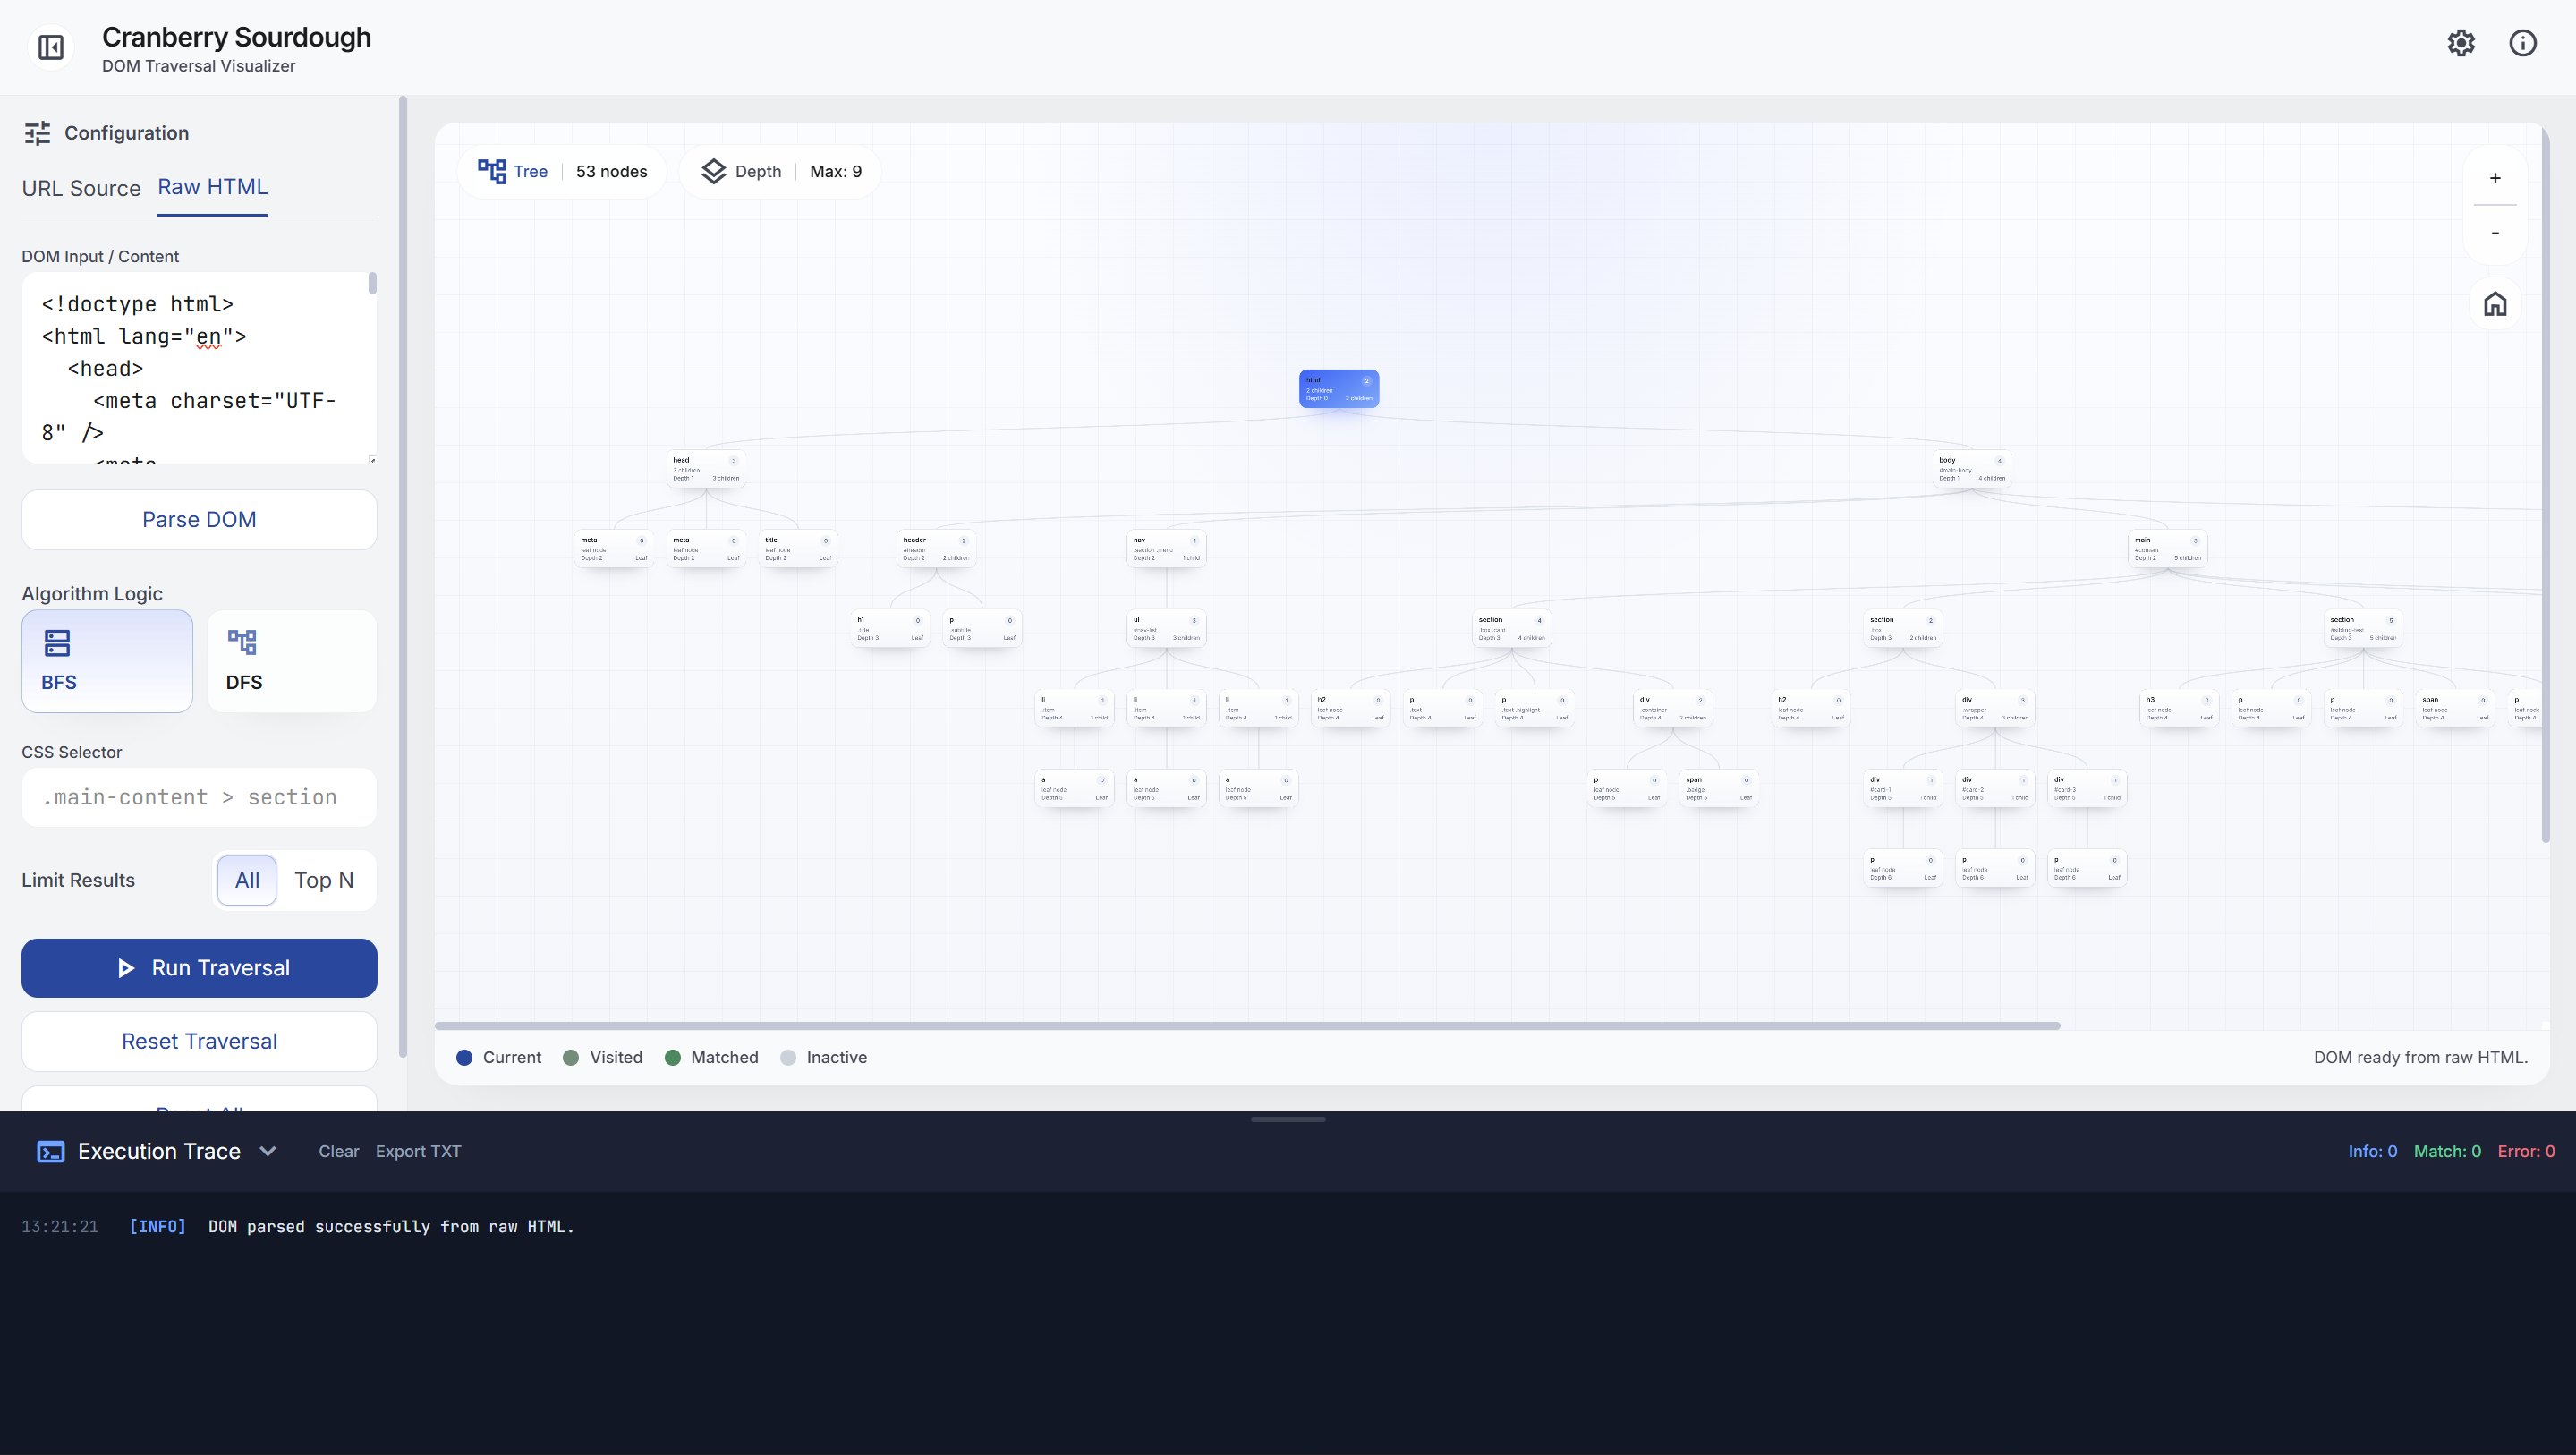
\includegraphics[width=10.5cm]{testcases/01.png}} \\ \hline
\textbf{Expected} & \textbf{Actual} \\ \hline
DOM HTML berhasil diparsing dan struktur tree ditampilkan.
&
Tree DOM muncul serta max depth terhitung. \\ \hline
\end{tabular}
\caption{Pengujian Input DOM HTML}
\end{table}

\subsection{Tag Selector}

\begin{table}[H]
\centering
\renewcommand{\arraystretch}{1.4}
\begin{tabular}{|m{5.4cm}|m{5.4cm}|}
\hline
\multicolumn{2}{|c|}{\textbf{Snippet}} \\ \hline
\multicolumn{2}{|c|}{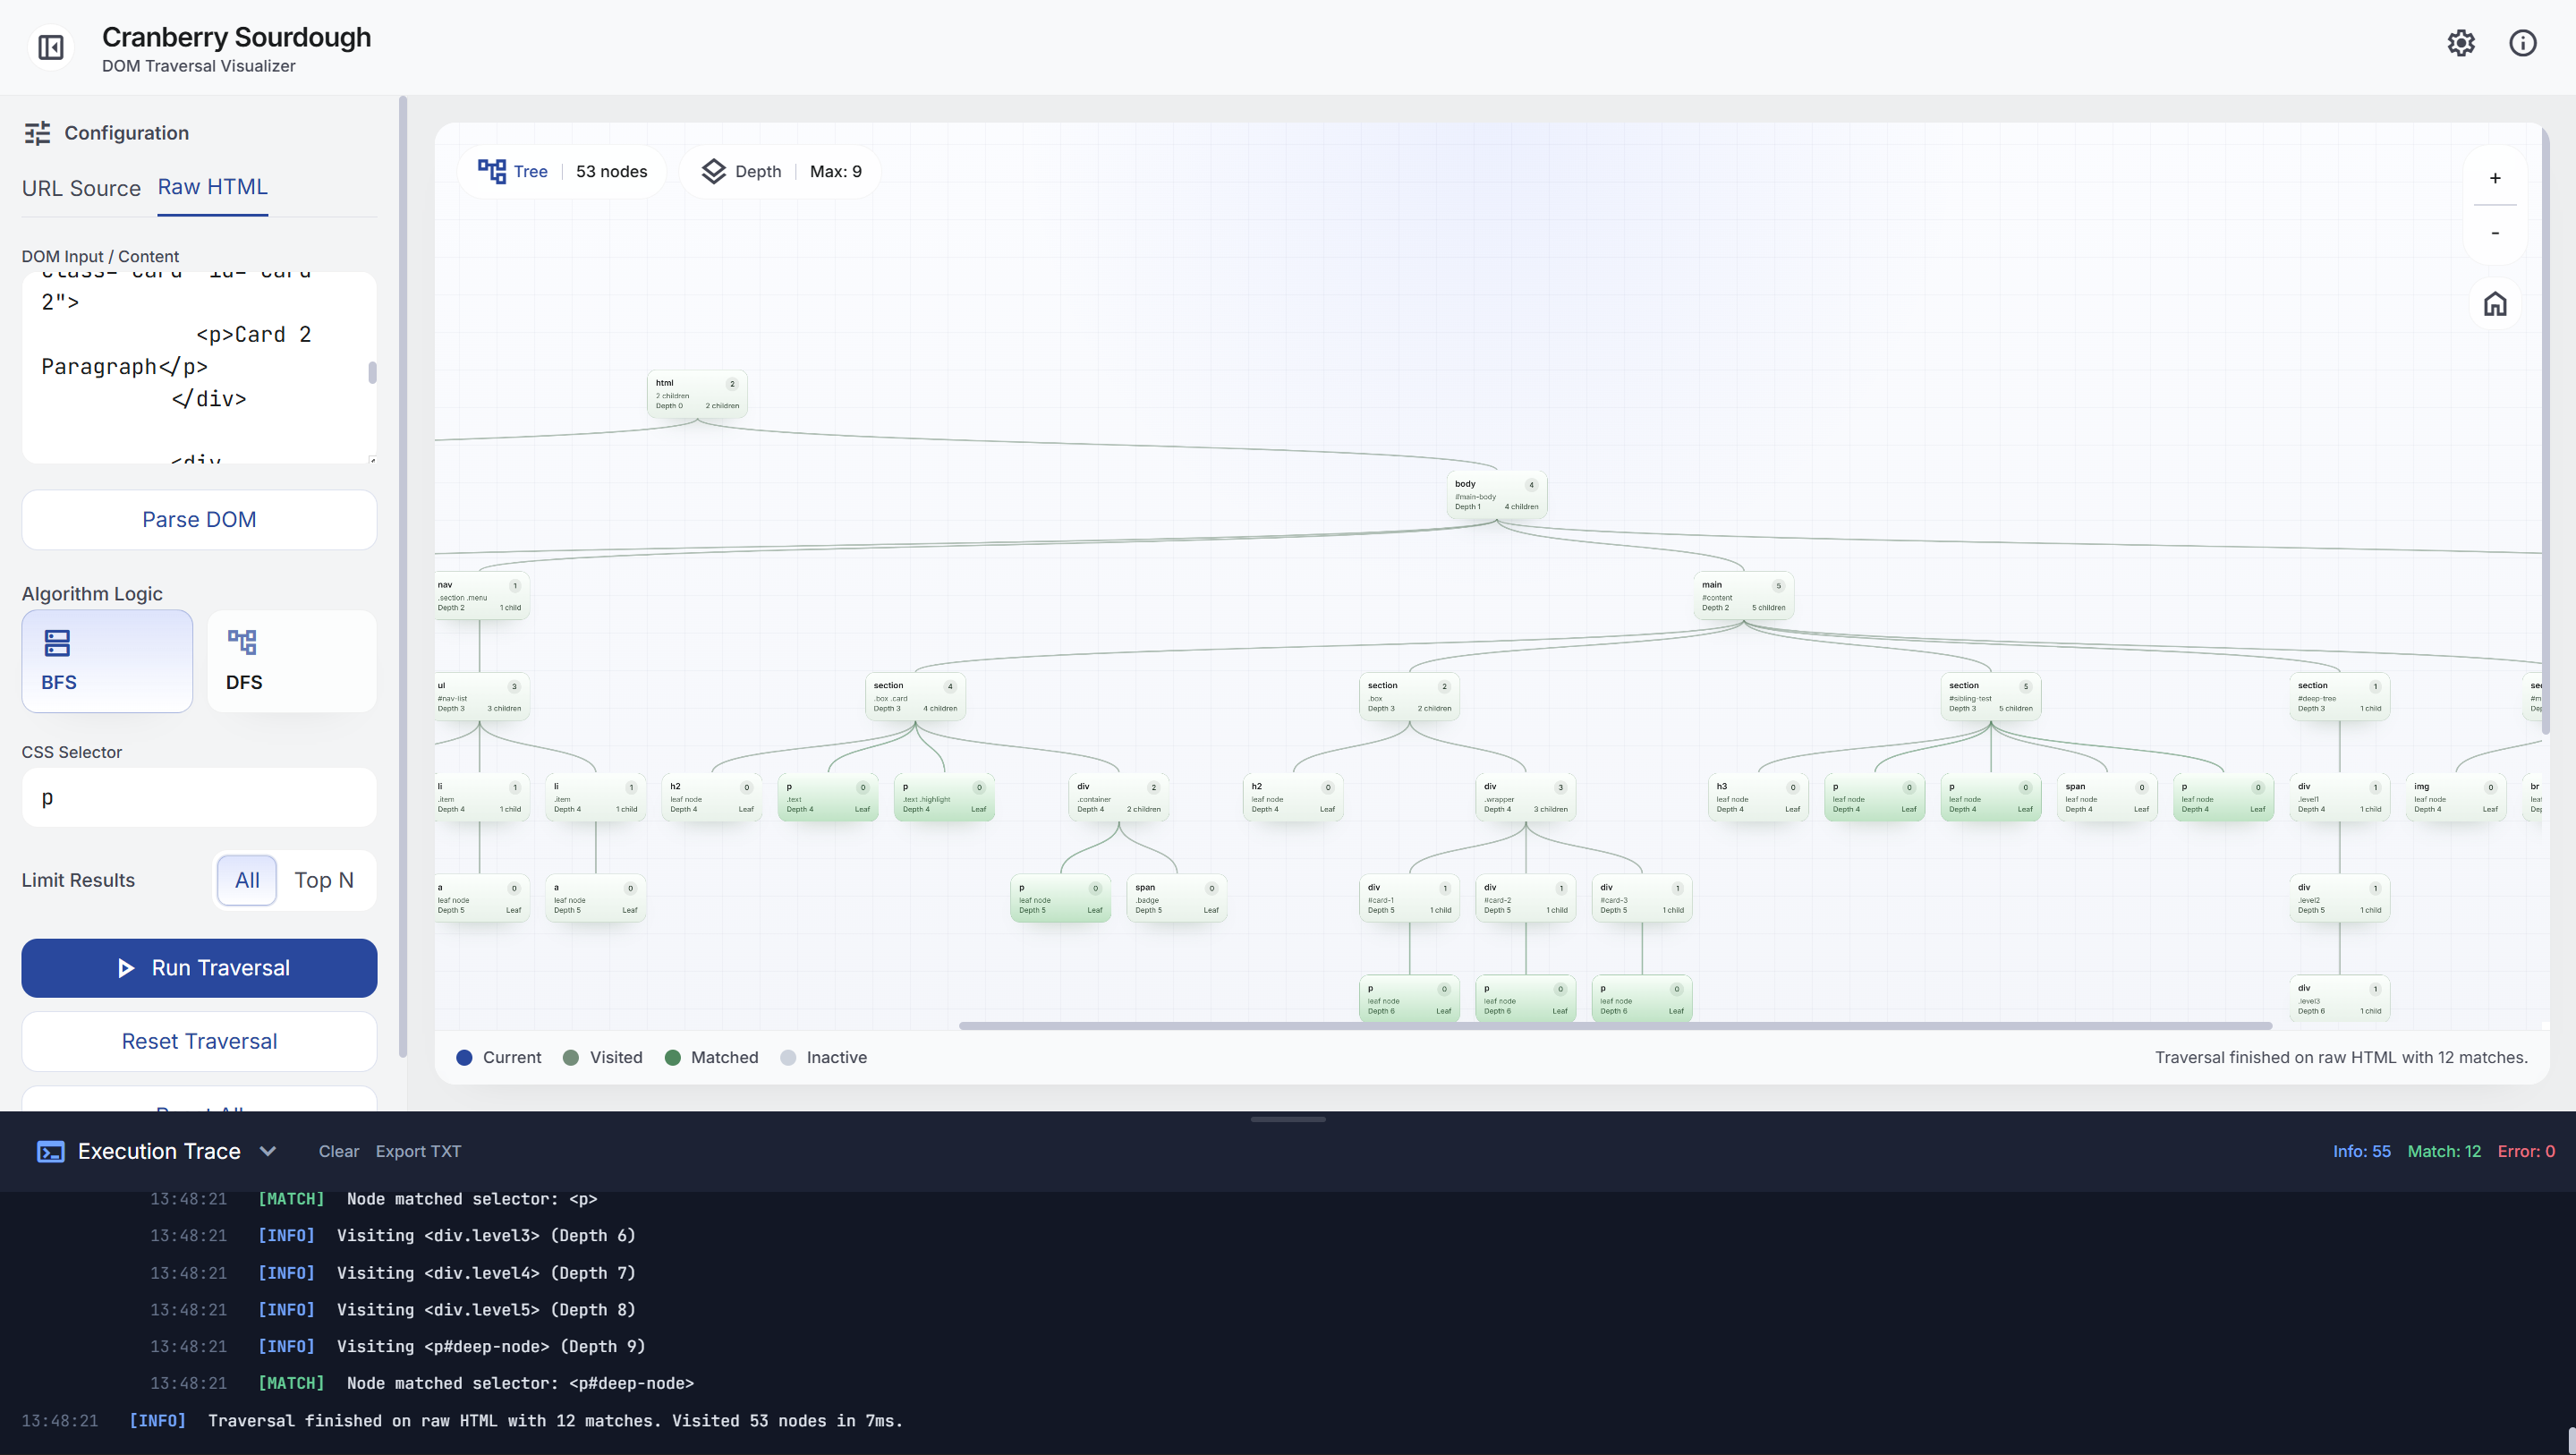
\includegraphics[width=10.5cm]{testcases/02.png}} \\ \hline
\textbf{Expected} & \textbf{Actual} \\ \hline
Selector \texttt{p} menampilkan seluruh elemen paragraf.
&
Seluruh elemen tag p terdeteksi. \\ \hline
\end{tabular}
\caption{Pengujian Tag Selector}
\end{table}

\subsection{Class Selector}

\begin{table}[H]
\centering
\renewcommand{\arraystretch}{1.4} 
\begin{tabular}{|m{5.4cm}|m{5.4cm}|}
\hline
\multicolumn{2}{|c|}{\textbf{Snippet}} \\ \hline
\multicolumn{2}{|c|}{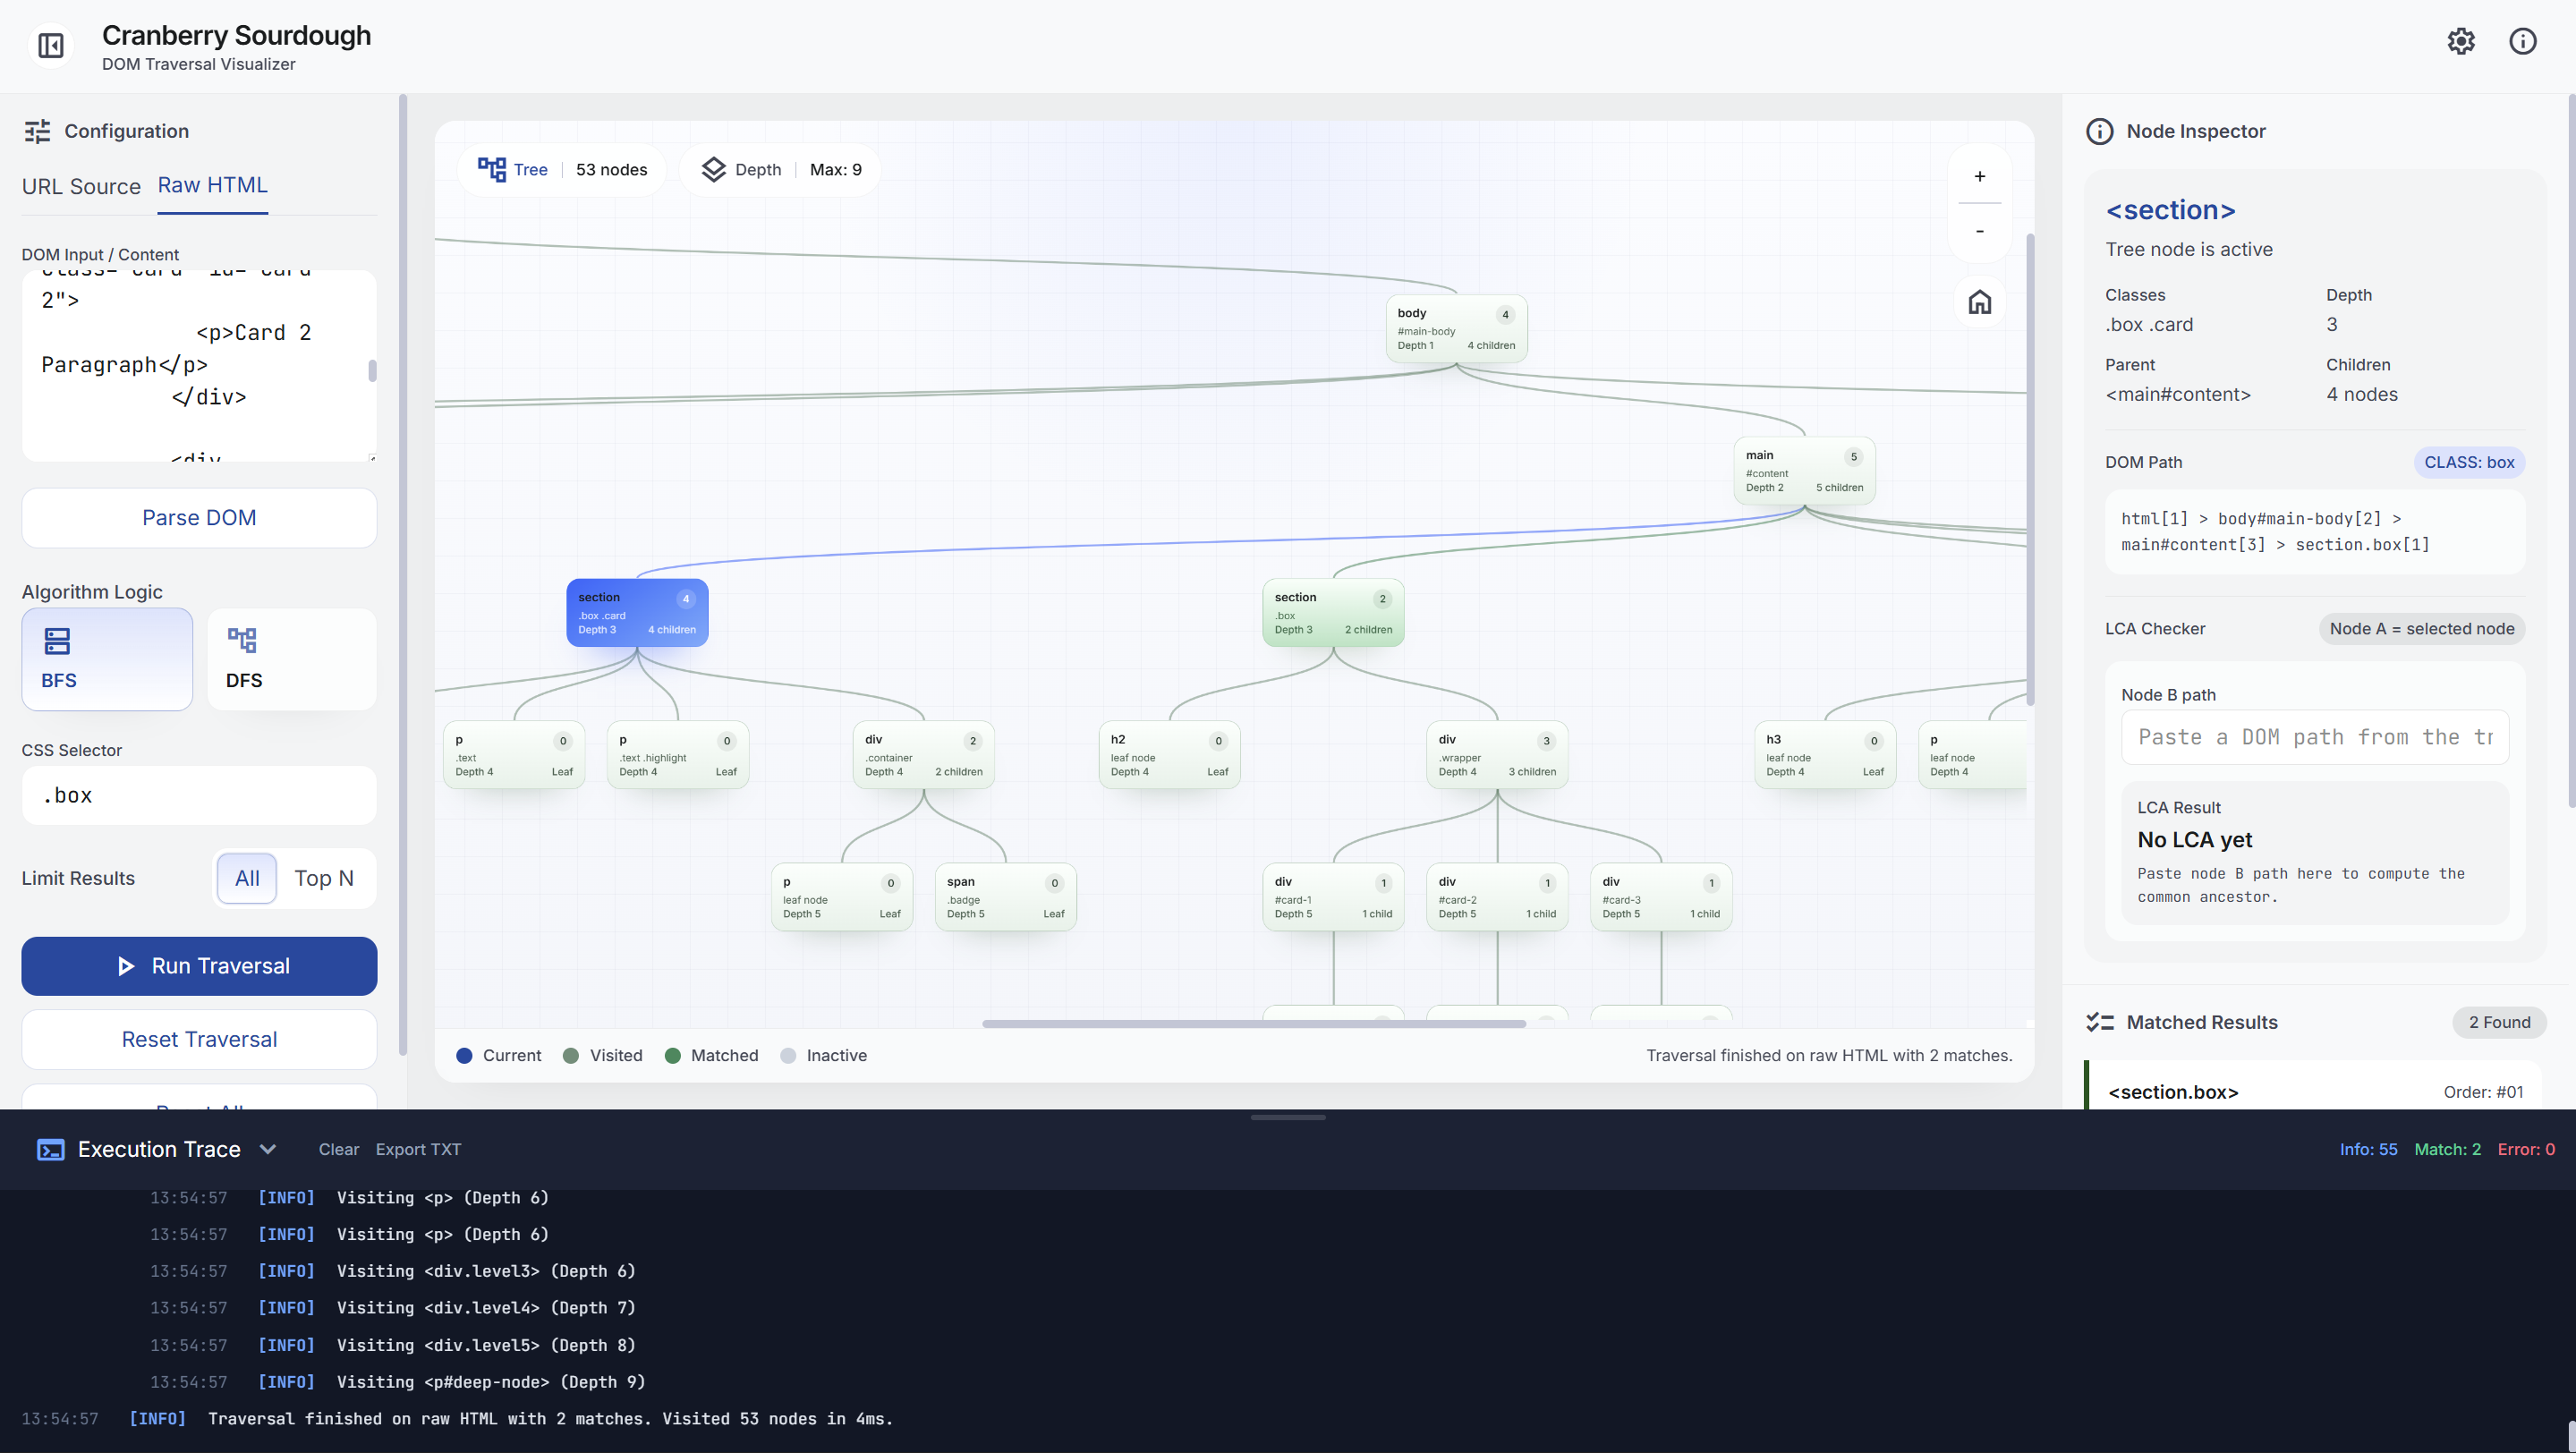
\includegraphics[width=10.5cm]{testcases/03.png}} \\ \hline
\textbf{Expected} & \textbf{Actual} \\ \hline
Selector \texttt{.box} menampilkan seluruh elemen dengan class box.
&
Elemen dengan class box terdeteksi. \\ \hline
\end{tabular}
\caption{Pengujian Class Selector}
\end{table}

\subsection{ID Selector}

\begin{table}[H]
\centering
\renewcommand{\arraystretch}{1.4}
\begin{tabular}{|m{5.4cm}|m{5.4cm}|}
\hline
\multicolumn{2}{|c|}{\textbf{Snippet}} \\ \hline
\multicolumn{2}{|c|}{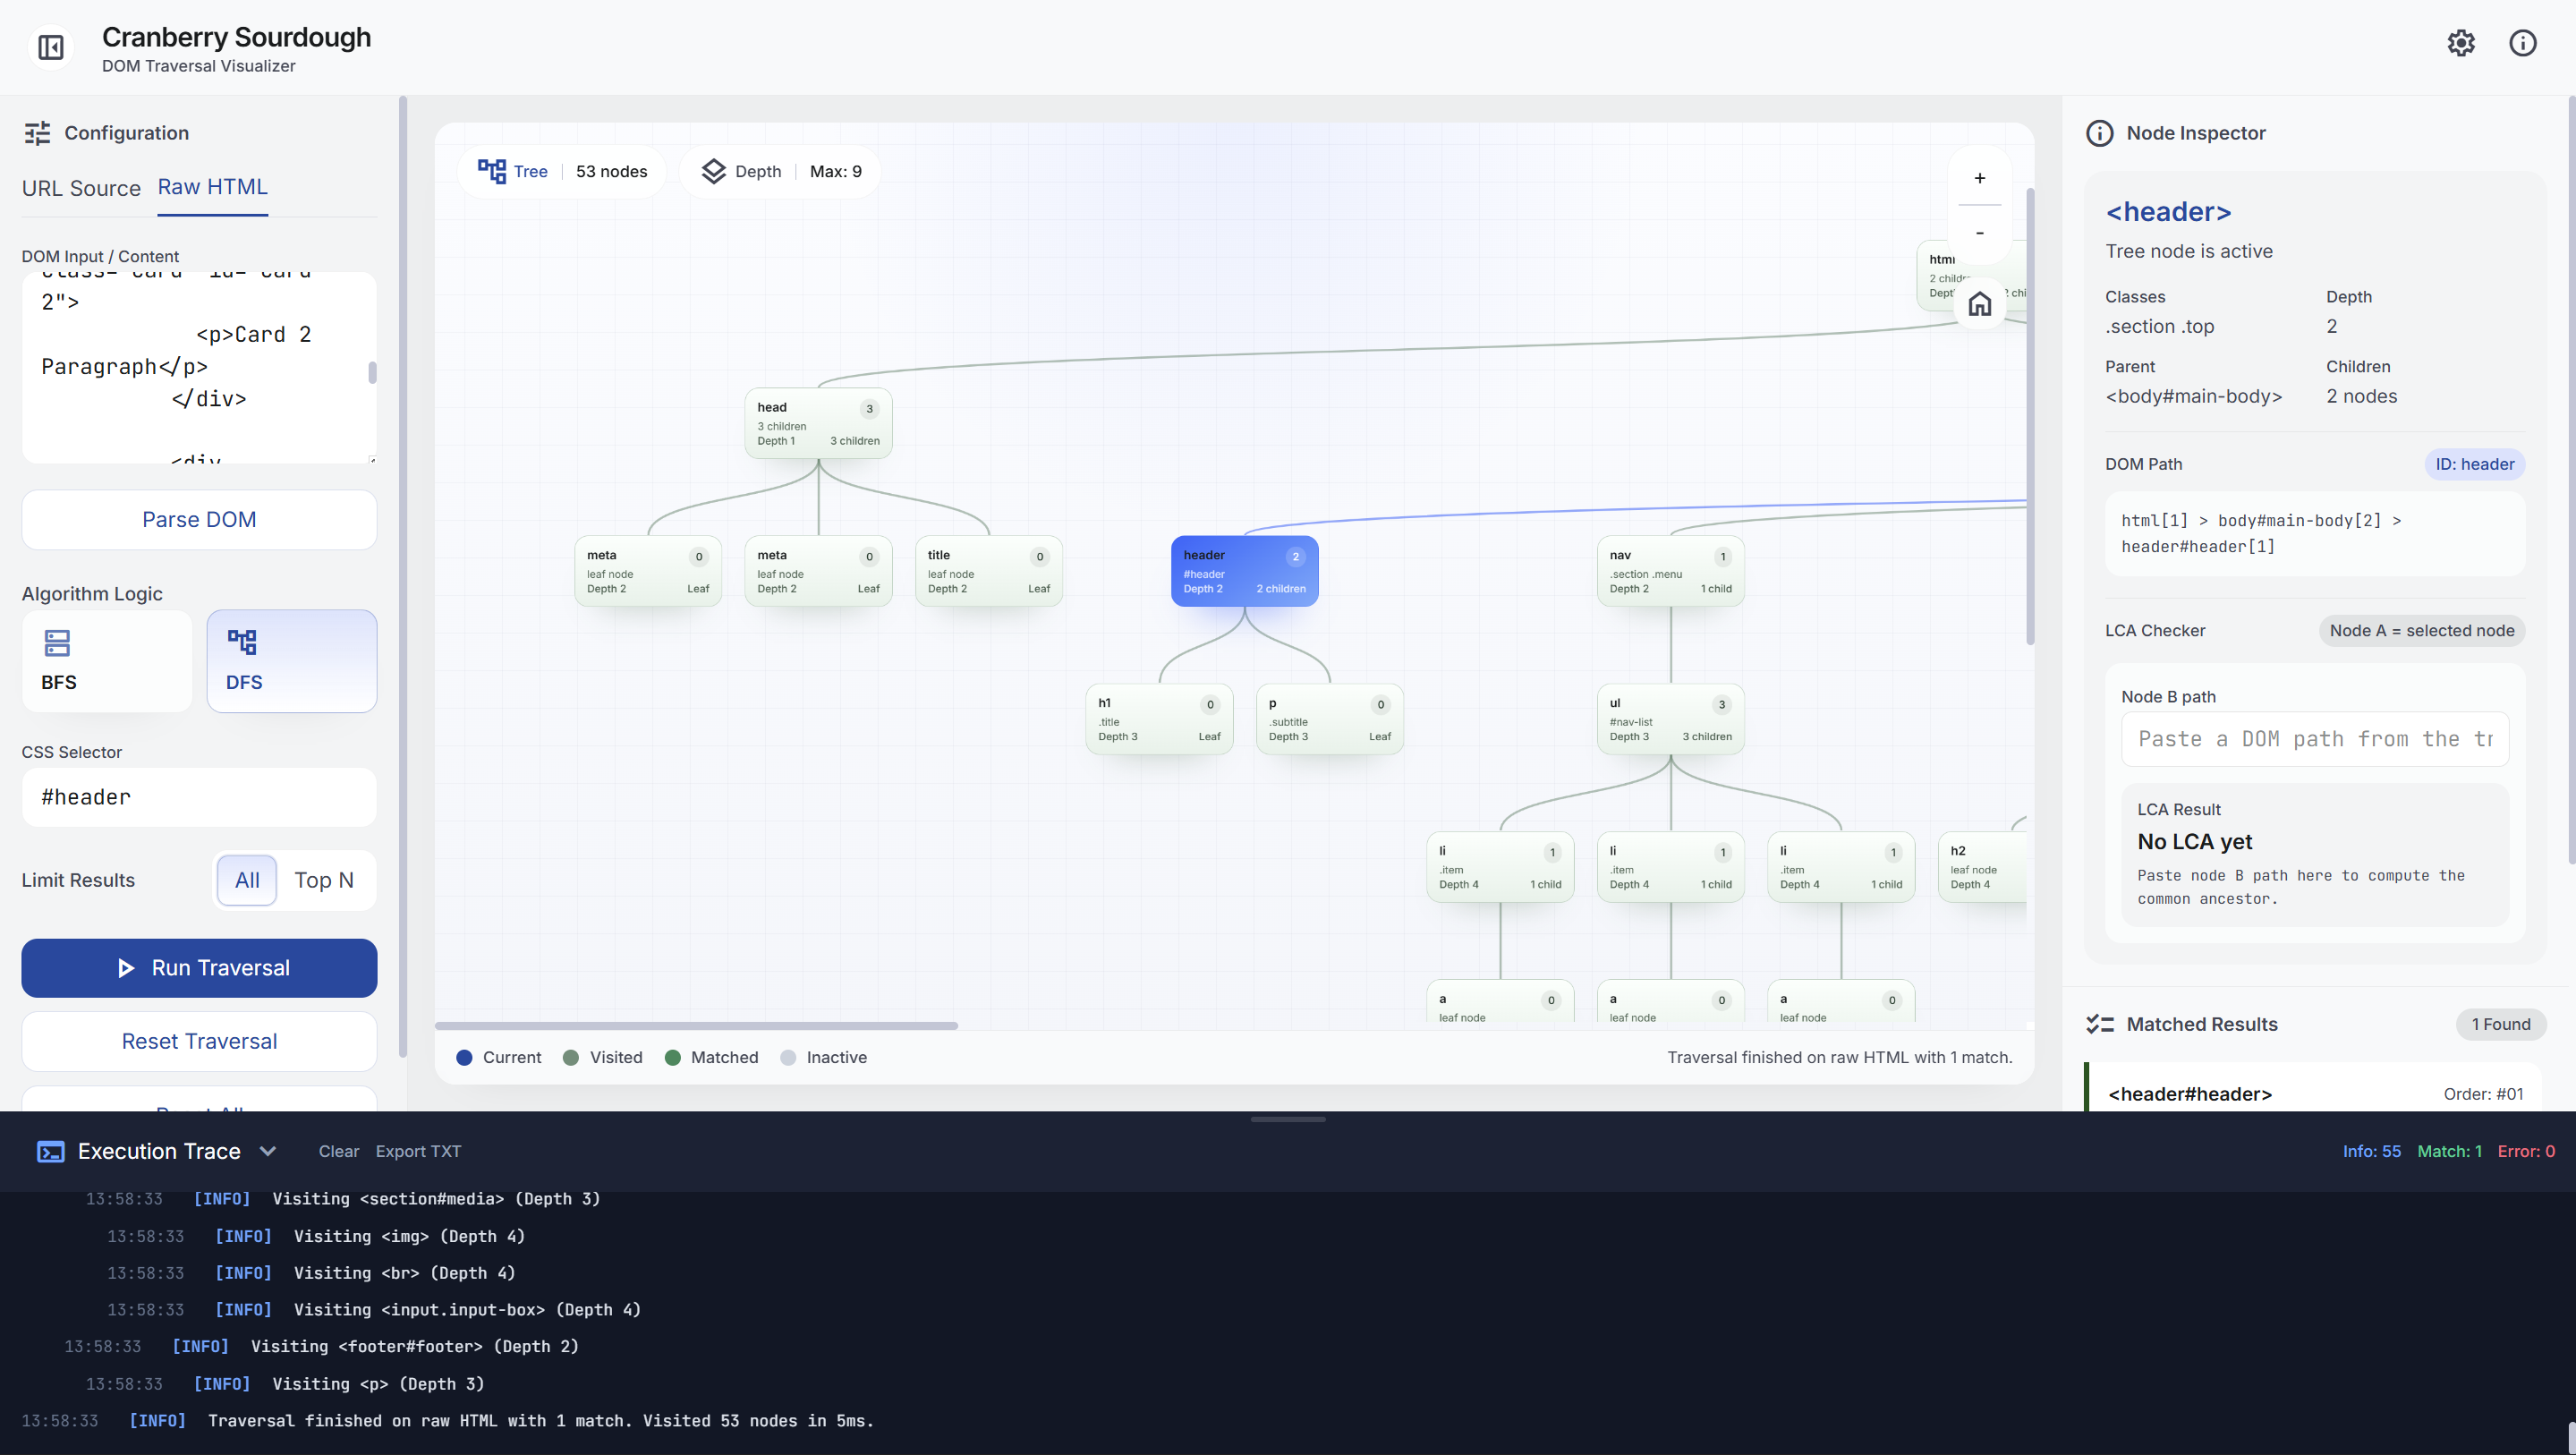
\includegraphics[width=10.5cm]{testcases/04.png}} \\ \hline
\textbf{Expected} & \textbf{Actual} \\ \hline
Selector \texttt{\#header} menampilkan satu elemen dengan id header.
&
Elemen dengan id header terdeteksi. \\ \hline
\end{tabular}
\caption{Pengujian ID Selector}
\end{table}

\subsection{Universal Selector}

\begin{table}[H]
\centering
\renewcommand{\arraystretch}{1.4}
\begin{tabular}{|m{5.4cm}|m{5.4cm}|}
\hline
\multicolumn{2}{|c|}{\textbf{Snippet}} \\ \hline
\multicolumn{2}{|c|}{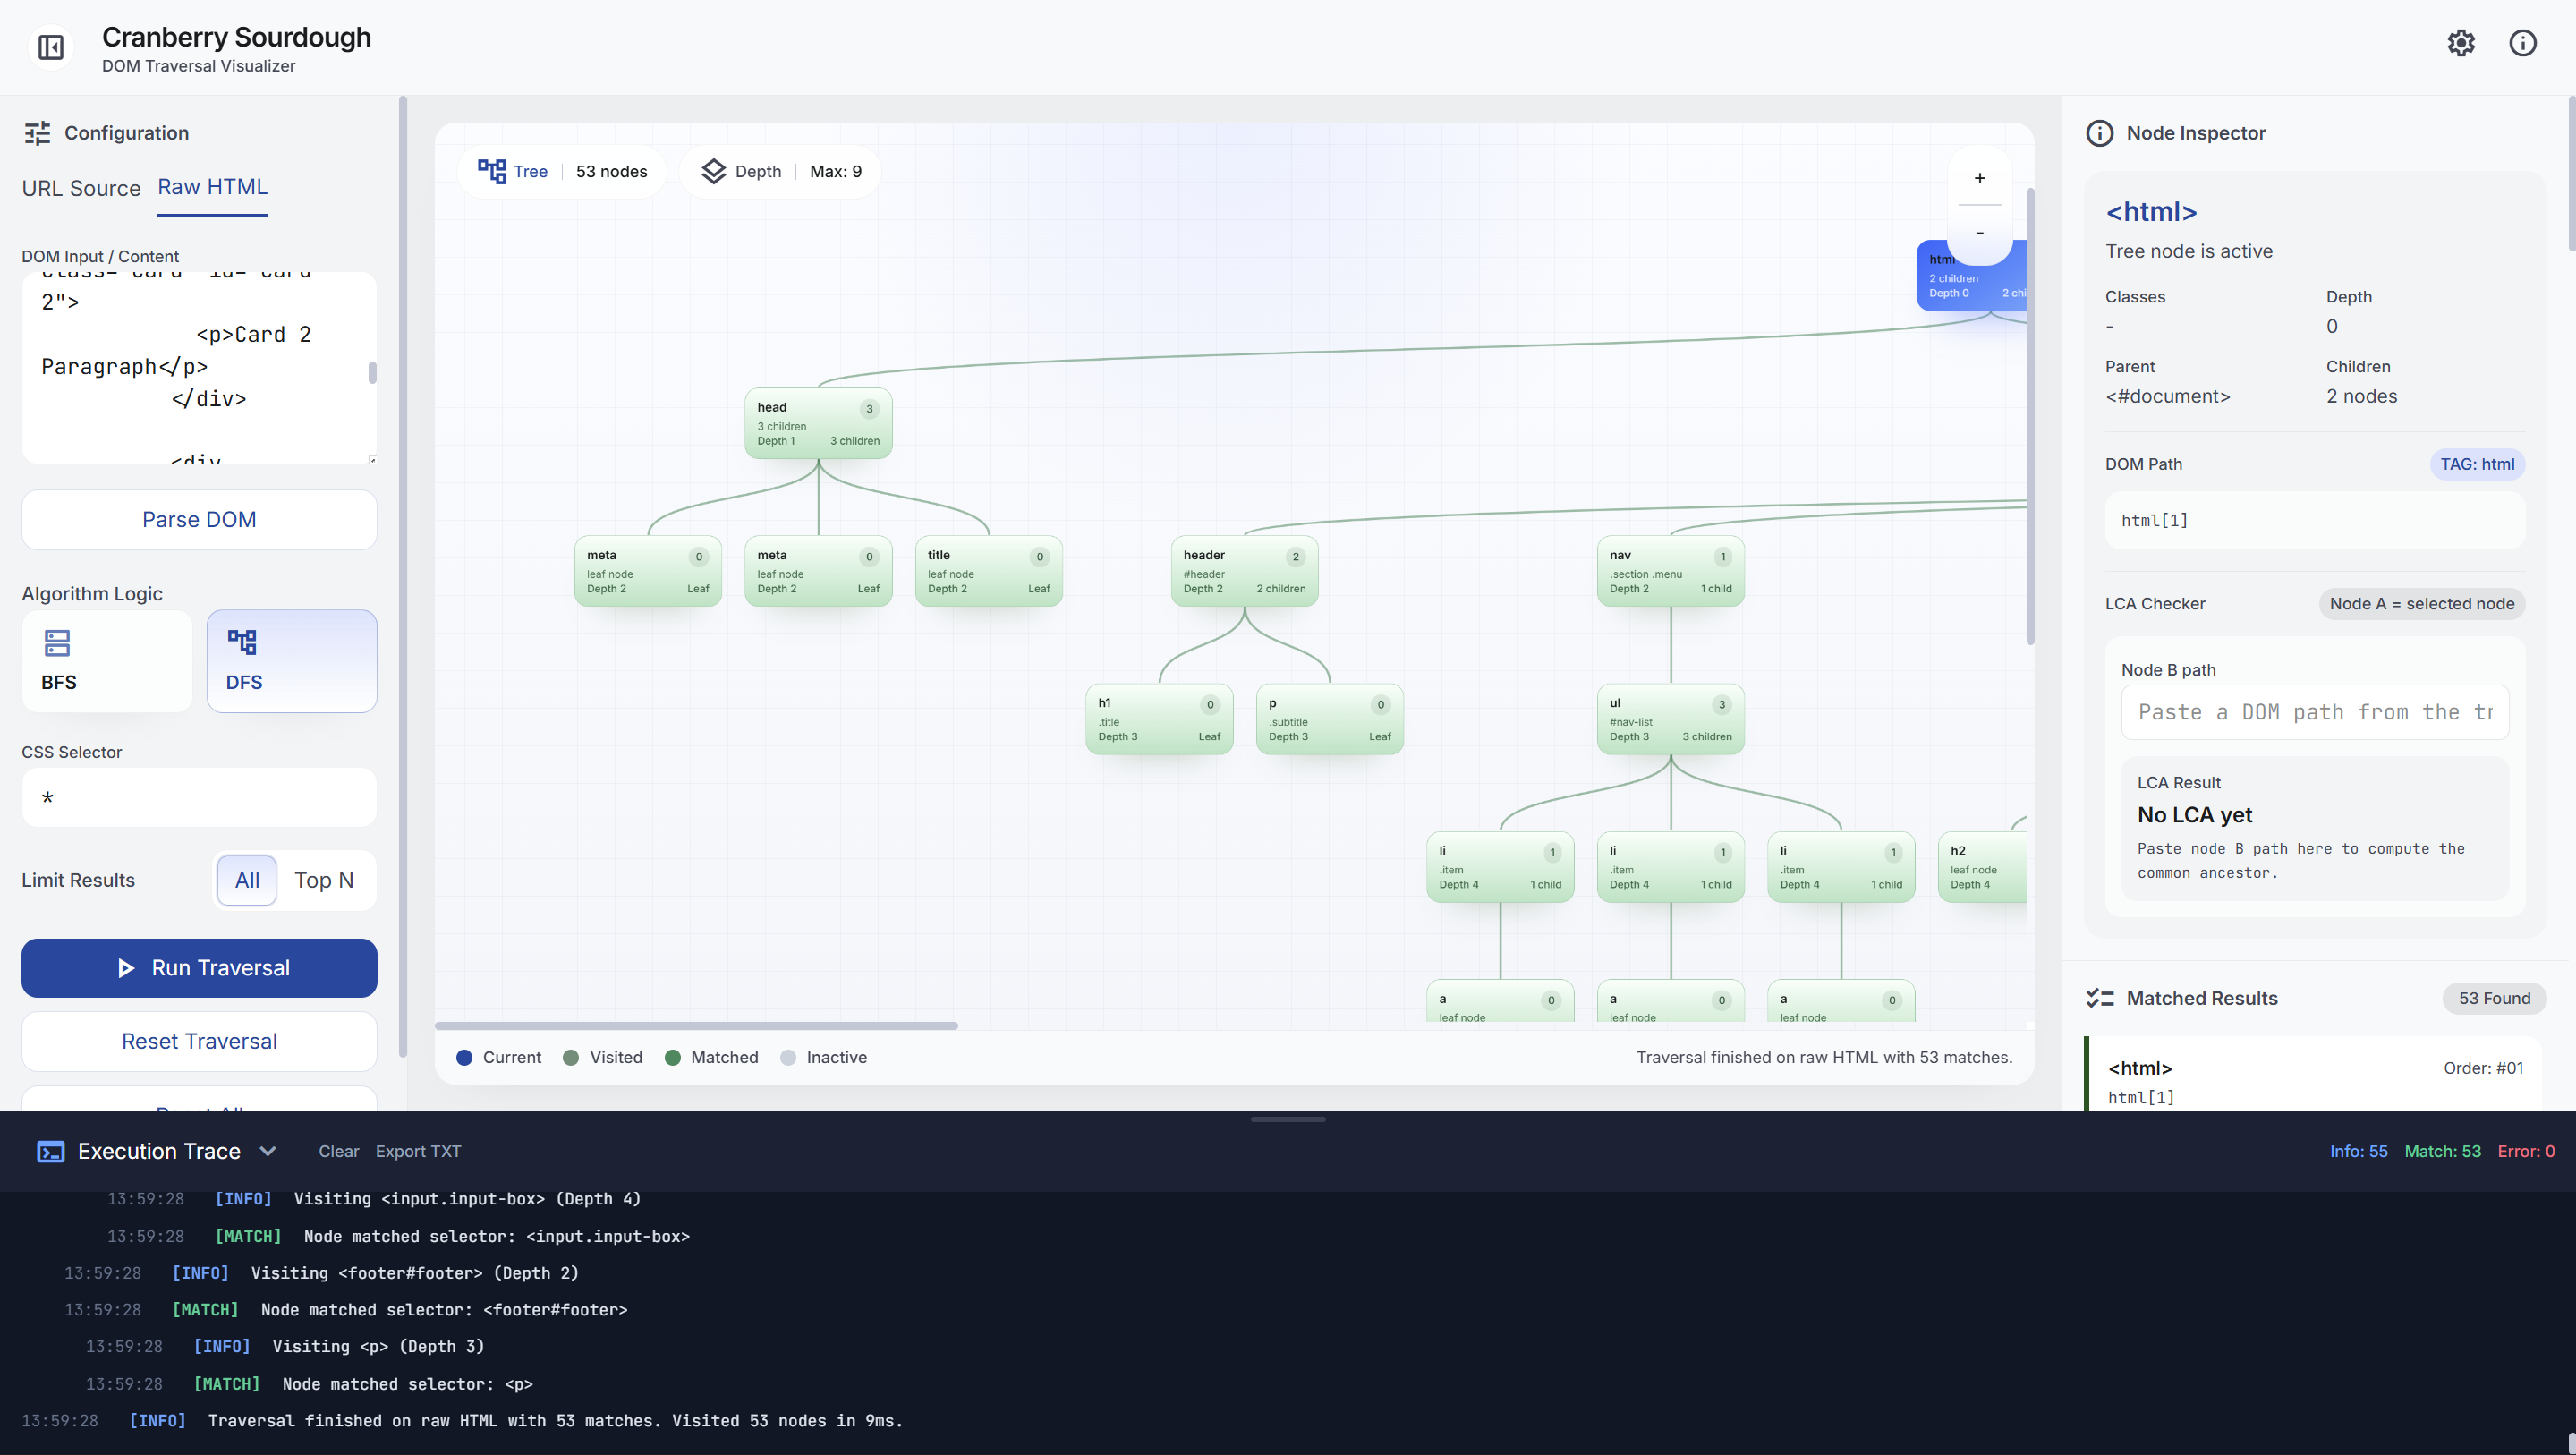
\includegraphics[width=10.5cm]{testcases/05.png}} \\ \hline
\textbf{Expected} & \textbf{Actual} \\ \hline
Selector \texttt{*} menampilkan seluruh node DOM.
&
Seluruh elemen terdeteksi. \\ \hline
\end{tabular}
\caption{Pengujian Universal Selector}
\end{table}

\subsection{Child Combinator}

\begin{table}[H]
\centering
\renewcommand{\arraystretch}{1.4}
\begin{tabular}{|m{5.4cm}|m{5.4cm}|}
\hline
\multicolumn{2}{|c|}{\textbf{Snippet}} \\ \hline
\multicolumn{2}{|c|}{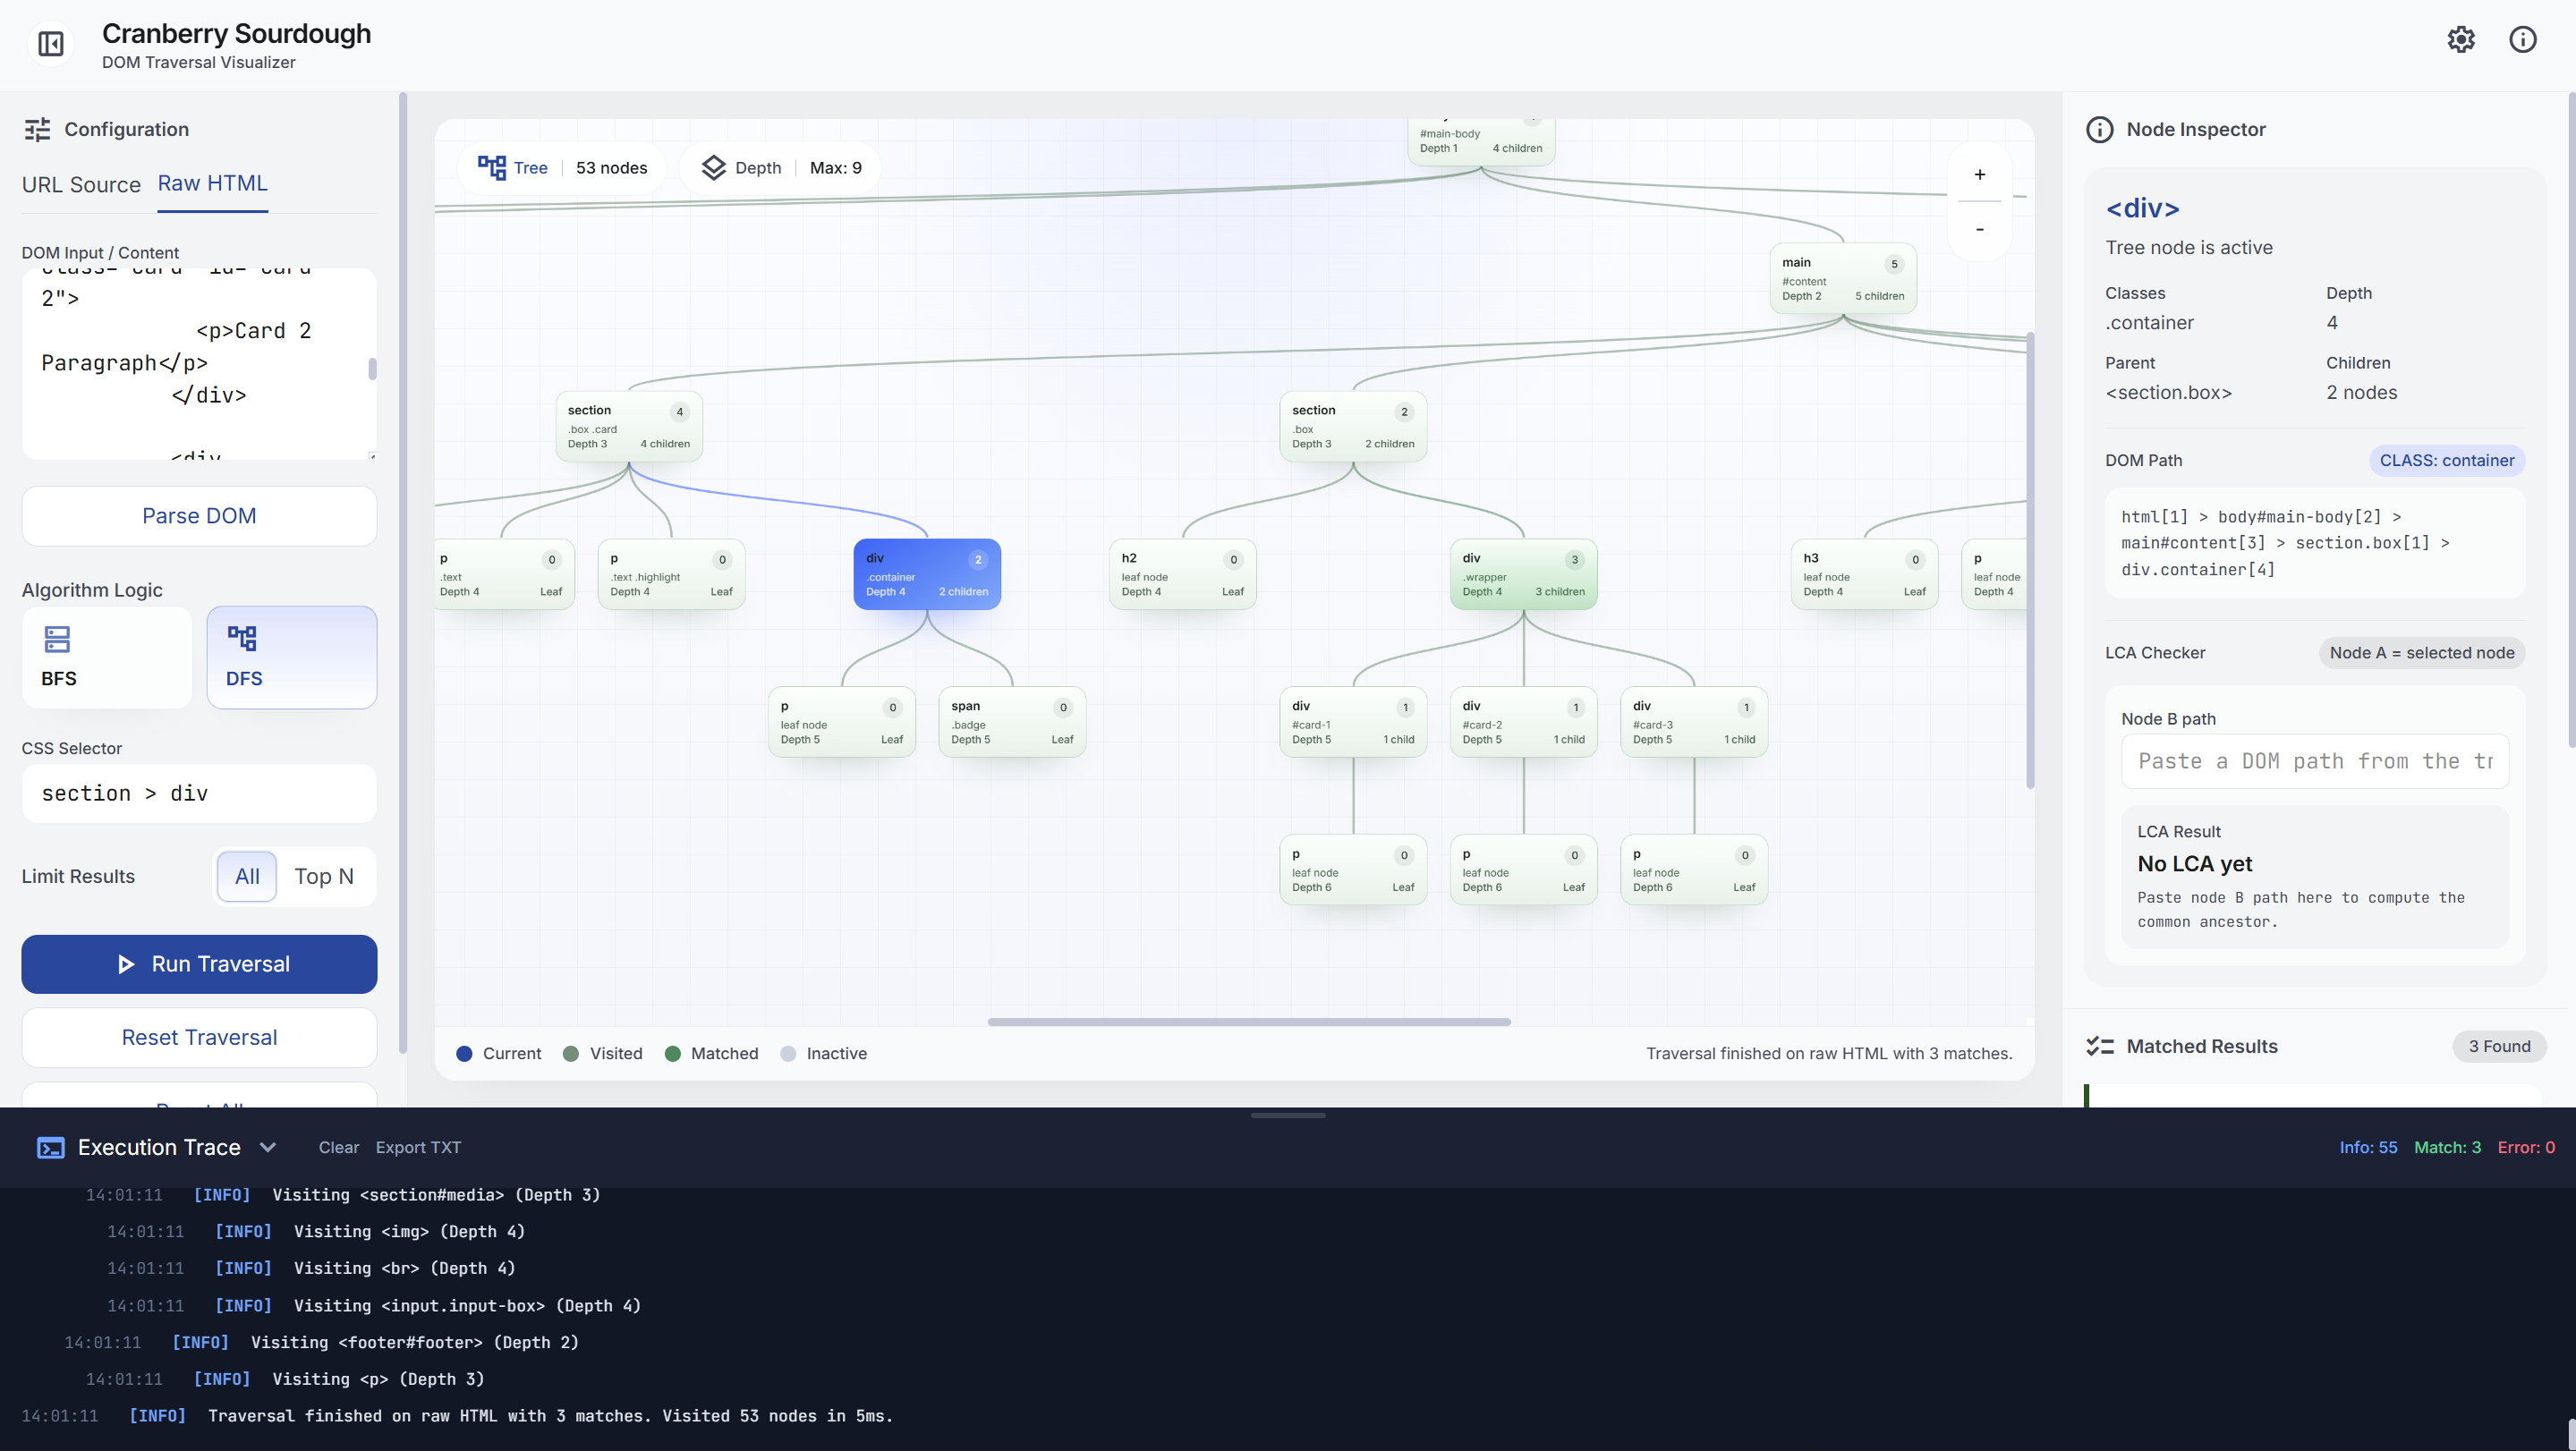
\includegraphics[width=10.5cm]{testcases/06.png}} \\ \hline
\textbf{Expected} & \textbf{Actual} \\ \hline
Selector \texttt{div > p} menampilkan child langsung.
&
tag p yang merupakan child langsung dari div terdeteksi. \\ \hline
\end{tabular}
\caption{Pengujian Child Combinator}
\end{table}

\subsection{Descendant Combinator}

\begin{table}[H]
\centering
\renewcommand{\arraystretch}{1.4}
\begin{tabular}{|m{5.4cm}|m{5.4cm}|}
\hline
\multicolumn{2}{|c|}{\textbf{Snippet}} \\ \hline
\multicolumn{2}{|c|}{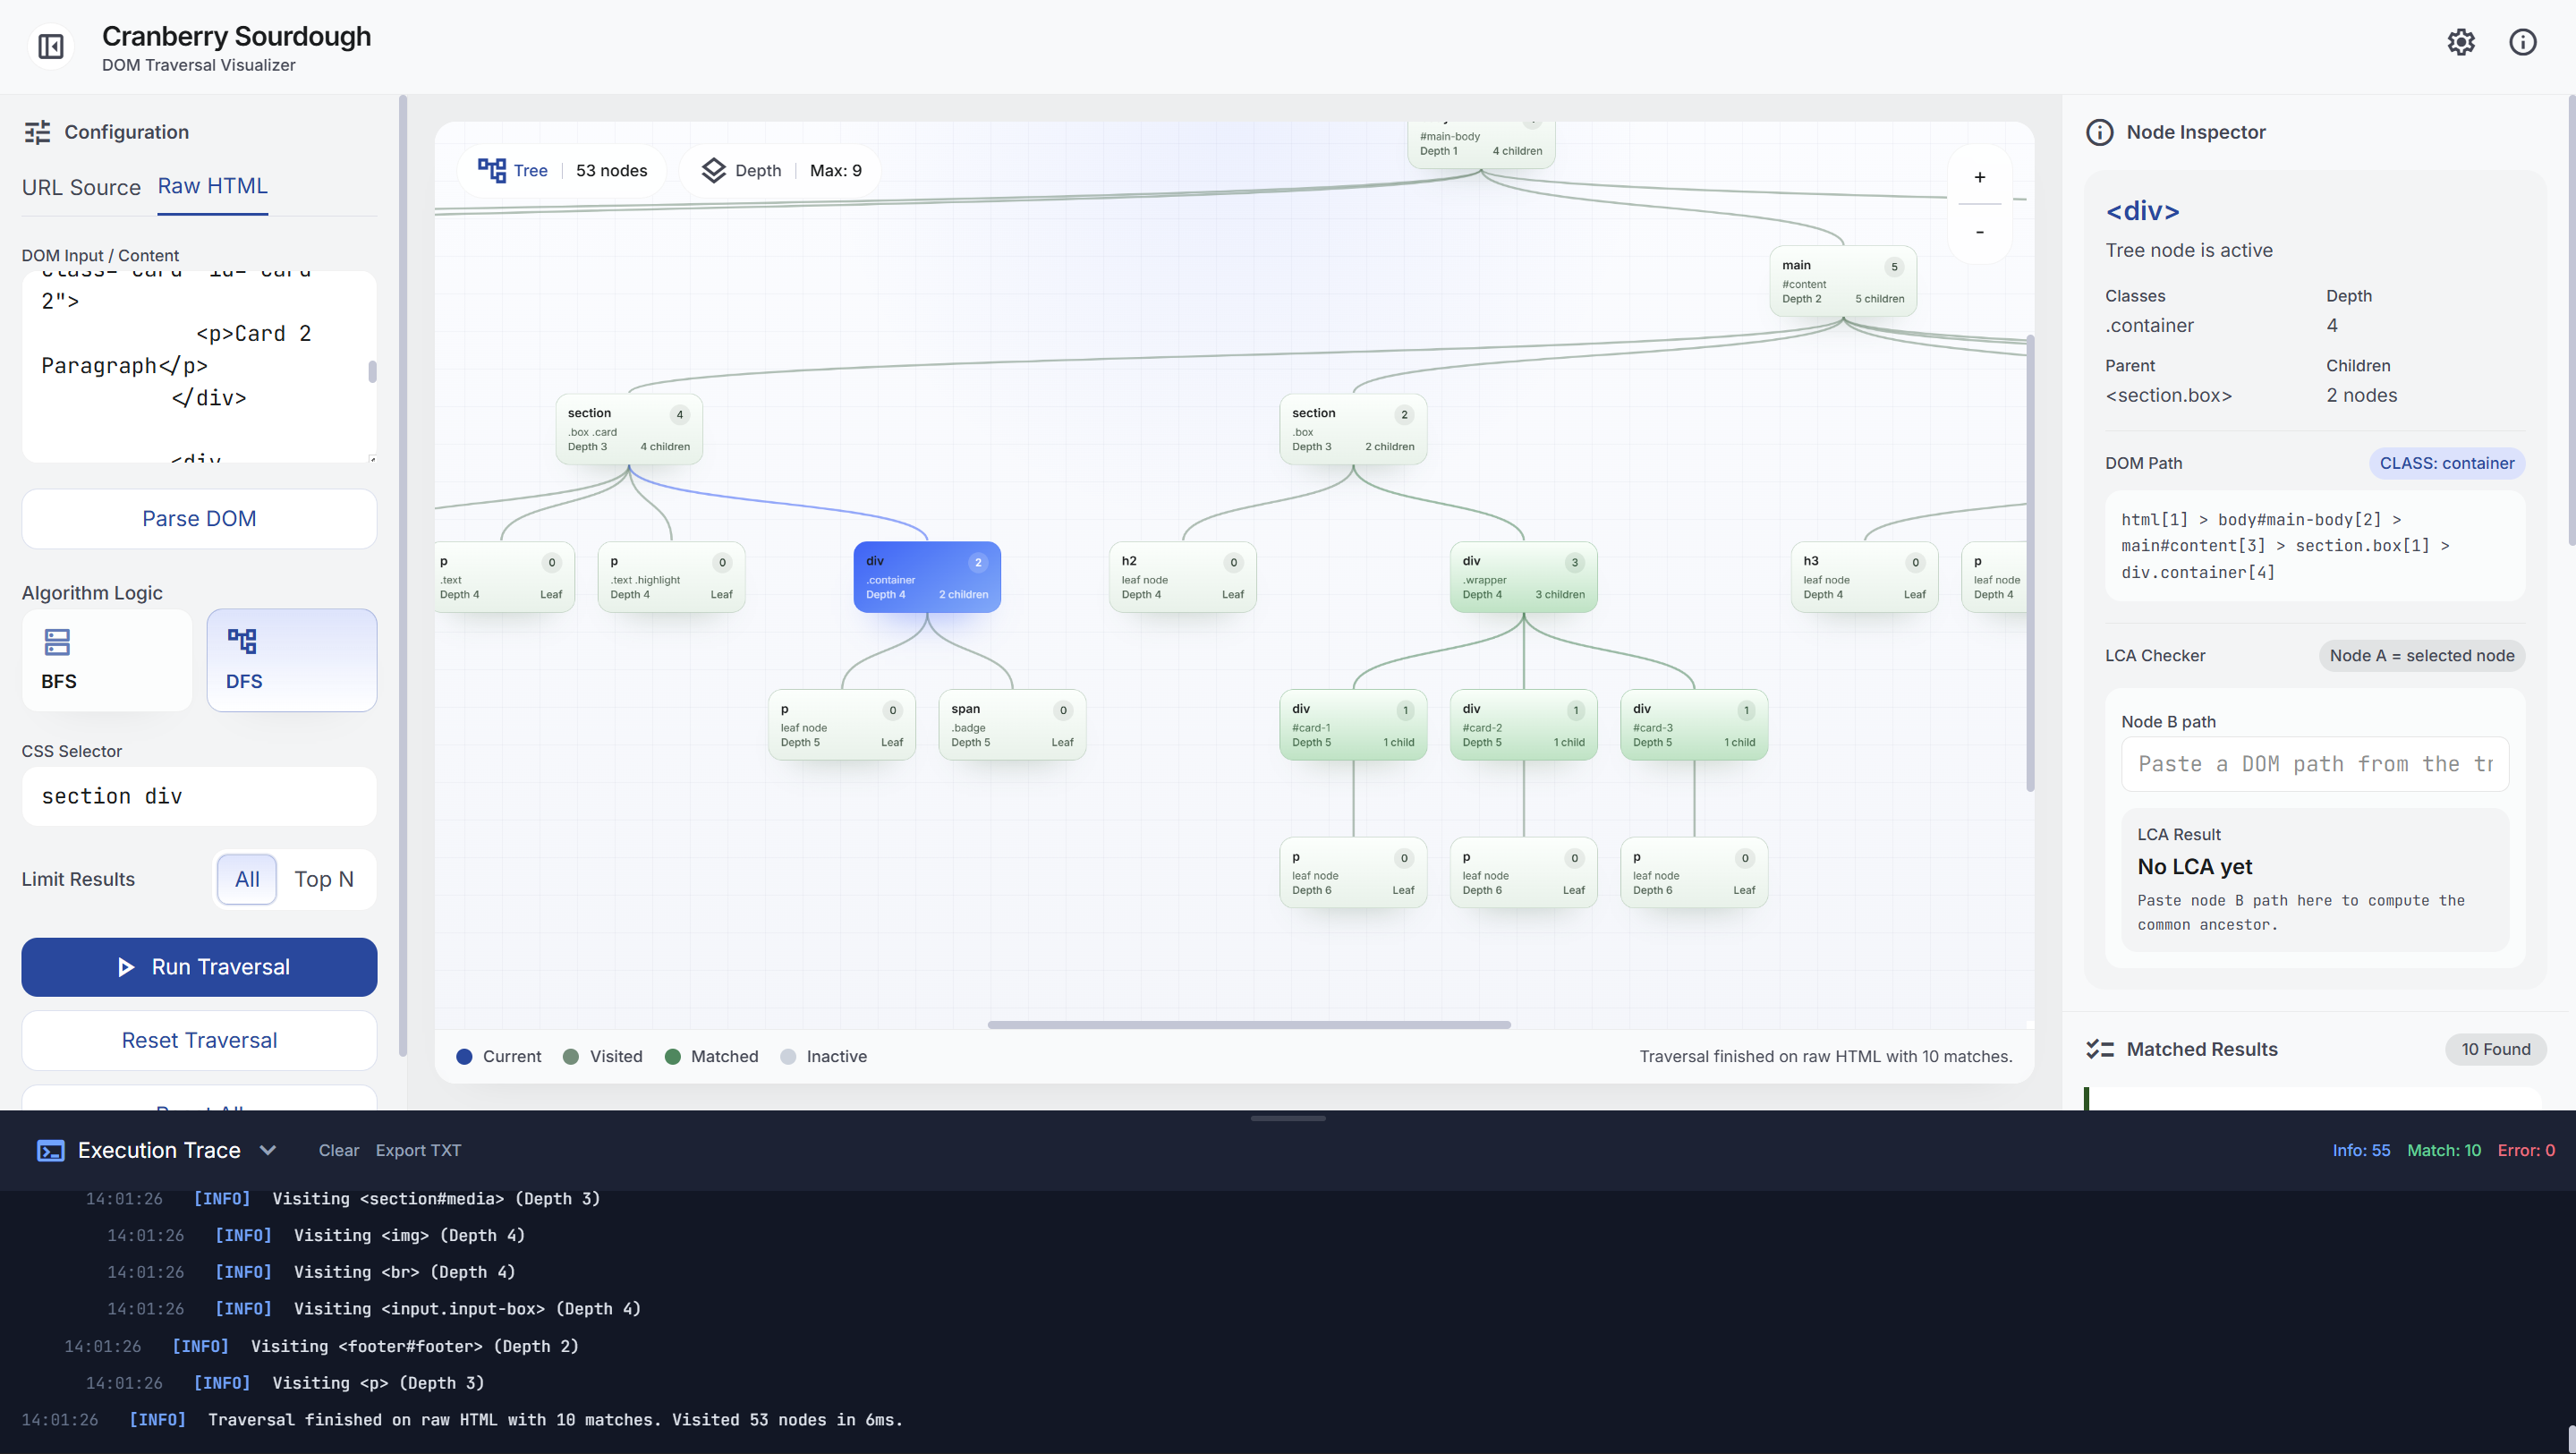
\includegraphics[width=10.5cm]{testcases/07.png}} \\ \hline
\textbf{Expected} & \textbf{Actual} \\ \hline
Selector \texttt{div p} menampilkan seluruh descendant.
&
tag p yang merupakan descendant (tidak harus direct child) dari div terdeteksi. \\ \hline
\end{tabular}
\caption{Pengujian Descendant Combinator}
\end{table}

\subsection{Adjacent Sibling}

\begin{table}[H]
\centering
\renewcommand{\arraystretch}{1.4}
\begin{tabular}{|m{5.4cm}|m{5.4cm}|}
\hline
\multicolumn{2}{|c|}{\textbf{Snippet}} \\ \hline
\multicolumn{2}{|c|}{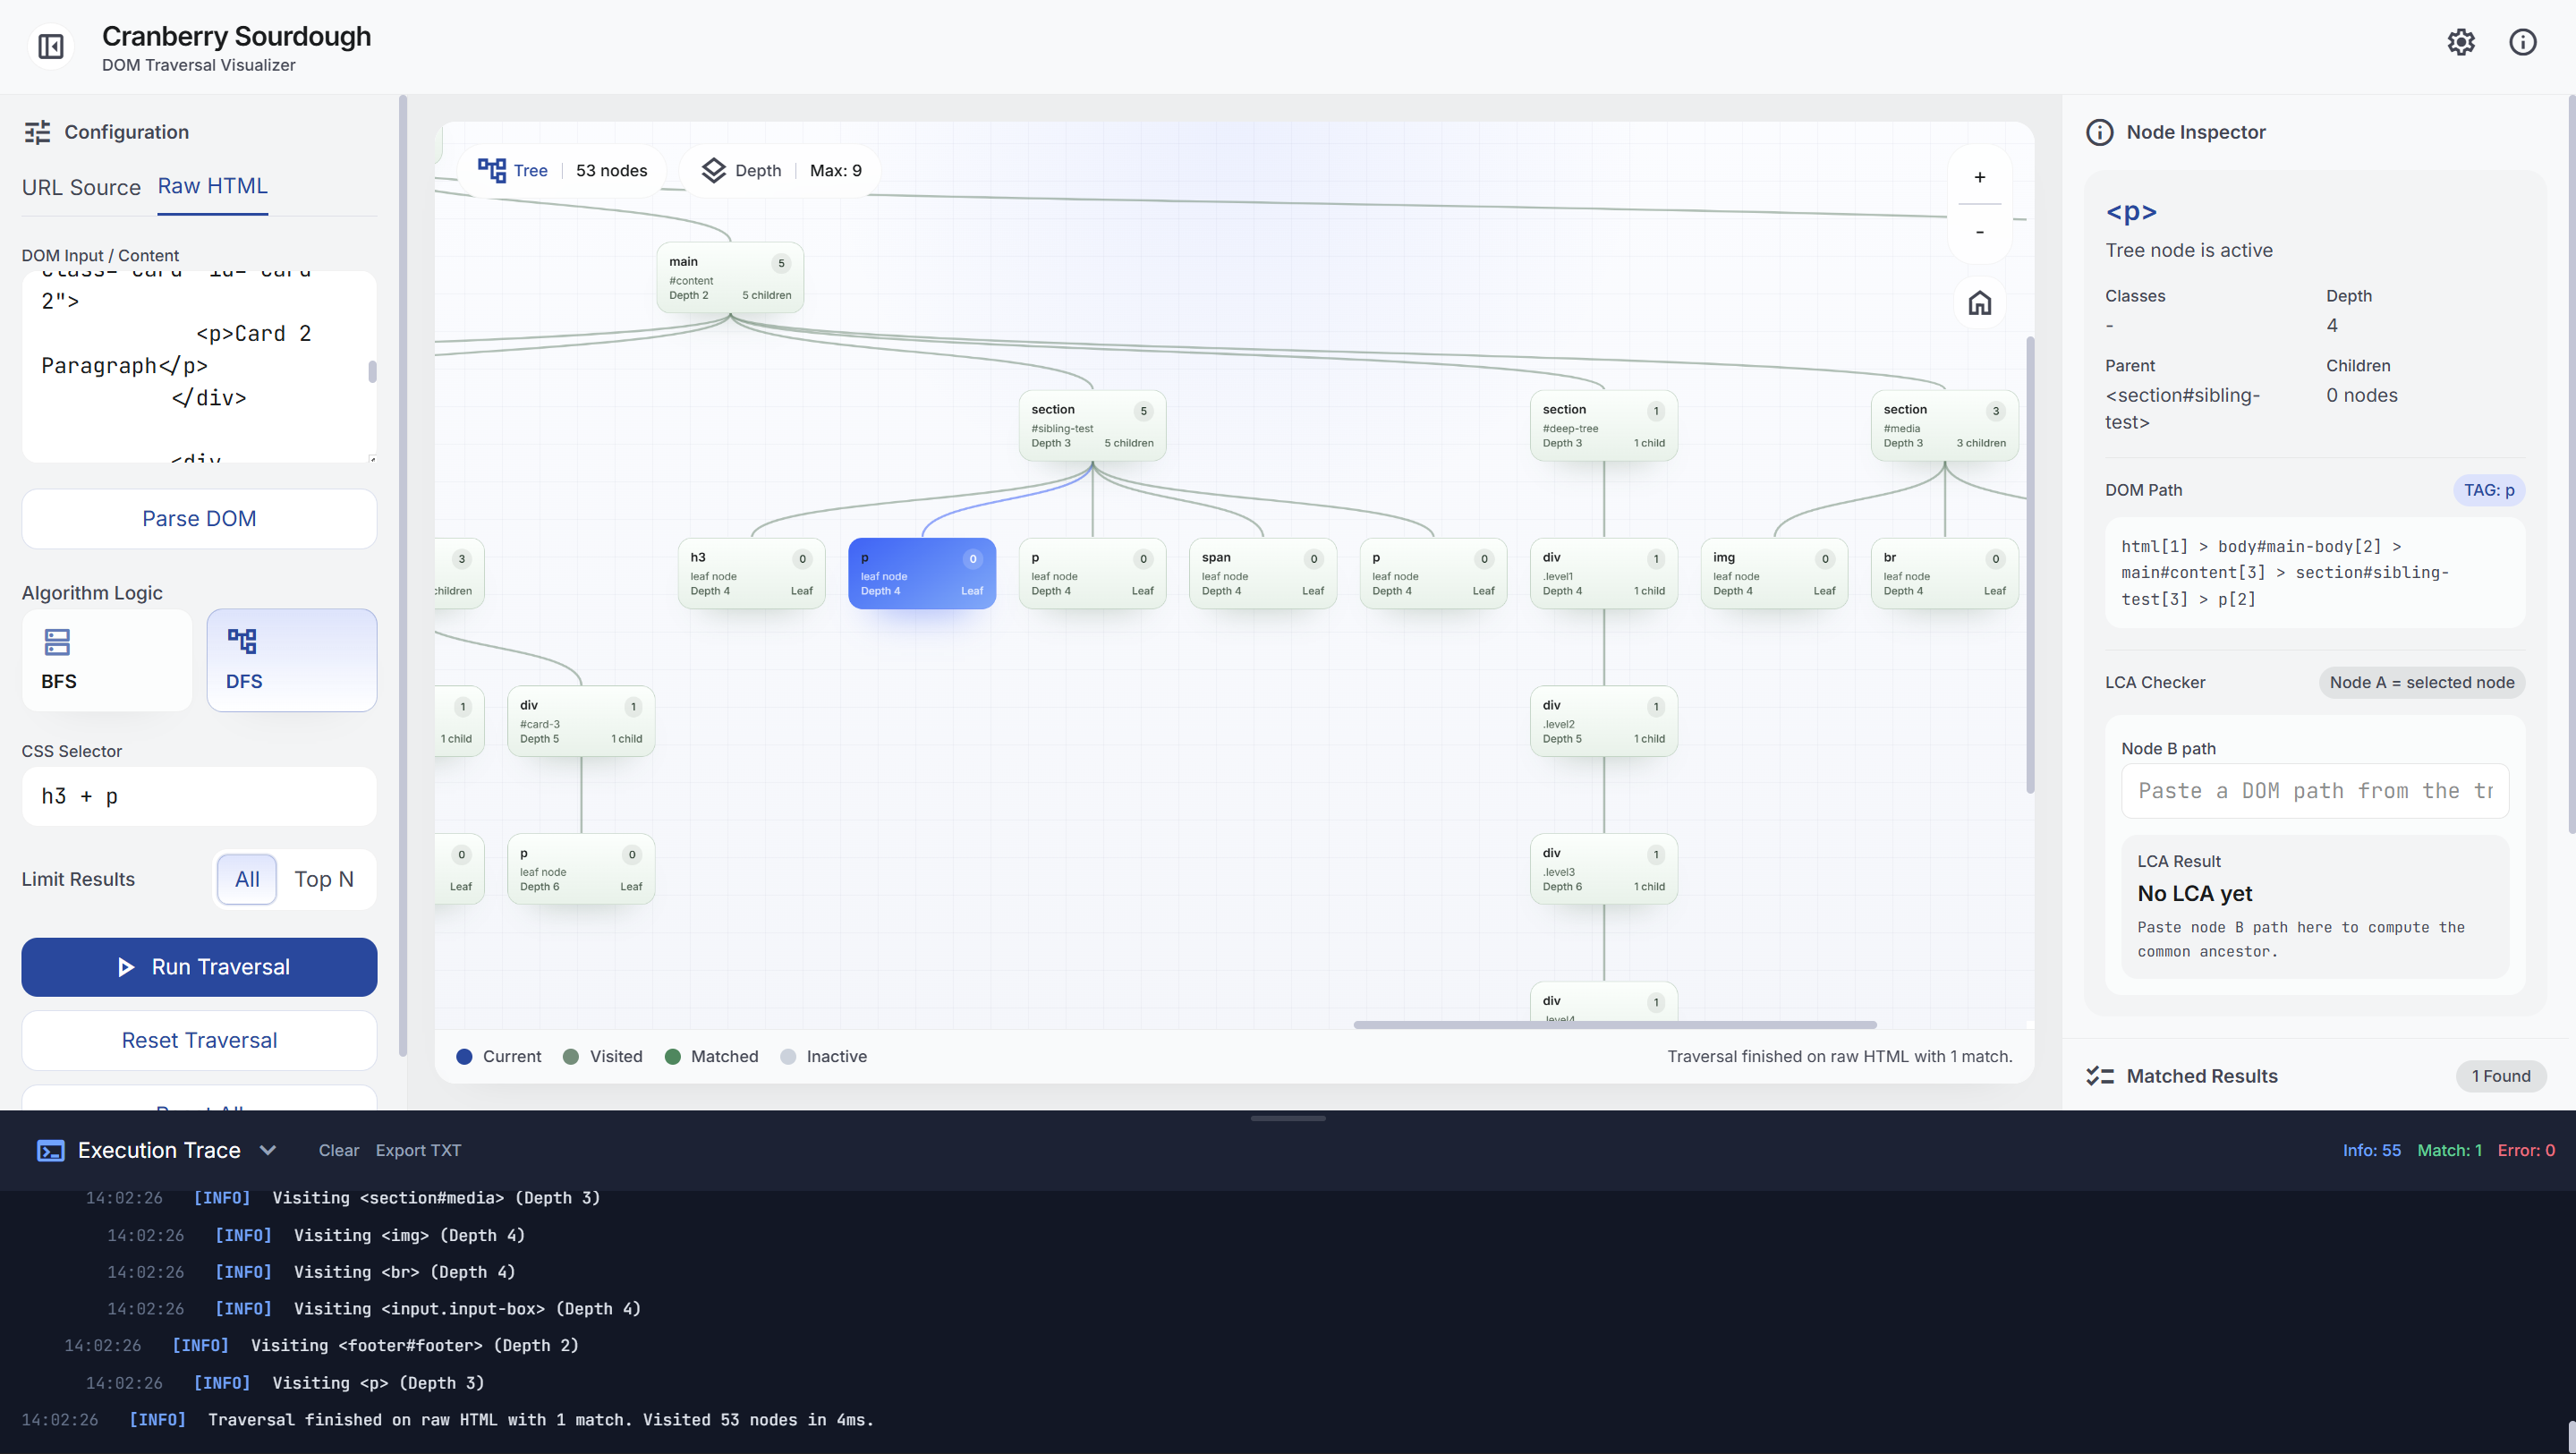
\includegraphics[width=10.5cm]{testcases/08.png}} \\ \hline
\textbf{Expected} & \textbf{Actual} \\ \hline
Selector \texttt{h3 + p} menampilkan sibling tepat setelah elemen.
&
Elemen p pertama yang merupakan sibling setelah h3 terdeteksi. \\ \hline
\end{tabular}
\caption{Pengujian Adjacent Sibling}
\end{table}

\subsection{General Sibling}

\begin{table}[H]
\centering
\renewcommand{\arraystretch}{1.4}
\begin{tabular}{|m{5.4cm}|m{5.4cm}|}
\hline
\multicolumn{2}{|c|}{\textbf{Snippet}} \\ \hline
\multicolumn{2}{|c|}{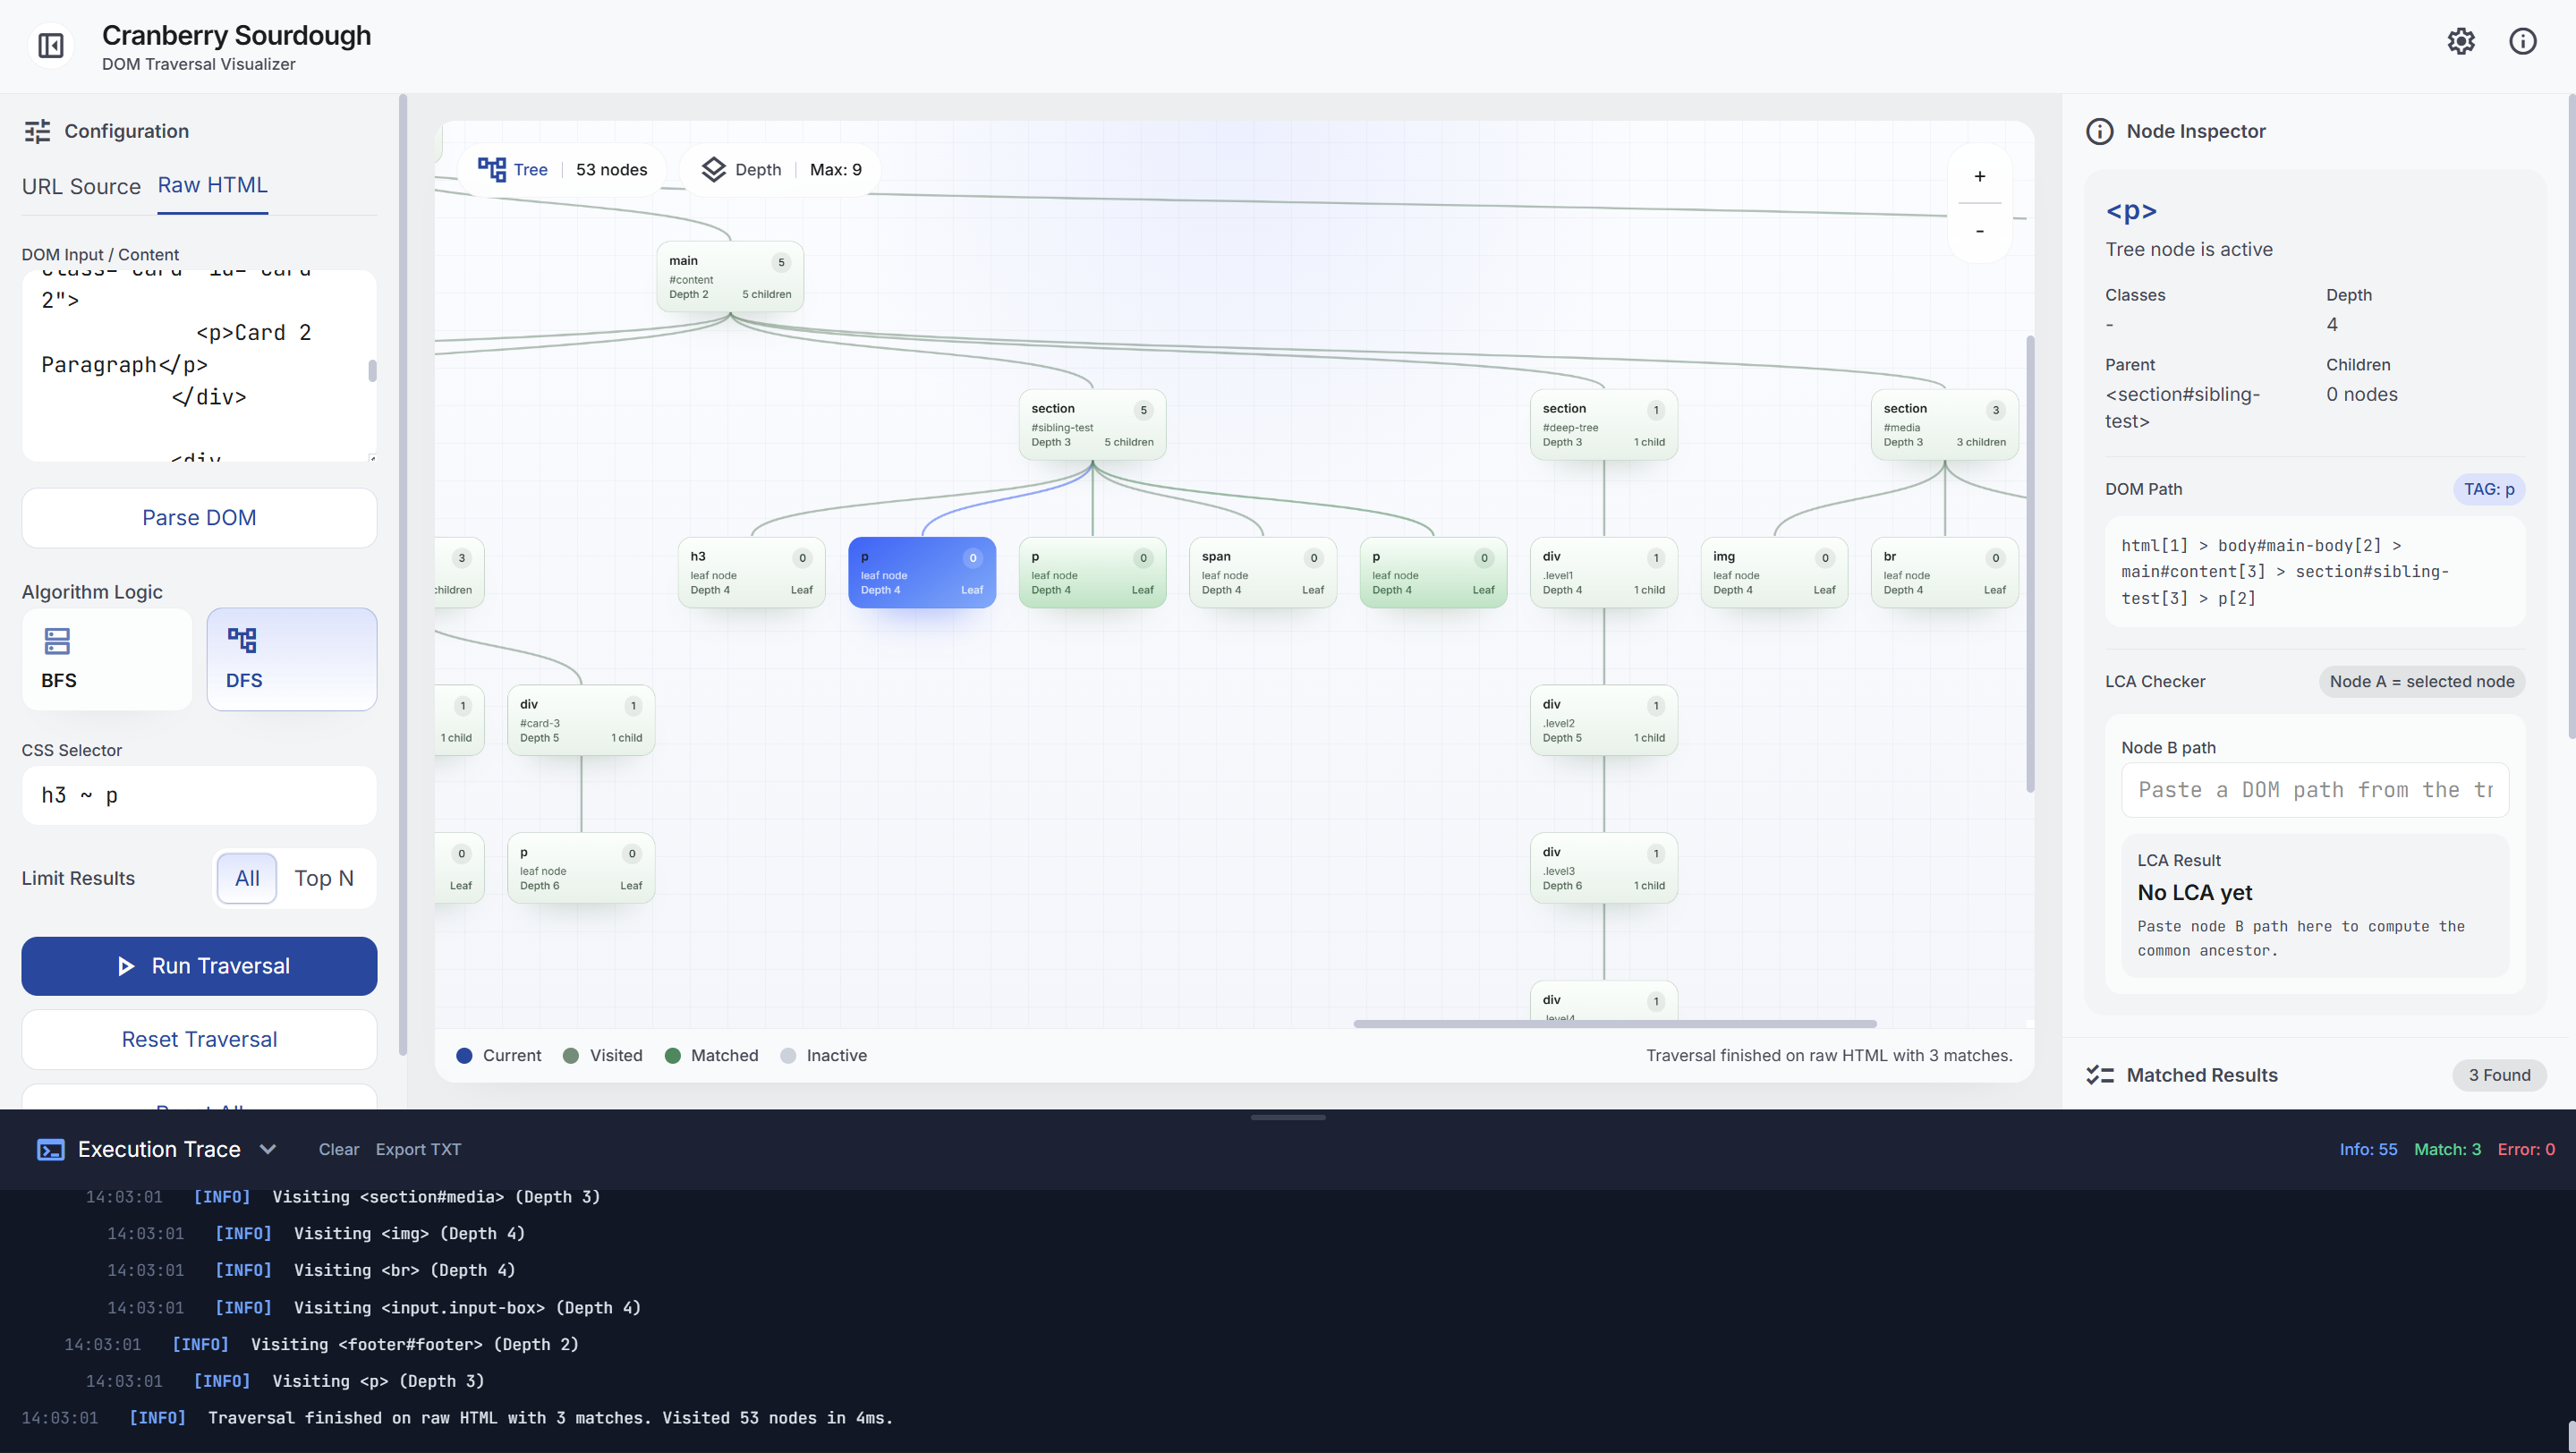
\includegraphics[width=10.5cm]{testcases/09.png}} \\ \hline
\textbf{Expected} & \textbf{Actual} \\ \hline
Selector \texttt{h3 ~ p} menampilkan seluruh sibling setelah elemen.
&
Elemen p yang merupakan sibling h3 terdeteksi.  \\ \hline
\end{tabular}
\caption{Pengujian General Sibling}
\end{table}

\subsection{BFS \& DFS}

\begin{table}[H]
\centering
\renewcommand{\arraystretch}{1.4}
\begin{tabular}{|m{5.4cm}|m{5.4cm}|}
\hline
\multicolumn{2}{|c|}{\textbf{Snippet}} \\ \hline
\multicolumn{2}{|c|}{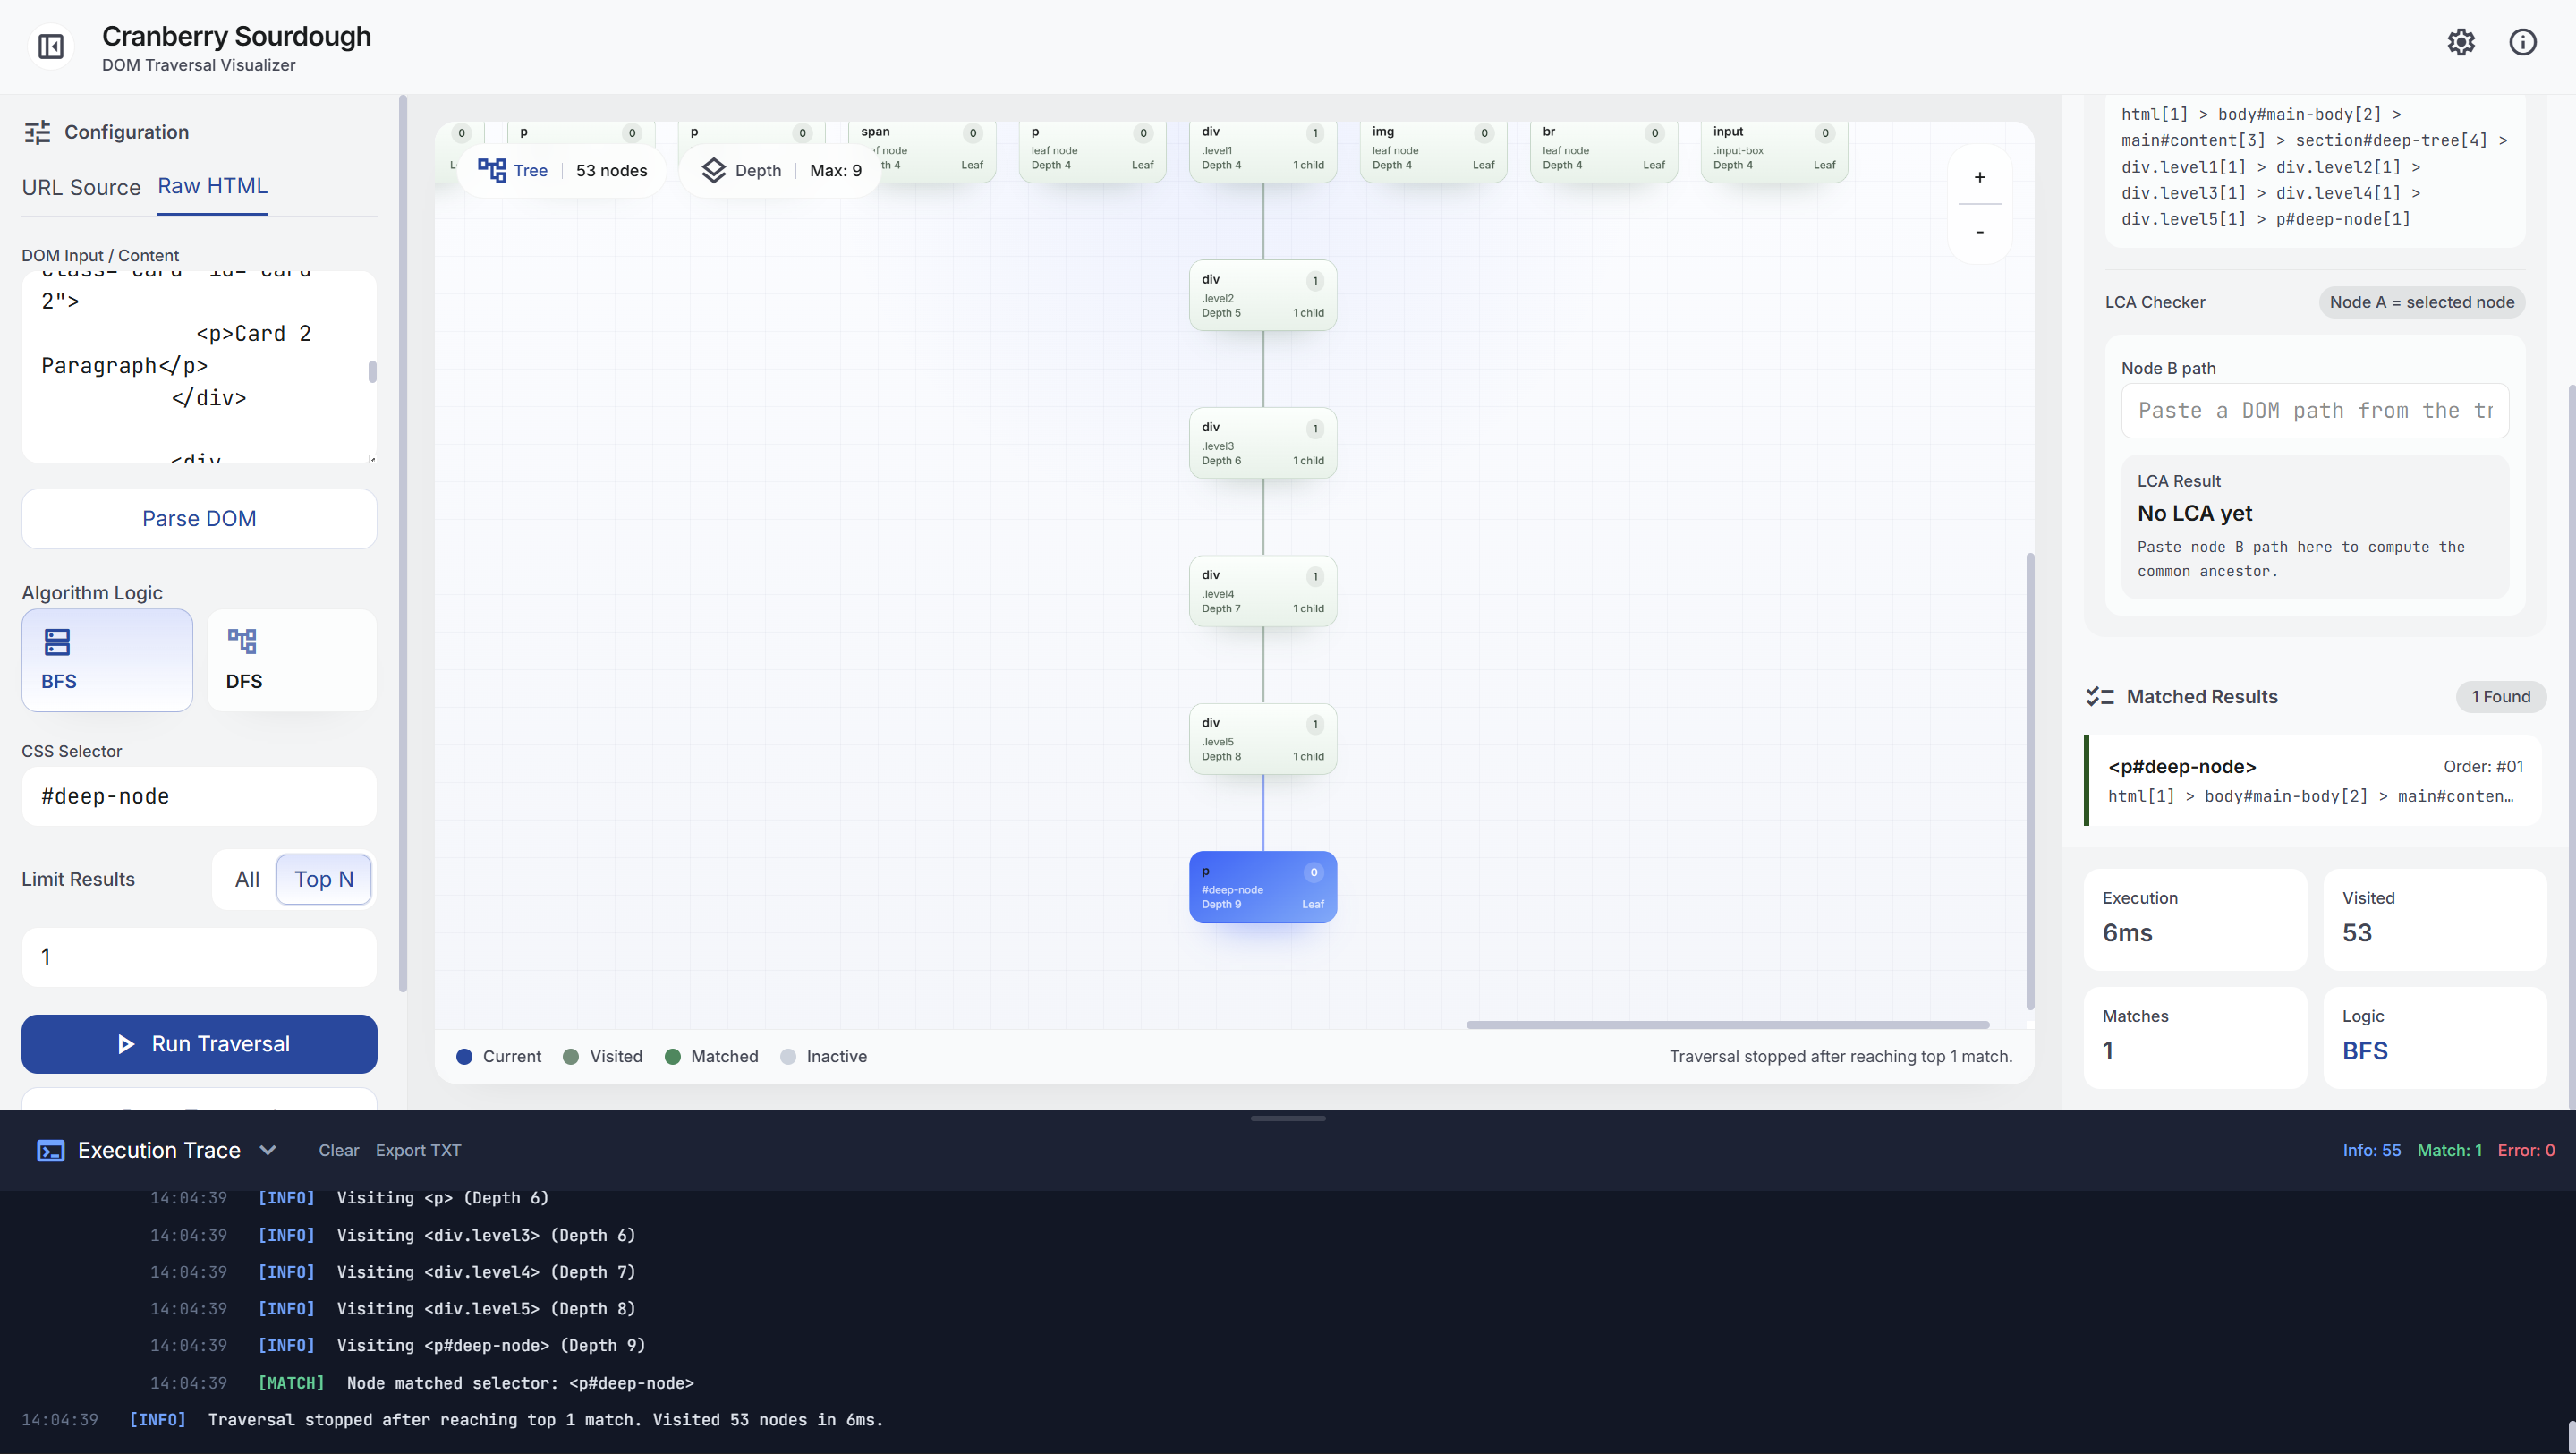
\includegraphics[width=10.5cm]{testcases/10-1.png}} \\ \hline
\textbf{Expected} & \textbf{Actual} \\ \hline
Traversal BFS berhasil menemukan node target.
&
BFS berhasil menemukan \#deep-node setelah mengunjungi 53 node. \\ \hline
\multicolumn{2}{|c|}{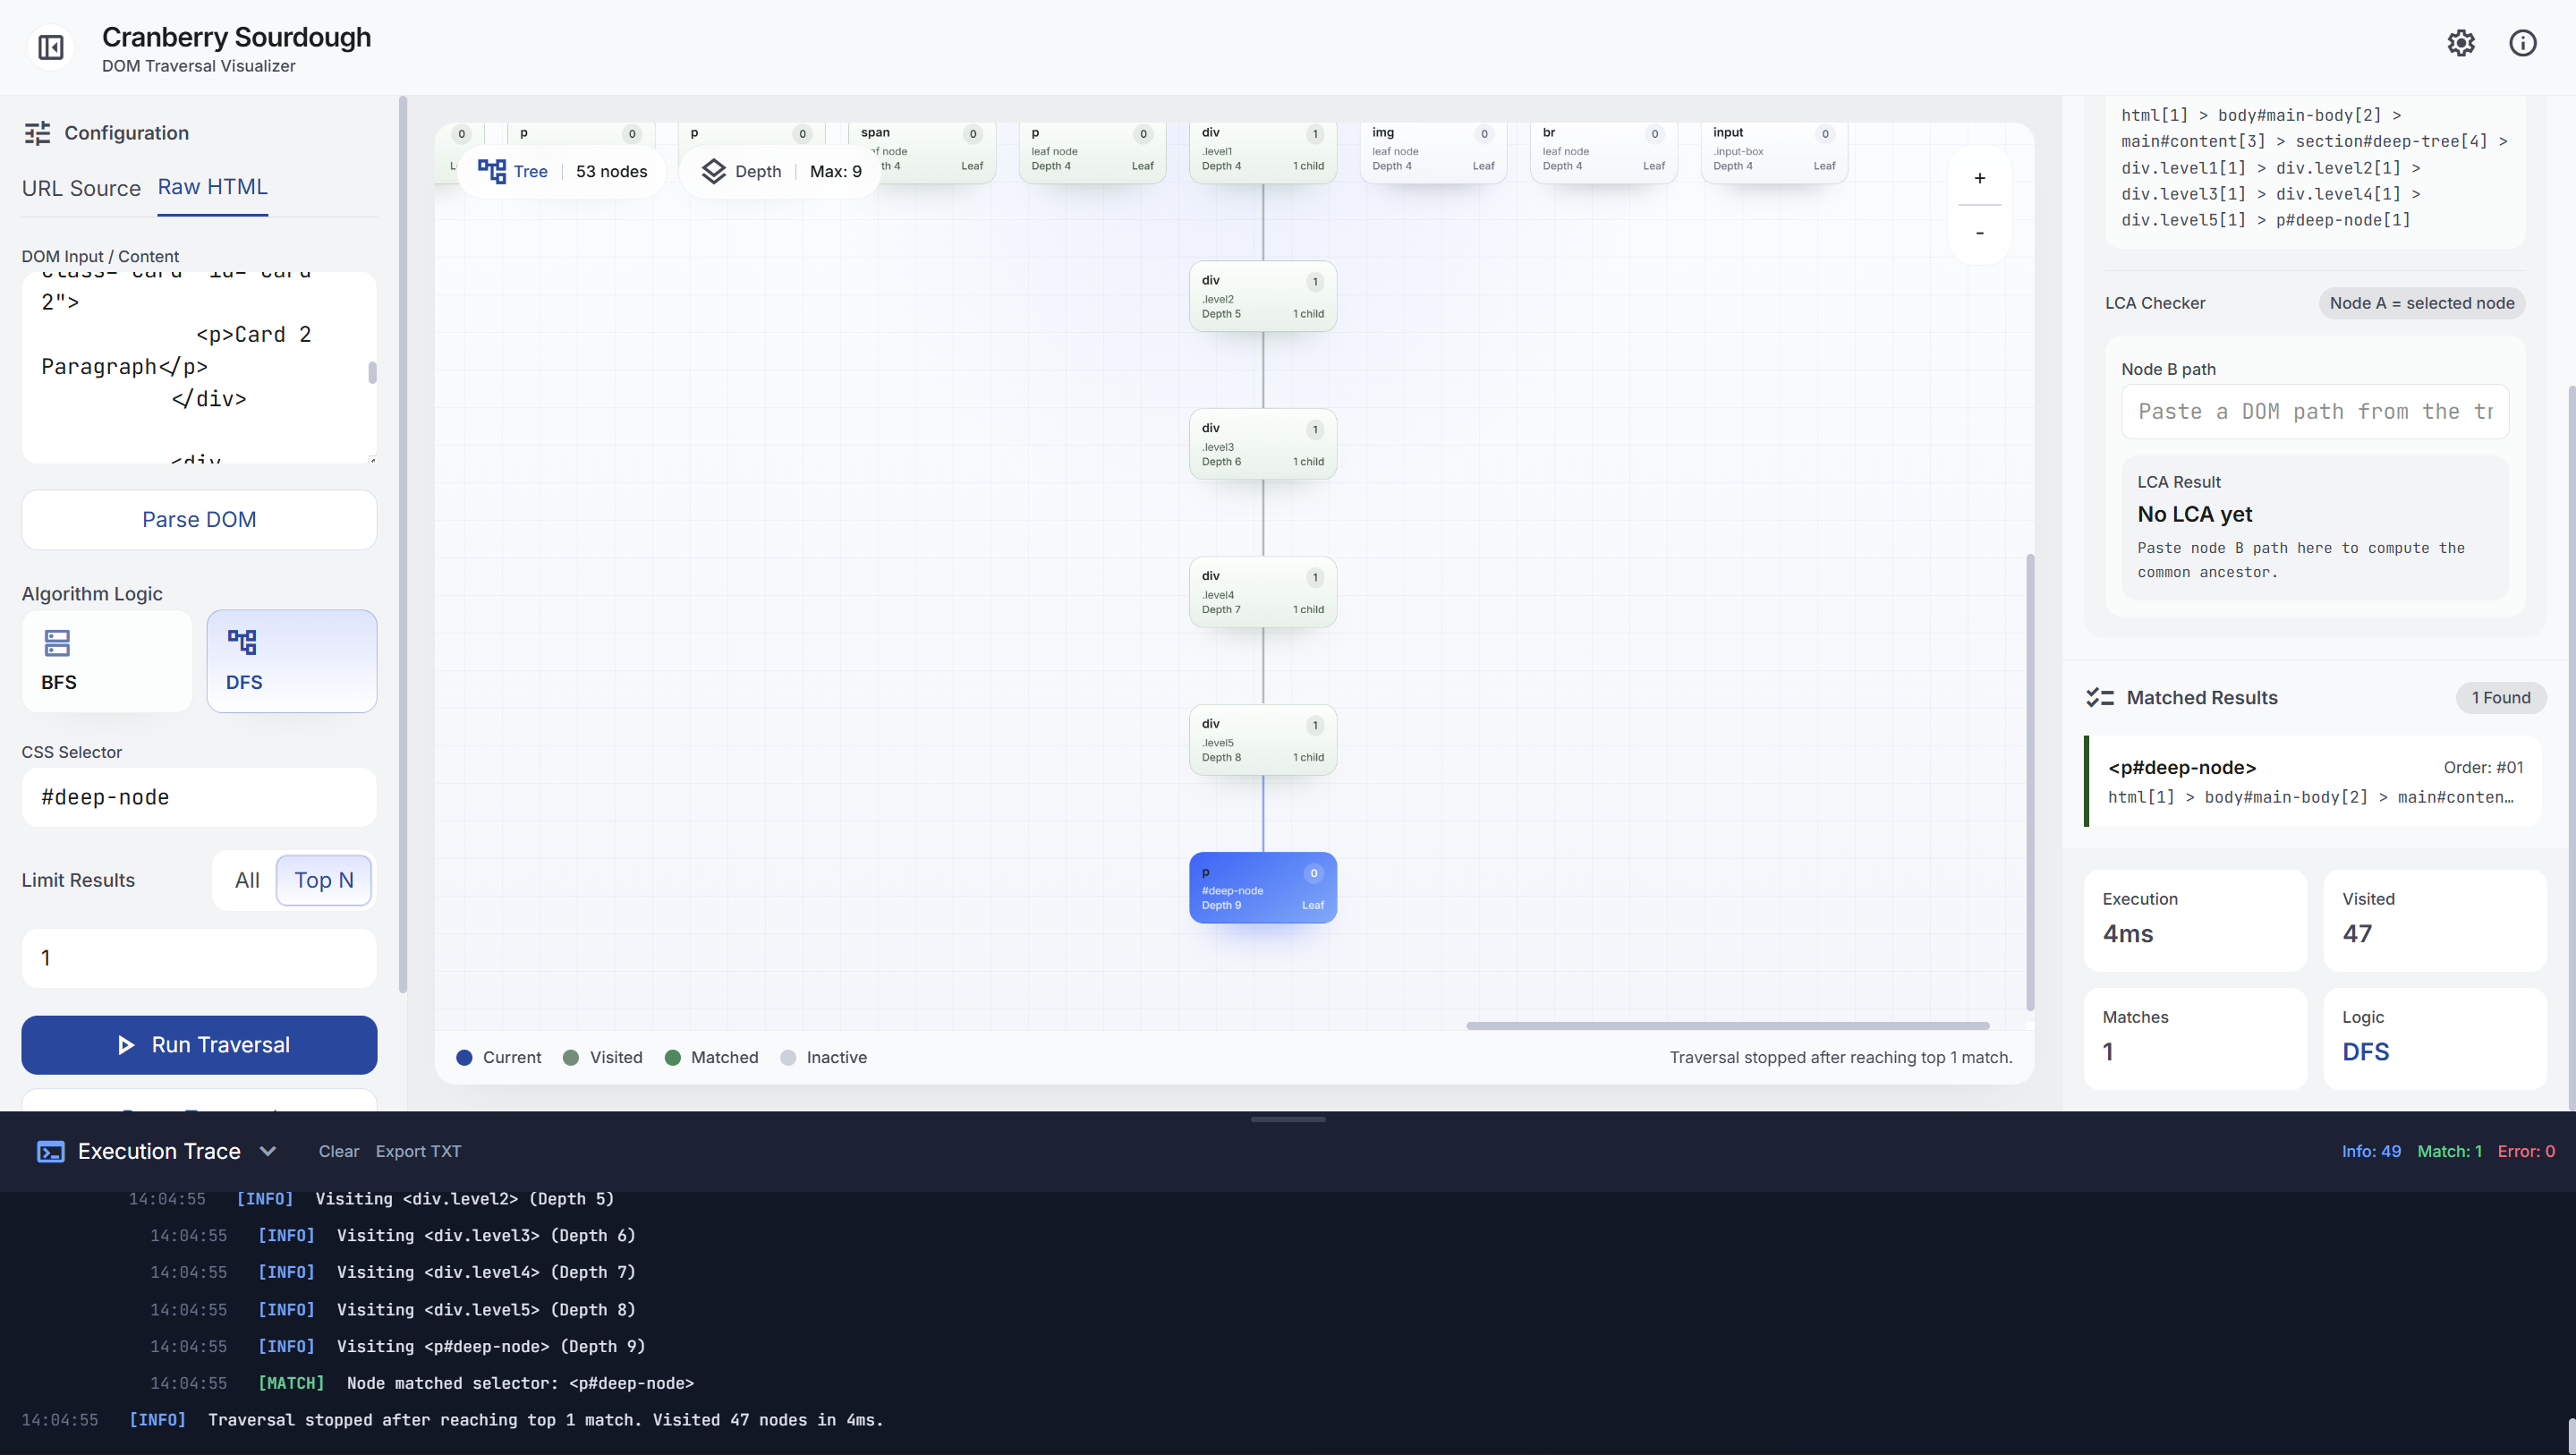
\includegraphics[width=10.5cm]{testcases/10-2.png}} \\ \hline
\textbf{Expected} & \textbf{Actual} \\ \hline
Traversal DFS berhasil menemukan node target.
&
DFS berhasil menemukan \#deep-node setelah mengunjungi 47 node. \\ \hline
\end{tabular}
\caption{Pengujian BFS dan DFS}
\end{table}

\subsection{Top N \& All}

\begin{table}[H]
\centering
\renewcommand{\arraystretch}{1.4}
\begin{tabular}{|m{5.4cm}|m{5.4cm}|}
\hline
\multicolumn{2}{|c|}{\textbf{Snippet}} \\ \hline
\multicolumn{2}{|c|}{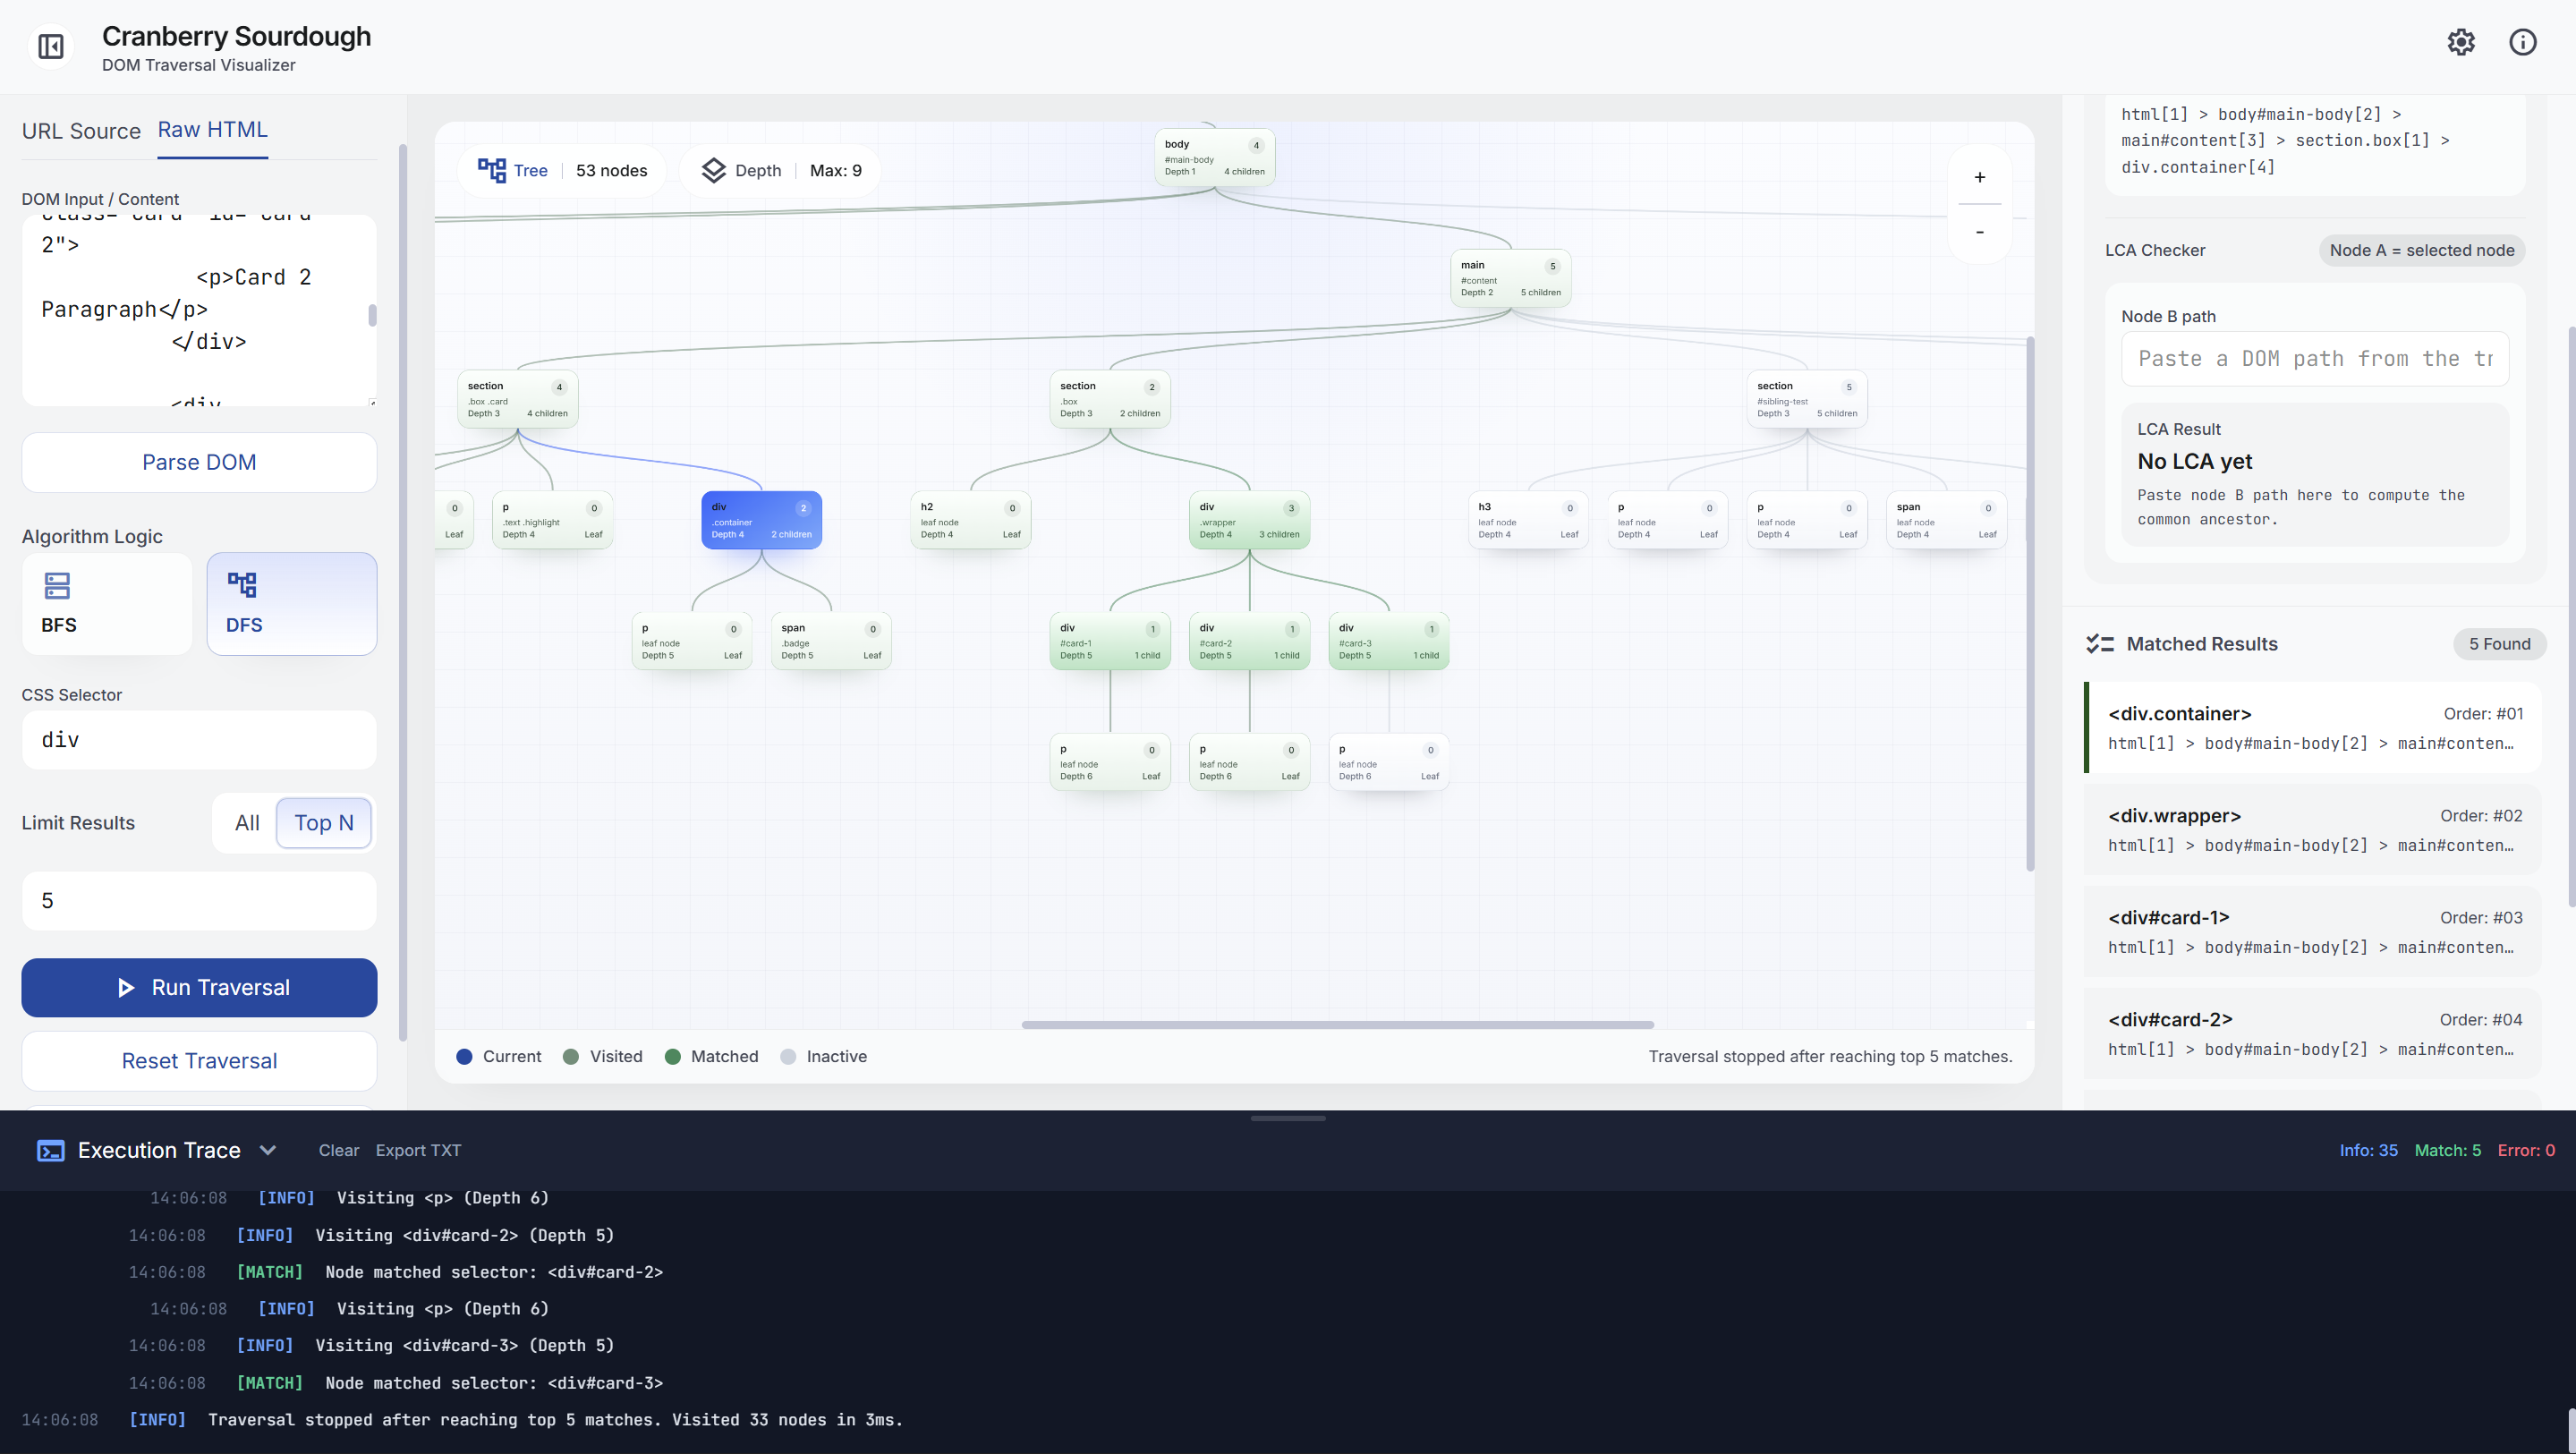
\includegraphics[width=10.5cm]{testcases/11-2.png}} \\ \hline
\textbf{Expected} & \textbf{Actual} \\ \hline
Fitur Top N menampilkan sejumlah hasil sesuai nilai N yang dimasukkan.
&
Top N berhasil menampilkan 5 elemen div yang ditemukan terlebih dahulu. \\ \hline
\multicolumn{2}{|c|}{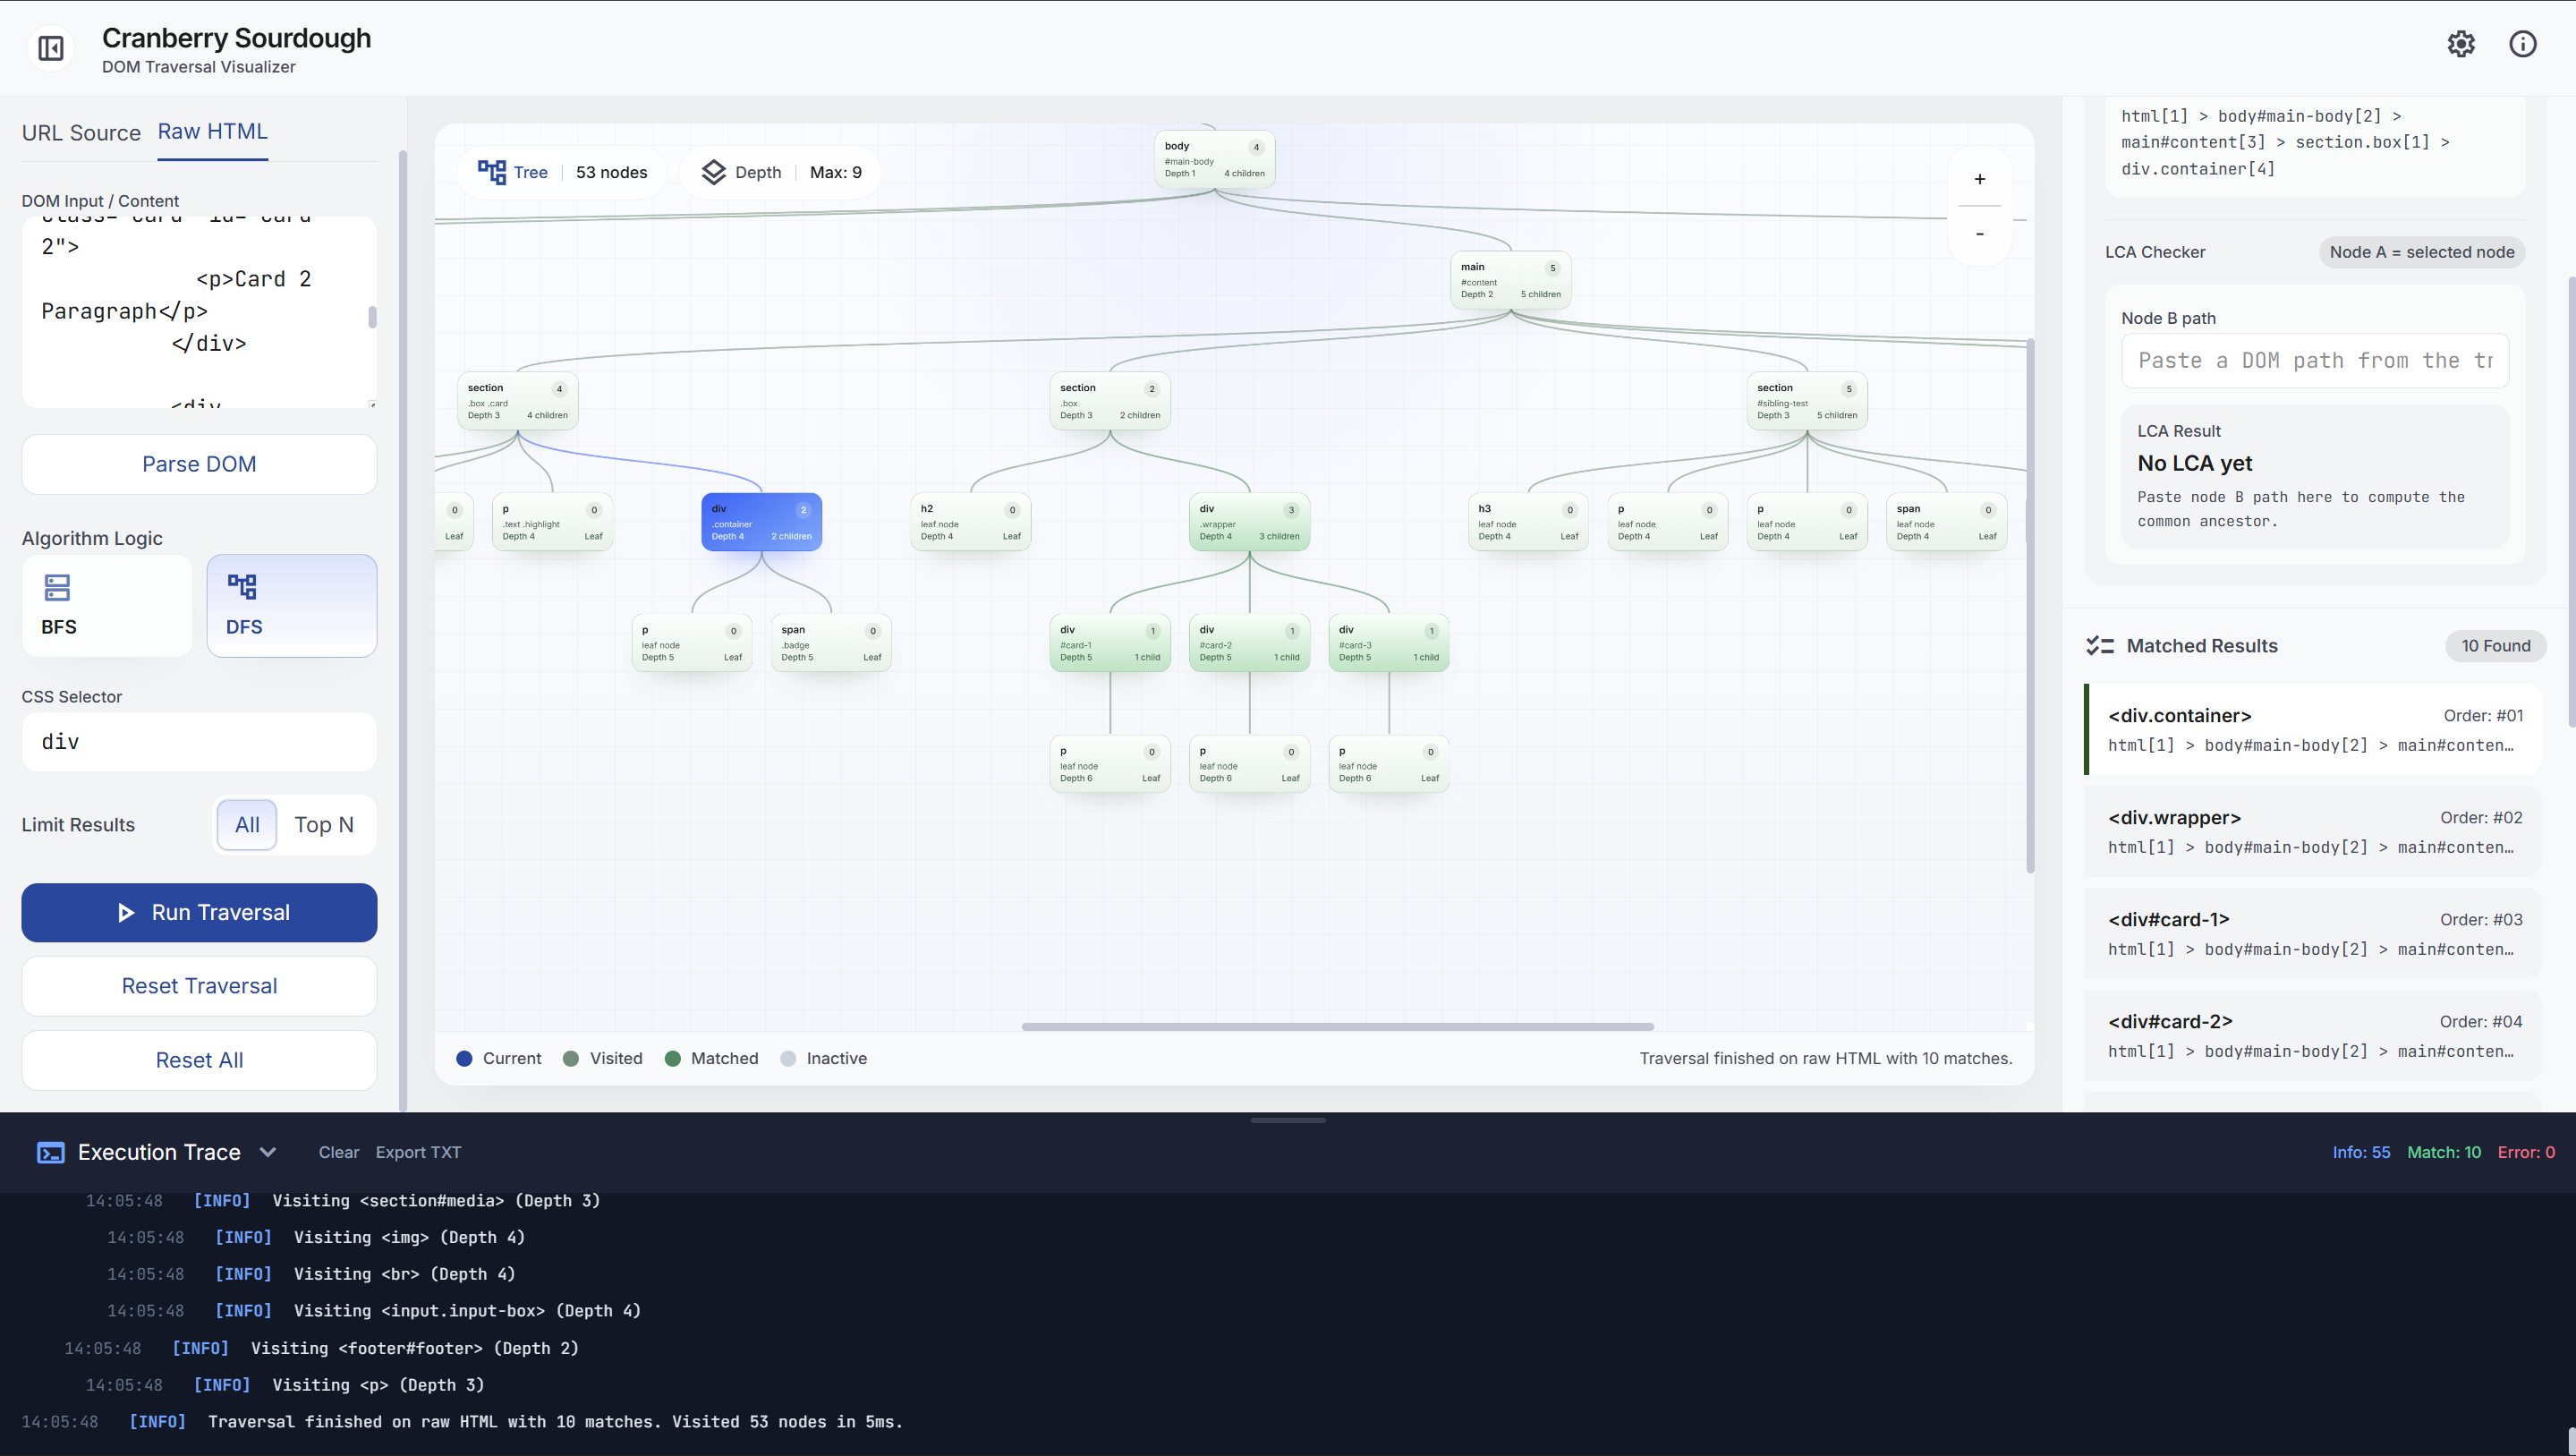
\includegraphics[width=10.5cm]{testcases/11-1.png}} \\ \hline
\textbf{Expected} & \textbf{Actual} \\ \hline
Fitur All menampilkan seluruh hasil pencarian tanpa batasan jumlah.
&
Fitur All berhasil menampilkan seluruh elemen div yang ditemukan. \\ \hline
\end{tabular}
\caption{Pengujian Top N dan All}
\end{table}

\subsection{Invalid Selector}

\begin{table}[H]
\centering
\renewcommand{\arraystretch}{1.4}
\begin{tabular}{|m{5.4cm}|m{5.4cm}|}
\hline
\multicolumn{2}{|c|}{\textbf{Snippet}} \\ \hline
\multicolumn{2}{|c|}{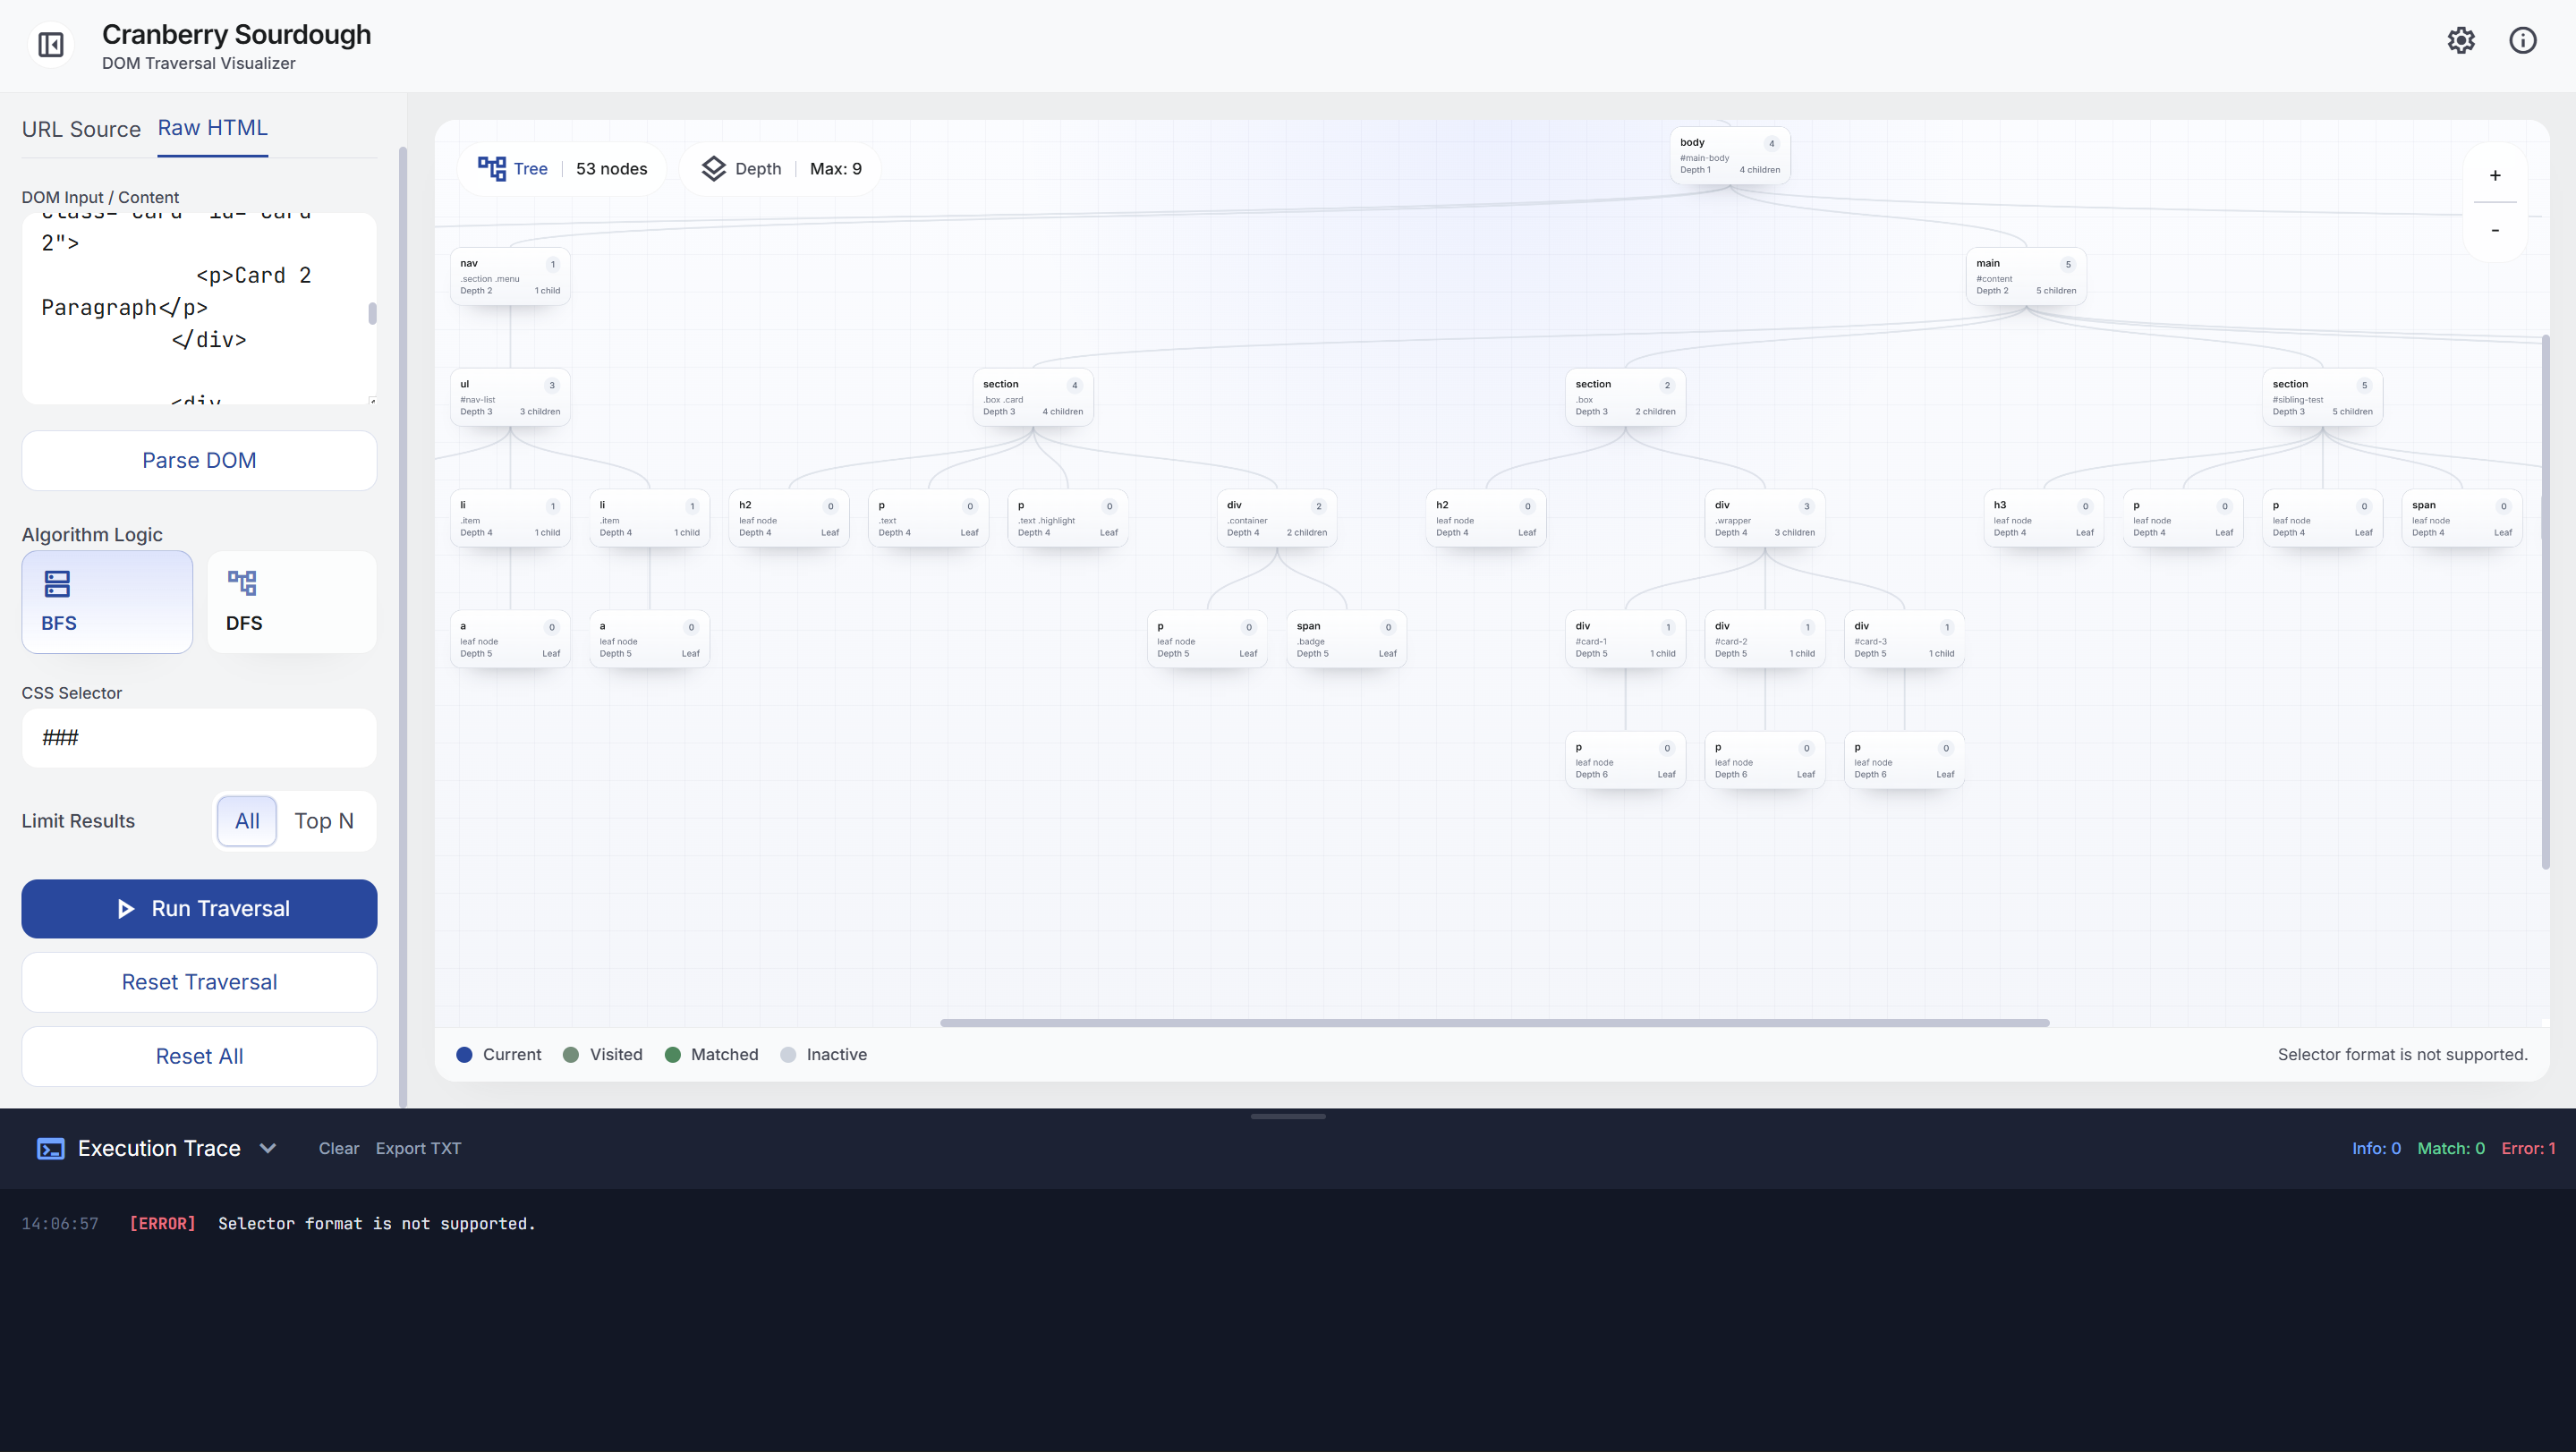
\includegraphics[width=10.5cm]{testcases/12.png}} \\ \hline
\textbf{Expected} & \textbf{Actual} \\ \hline
Selector tidak valid menghasilkan pesan error.
&
Execution trace berhasil memberikan \textit{graceful error handling} akibat format selector yang tidak sesuai. \\ \hline
\end{tabular}
\caption{Pengujian Invalid Selector}
\end{table}

\subsection{Nonexistent Selector}

\begin{table}[H]
\centering
\renewcommand{\arraystretch}{1.4}
\begin{tabular}{|m{5.4cm}|m{5.4cm}|}
\hline
\multicolumn{2}{|c|}{\textbf{Snippet}} \\ \hline
\multicolumn{2}{|c|}{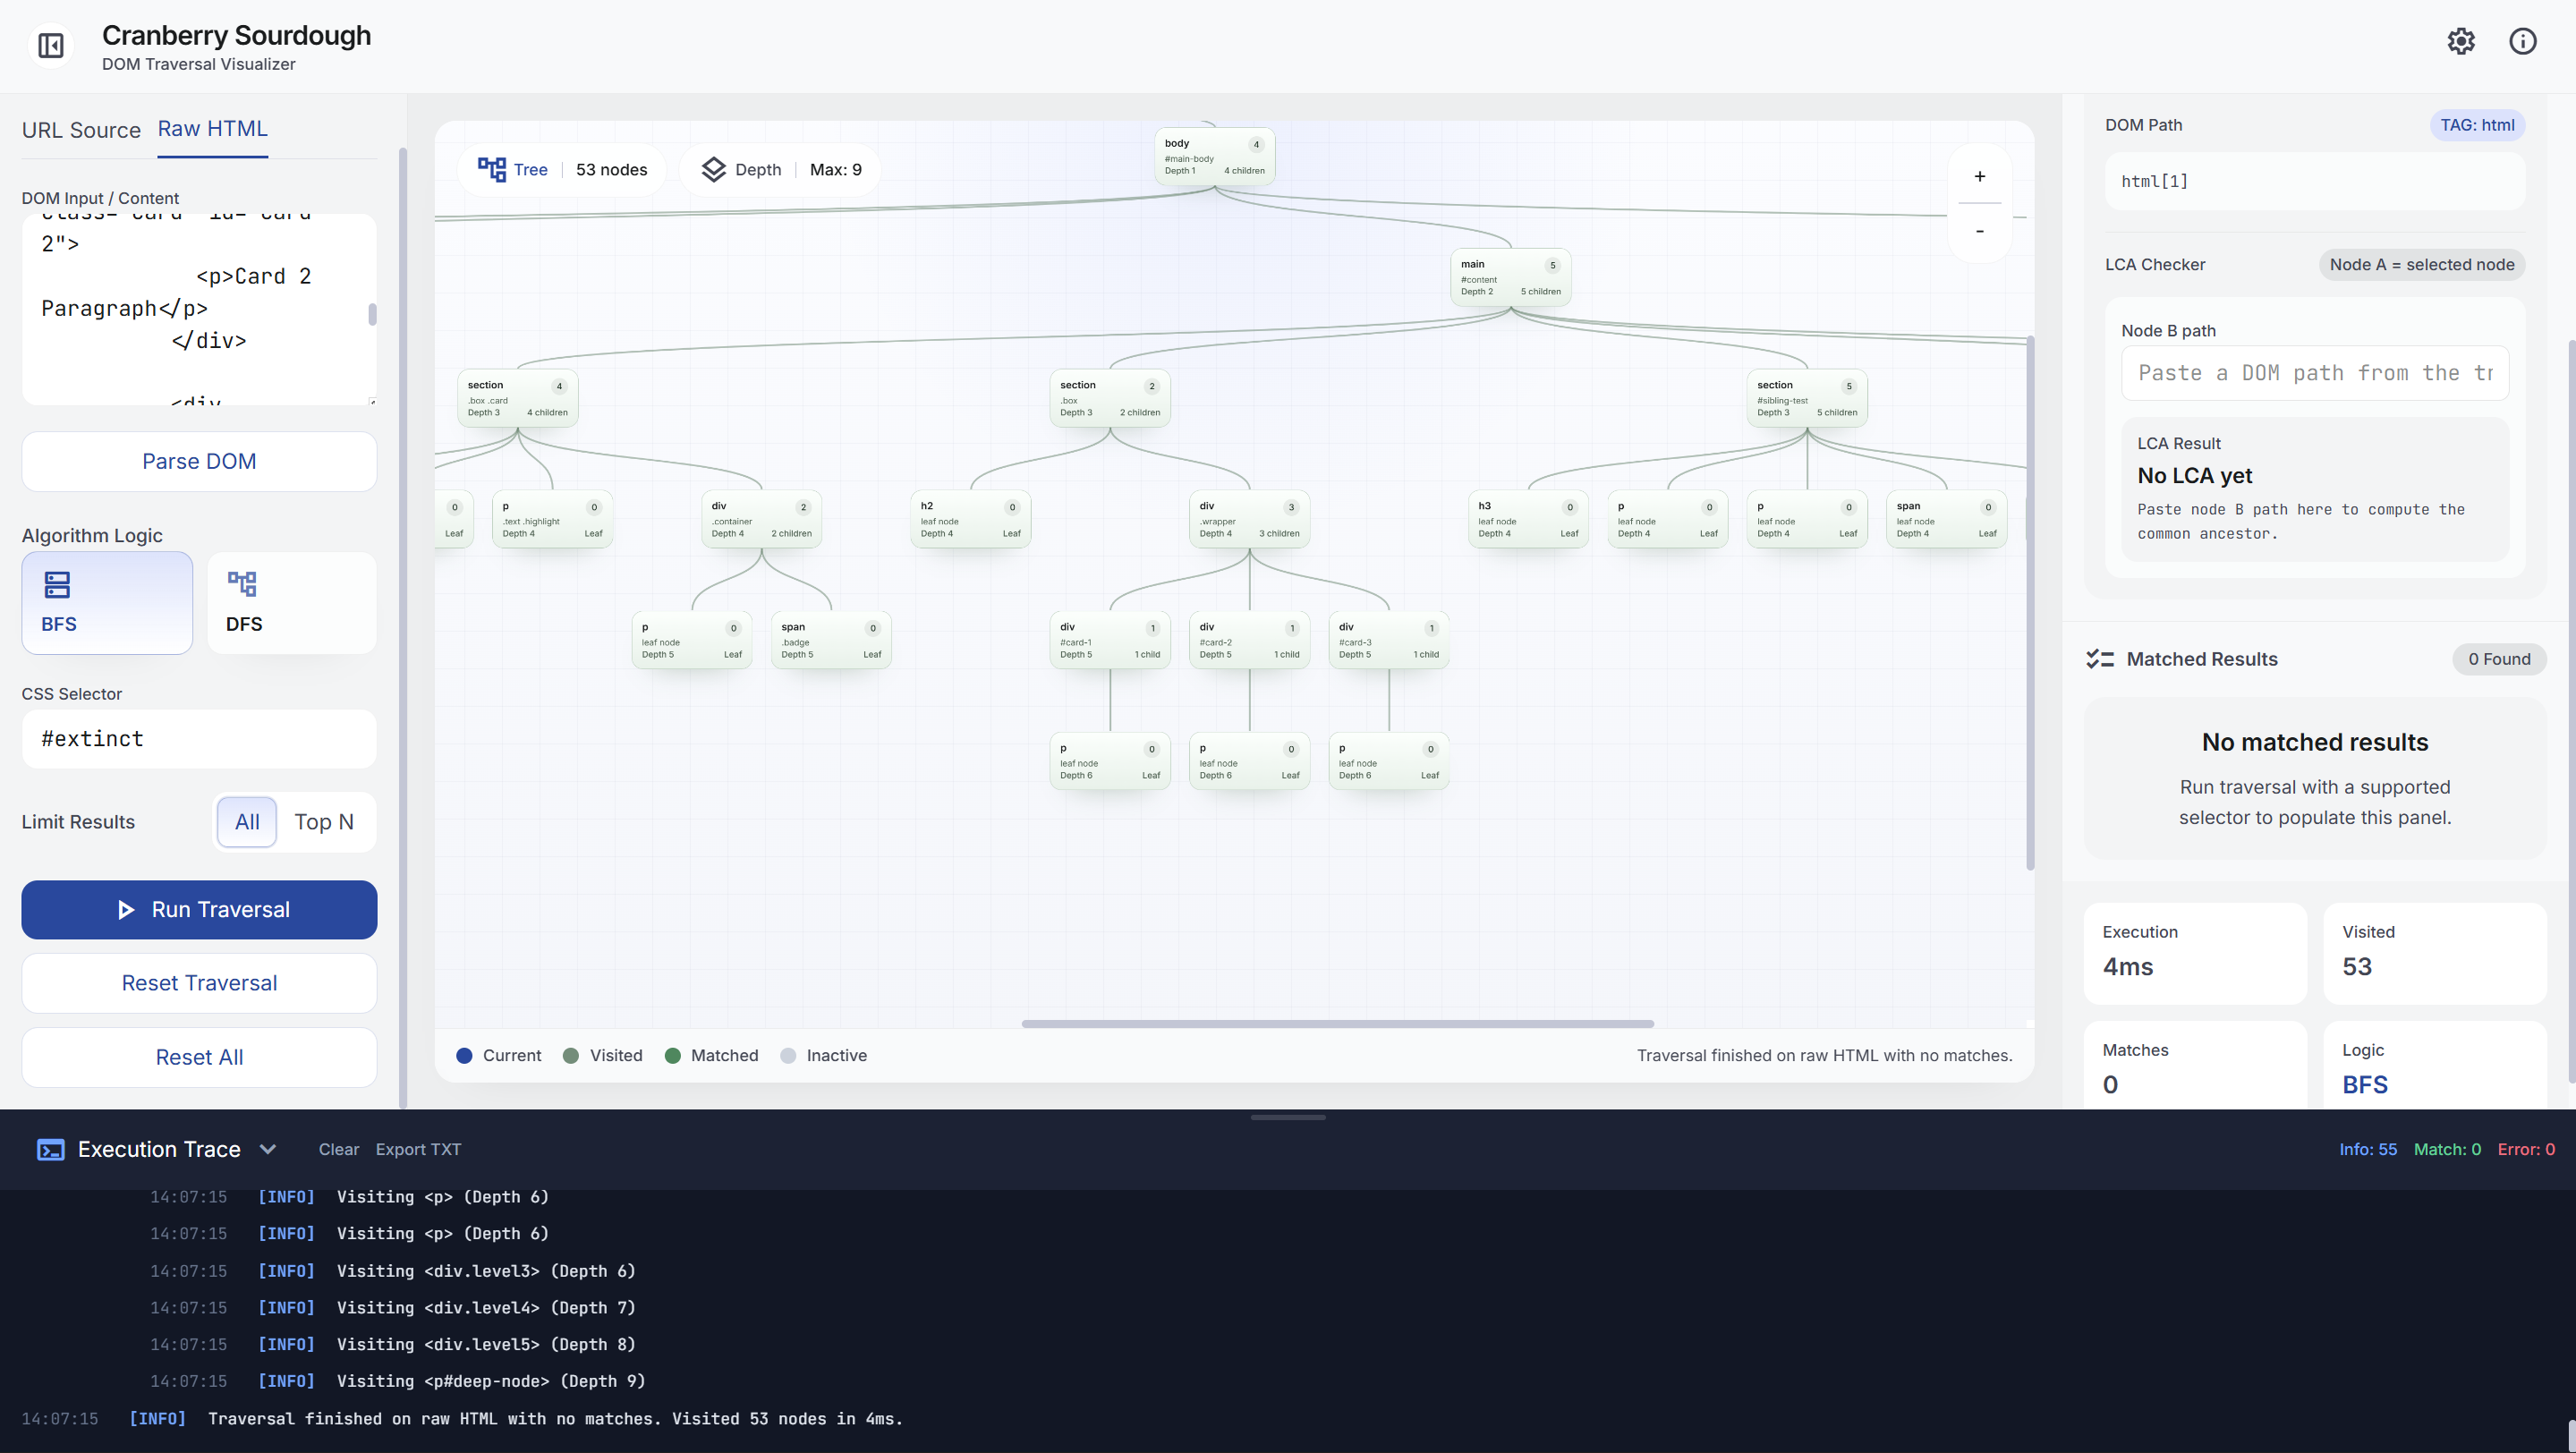
\includegraphics[width=10.5cm]{testcases/13.png}} \\ \hline
\textbf{Expected} & \textbf{Actual} \\ \hline
Selector valid tetapi tidak ditemukan menghasilkan 0 hasil.
&
Penelusuran berhasil dilakukan dengan hasil tidak ditemukan. \\ \hline
\end{tabular}
\caption{Pengujian Nonexistent Selector}
\end{table}

\subsection{Multithreading}

\begin{table}[H]
\centering
\renewcommand{\arraystretch}{1.4}
\begin{tabular}{|m{5.4cm}|m{5.4cm}|}
\hline
\multicolumn{2}{|c|}{\textbf{Snippet}} \\ \hline
\multicolumn{2}{|c|}{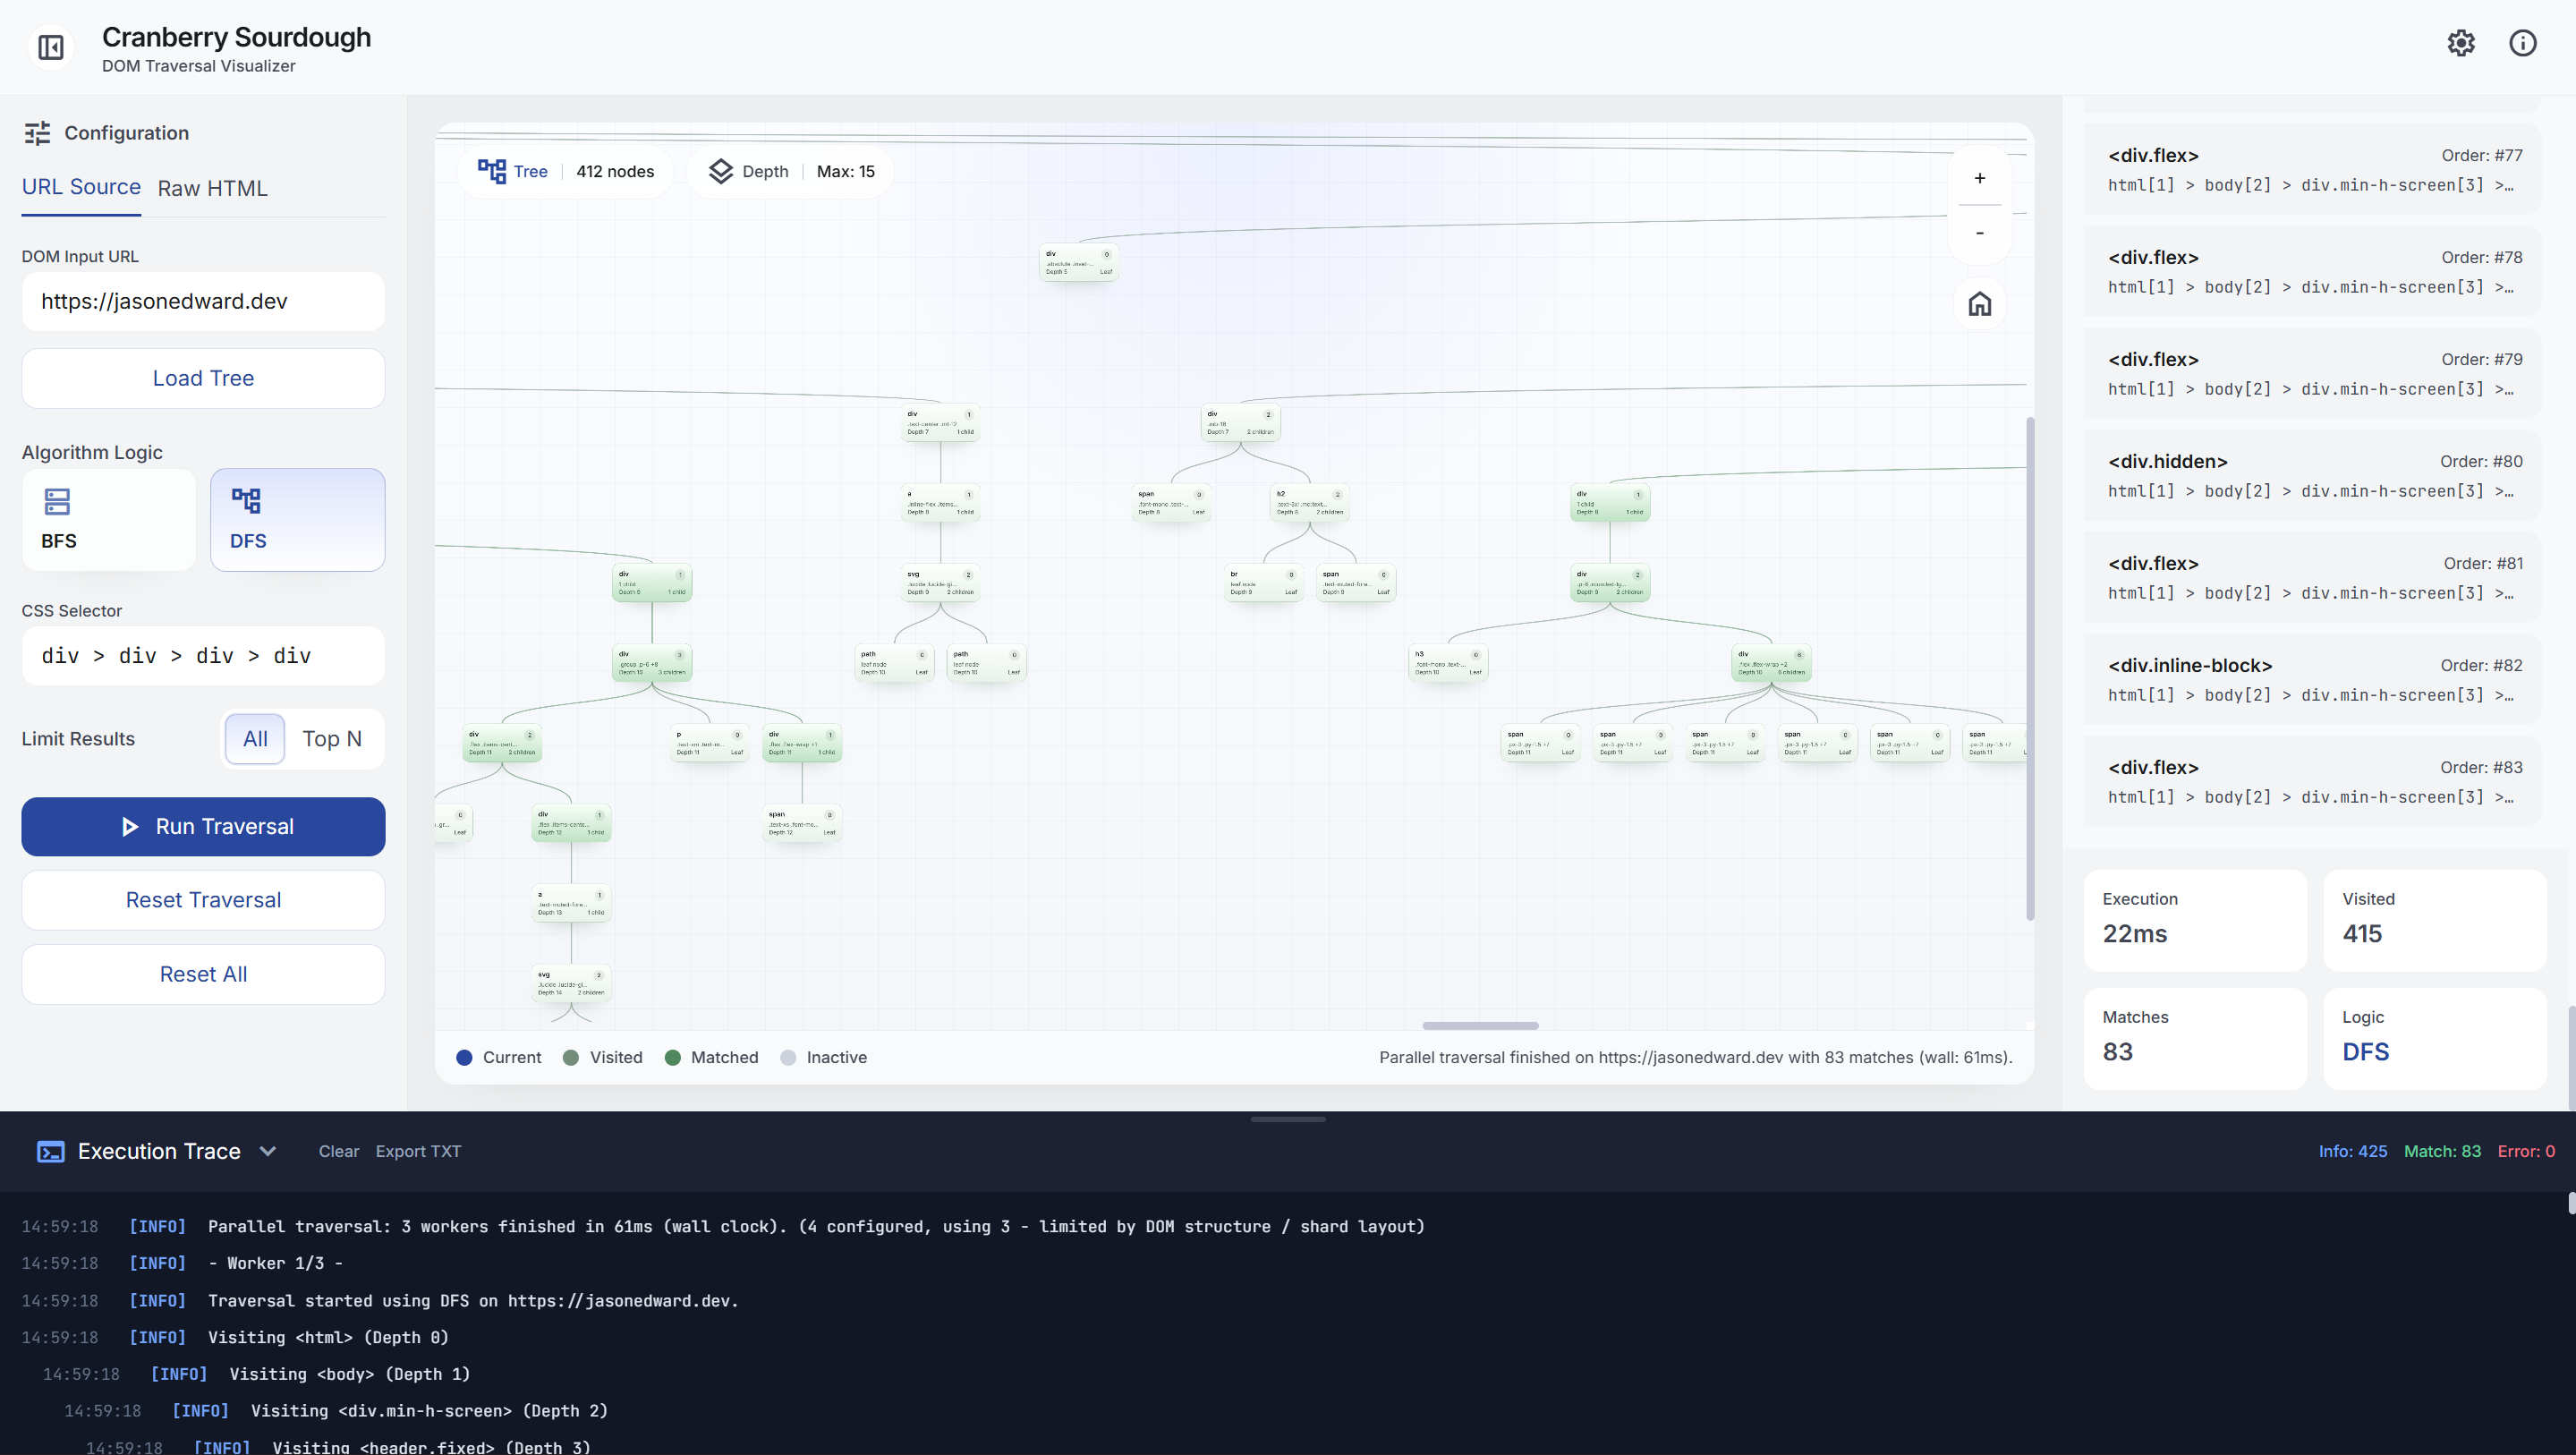
\includegraphics[width=10.5cm]{testcases/14.png}} \\ \hline
\textbf{Expected} & \textbf{Actual} \\ \hline
Fitur multithreading berjalan dengan benar dan proses traversal dapat dieksekusi secara paralel tanpa error.
&
Multithreading dapat dijalankan namun hanya memberikan tambahan kecepatan yang tidak begitu signifikan. \\ \hline
\end{tabular}
\caption{Pengujian Multithreading}
\end{table}

\subsection{LCA Binary Lifting}

\begin{table}[H]
\centering
\renewcommand{\arraystretch}{1.4}
\begin{tabular}{|m{5.4cm}|m{5.4cm}|}
\hline
\multicolumn{2}{|c|}{\textbf{Snippet}} \\ \hline
\multicolumn{2}{|c|}{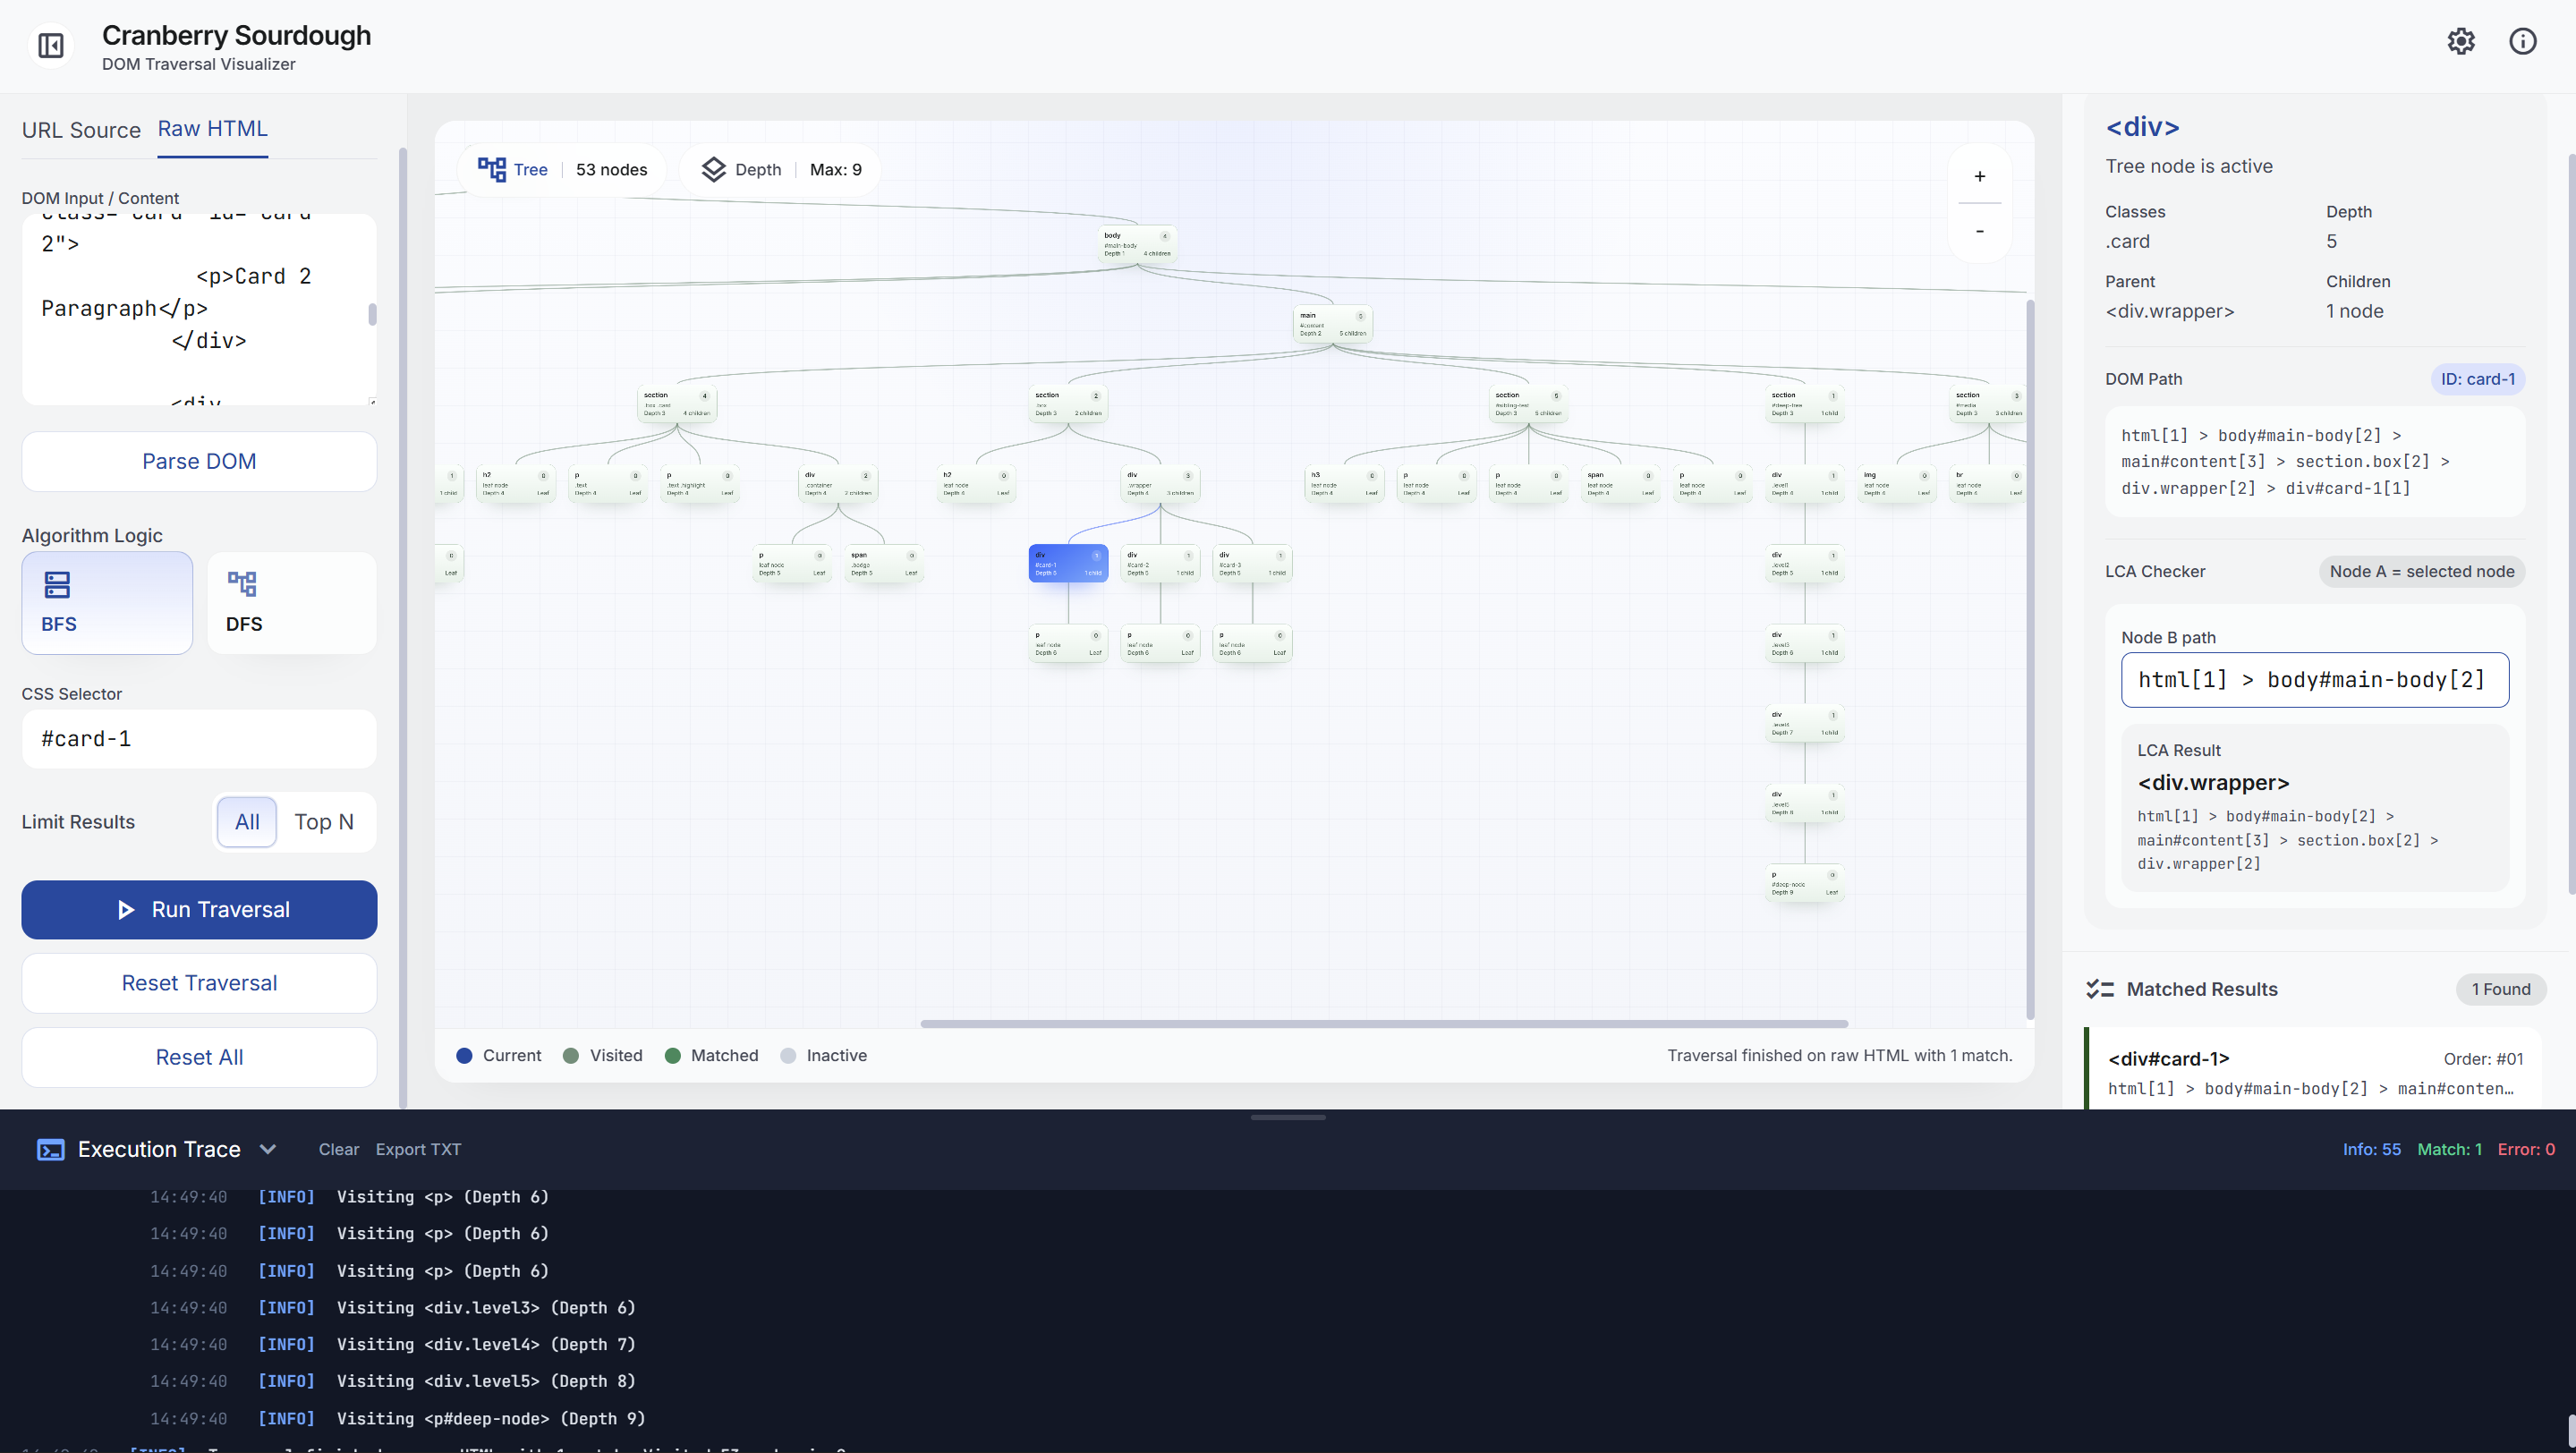
\includegraphics[width=10.5cm]{testcases/15.png}} \\ \hline
\textbf{Expected} & \textbf{Actual} \\ \hline
Fitur Lowest Common Ancestor dengan metode Binary Lifting menghasilkan ancestor bersama terdekat secara benar.
&
Ketika select \#card-1 dan \#card-2, maka sesuai struktur DOM didapatkan Lowest Common Ancestor keduanya adalah div.wrapper. \\ \hline
\end{tabular}
\caption{Pengujian LCA Binary Lifting}
\end{table}